% !Mode:: "TeX:UTF-8"

\def \xuewei{Master} % 定义学位 Doctor or Master

\def\xueke{Engineering} % 定义学科 Engineering, Science, Management, or Arts

\documentclass[12pt,openany,oneside]{book} 

\input{setup/type.tex}    % 硕博类型
\input{setup/package.tex} % 引用的宏包
\graphicspath{{figures/}} %定义所有的eps文件在 figures 子目录下

\begin{document}

% !Mode:: "TeX:UTF-8" 

%避免宏包 hyperref 和 arydshln 不兼容带来的目录链接失效的问题。
%\def\temp{\relax}
%\let\temp\addcontentsline
%\gdef\addcontentsline{\phantomsection\temp}

\makeatletter
\gdef\hitempty{}

%重新定义BiChapter命令,可实现标题手动换行,但不影响目录
%\def\BiChapter{\relax\@ifnextchar [{\@BiChapter}{\@@BiChapter}}
%\def\@BiChapter[#1]#2#3{\chapter[#1]{#2}
%    \addcontentsline{toe}{chapter}{\bfseries \xiaosi Chapter \thechapter \hspace{0.5em} #3}}
%\def\@@BiChapter#1#2{\chapter{#1}
%    \addcontentsline{toe}{chapter}{\bfseries \xiaosi Chapter \thechapter \hspace{0.5em}{\boldmath #2}}}
%
%\newcommand{\BiSection}[2]
%{   \section{#1}
%    \addcontentsline{toe}{section}{\protect\numberline{\csname thesection\endcsname}#2}
%}

%\newcommand{\BiSubsection}[2]
%{    \subsection{#1}
%    \addcontentsline{toe}{subsection}{\protect\numberline{\csname thesubsection\endcsname}#2}
%}

%\newcommand{\BiSubsubsection}[2]
%{    \subsubsection{#1}
%    \addcontentsline{toe}{subsubsection}{\protect\numberline{\csname thesubsubsection\endcsname}#2}
%}

%\newcommand{\BiAppendixChapter}[2] % 该附录命令适用于发表文章,简历等
%{\phantomsection
%\markboth{#1}{#1}
%\addcontentsline{toc}{chapter}{\xiaosi #1}
%\addcontentsline{toe}{chapter}{\bfseries \xiaosi #2}  \chapter*{#1}
%}

%\newcommand{\BiAppChapter}[2]    % 该附录命令适用于有章节的完整附录
%{\phantomsection 
% \chapter{#1}
% \addcontentsline{toe}{chapter}{\bfseries \xiaosi Appendix \thechapter~~#2}
%}

%\renewcommand{\thefigure}{\arabic{chapter}-\arabic{figure}}%使图编号为 7-1 的格式 %\protect{~}
%\renewcommand{\thesubfigure}{\alph{subfigure})}%使子图编号为 a)的格式
%\renewcommand{\p@subfigure}{\thefigure~} %使子图引用为 7-1 a) 的格式,母图编号和子图编号之间用~加一个空格
%\renewcommand{\thetable}{\arabic{chapter}-\arabic{table}}%使表编号为 7-1 的格式
%\renewcommand{\theequation}{\arabic{chapter}-\arabic{equation}}%使公式编号为 7-1 的格式


%\newcommand{\algoenname}{Algo.} %算法英文标题
%\newfloatlist[chapter]{algoen}{aen}{\listalgoenname}{\algoenname}
%\newfixedcaption{\algoencaption}{algoen}
%\renewcommand{\thealgoen}{\thechapter-\arabic{algocf}}
%\renewcommand{\@cftmakeaentitle}{\chapter*{\listalgoenname\@mkboth{\bfseries\listalgoenname}{\bfseries\listalgoenname}}}

%\renewcommand{\algorithmcfname}{算法}
%\setlength\AlCapSkip{1.2ex}
%\SetAlgoSkip{1pt}
%\renewcommand{\algocf@captiontext}[2]{\wuhao#1\algocf@typo ~ \AlCapFnt{}#2} % text of caption
%\expandafter\ifx\csname algocf@within\endcsname\relax% if \algocf@within doesn't exist
%\renewcommand\thealgocf{\@arabic\c@algocf} % and the way it is printed
%\else%                                    else
%\renewcommand\thealgocf{\csname the\algocf@within\endcsname-\@arabic\c@algocf}
%\fi
%\renewcommand{\algocf@makecaption}[2]{%中英文双标题一定多于一行,因此去掉单行时的判断,并将\parbox中标题设置为居中
%  \addtolength{\hsize}{\algomargin}%
%  \sbox\@tempboxa{\algocf@captiontext{#1}{#2}}%
%    \hskip .5\algomargin%
%    \parbox[t]{\hsize}{\centering\algocf@captiontext{#1}{#2}}% 
%  \addtolength{\hsize}{-\algomargin}%
%}
%\newcommand{\AlgoBiCaption}[2]{%直接取出自定义的中英文标题条目加入到真正的\caption 中  
%   \caption[#1]{\protect\setlength{\baselineskip}{1.5em}#1 \protect \\ Algo. \thealgocf~~ #2} % \algoencaption{#2}   
%   \addcontentsline{aen}{algoen}{\protect\numberline{\thealgoen}{#2}}
%   }

\makeatother

%定义 学科 学位
\def \xuekeEngineering {Engineering}
\def \xuekeScience {Science}
\def \xuekeManagement {Management}
\def \xuekeArts {Arts}

\ifx \xueke \xuekeEngineering
\newcommand{\cxueke}{工学}
\newcommand{\exueke}{Engineering}
\fi

\ifx \xueke \xuekeScience
\newcommand{\cxueke}{理学}
\newcommand{\exueke}{Science}
\fi

\ifx \xueke \xuekeManagement
\newcommand{\cxueke}{管理学}
\newcommand{\exueke}{Management}
\fi

\ifx \xueke \xuekeArts
\newcommand{\cxueke}{文学}
\newcommand{\exueke}{Arts}
\fi 

 % 文本格式定义
% !Mode:: "TeX:UTF-8" 

\theoremstyle{plain}
\theorembodyfont{\song\rmfamily}
\theoremheaderfont{\hei\rmfamily}
\newtheorem{definition}{\hei 定义}[chapter]
\newtheorem{example}{\hei 例}[chapter]
\newtheorem{algo}{\hei 算法}[chapter]
\newtheorem{theorem}{\hei 定理}[chapter]
\newtheorem{axiom}{\hei 公理}[chapter]
\newtheorem{proposition}{\hei 命题}[chapter]
\newtheorem{lemma}{\hei 引理}[chapter]
\newtheorem{corollary}{\hei 推论}[chapter]
\newtheorem{remark}{\hei 注解}[chapter]
\newenvironment{proof}{\noindent{\hei 证明:}}{\hfill $ \square $ \vskip 4mm}
\theoremsymbol{$\square$}

\allowdisplaybreaks[4]

%\CJKcaption{gb_452} 
%\CJKtilde
\setlength{\parindent}{2em}

\arraycolsep=1.6pt

\renewcommand\contentsname{\bfseries \sanhao CONTENTS}

%\renewcommand\chaptername{\CJKprechaptername~\thechapter~\CJKchaptername}

\setcounter{secnumdepth}{4} \setcounter{tocdepth}{2}

\titleformat{\chapter}[display]{\bfseries\center\sanhao}{\MakeUppercase{\chaptertitlename}~\thechapter}{0.5em}{}
\titlespacing{\chapter}{0pt}{-5.5mm}{8mm}
%\titleformat{\section}{\xiaosan\hei}{\thesection}{0.5em}{}
%\titlespacing{\section}{0pt}{4.5mm}{4.5mm}
%\titleformat{\subsection}{\sihao\hei}{\thesubsection}{0.5em}{}
%\titlespacing{\subsection}{0pt}{4mm}{4mm}
%\titleformat{\subsubsection}{\xiaosi\hei}{\thesubsubsection}{0.5em}{}
%\titlespacing{\subsubsection}{0pt}{0pt}{0pt}


%\titlecontents{chapter}[3.8em]{}{\thecontentslabel{2.3em}}{\hspace*{-2.3em}}{\titlerule*[1pc]{.}\contentspage}
%\dottedcontents{section}[3.8em]{}{2.3em}{1pc}
%\dottedcontents{subsection}[6.1em]{}{3.2em}{1pc}
% 修改点号
%\renewcommand{\cftdot}{\ensuremath\ast}
\setlength{\cftbeforechapskip}{0em}
\setlength{\cftbeforesecskip}{0em}
\setlength{\cftbeforesubsecskip}{0em}
\renewcommand{\cftdotsep}{1.5}
\renewcommand{\cftchapdotsep}{\cftdotsep}


% 按工大标准, 缩小目录中各级标题之间的缩进,使它们相隔一个字符距离,也就是12pt
\makeatletter
%\renewcommand*\l@chapter{\@dottedtoclinebold{0}{0em}{1.8em}}%控制英文目录: 细点\@dottedtocline  粗点\@dottedtoclinebold
%\renewcommand*\l@section{\@dottedtocline{1}{1.5em}{1.8em}}
%\renewcommand*\l@subsection{\@dottedtocline{2}{2.5em}{2.5em}}



\renewcommand{\frontmatter}{
  \cleardoublepage
  %\@frontmattertrue
  \pagenumbering{Roman}}

% 只有文章主体才有页眉
\let \LaTeXmainmatter\mainmatter
\renewcommand{\mainmatter}{\LaTeXmainmatter
% 定义页眉和页脚
\newcommand{\makeheadrule}{
\rule[7pt]{\textwidth}{0.75pt} \\[-23pt]
\rule{\textwidth}{2.25pt}}
\renewcommand{\headrule}{
    {\if@fancyplain\let\headrulewidth\plainheadrulewidth\fi
     \makeheadrule}}
% 默认使用fancy风格
\pagestyle{fancy}
\addtolength{\headheight}{\baselineskip}

% 使得每个章节也有页眉, 但摘要, 致谢等章节没有页眉的功能后面实现
\fancypagestyle{plain} {
    \pagestyle{fancy}
}

\lhead{}
\chead{}
\rhead{\wuhao \leftmark}
\lfoot{}
\cfoot{\xiaosi \thepage}
\rfoot{}
}



% 设置行距和段落间垂直距离
%\renewcommand{\CJKglue}{\hskip 0.96pt plus 0.08\baselineskip} %加大字间距,使每行33个字

% 调整罗列环境的布局
%\setitemize{leftmargin=3em,itemsep=0em,partopsep=0em,parsep=0em,topsep=-0em}
%\setenumerate{leftmargin=3em,itemsep=0em,partopsep=0em,parsep=0em,topsep=0em}

% 定制浮动图形和表格标题样式
%\captionnamefont{\wuhao}
%\captiontitlefont{\wuhao}
%\captiondelim{~~}
%\captionstyle{\centering}
%\renewcommand{\subcapsize}{\wuhao}
%\setlength{\abovecaptionskip}{0pt}
%\setlength{\belowcaptionskip}{0pt}

% 自定义项目列表标签及格式 \begin{publist} 列表项 \end{publist}
\newcounter{pubctr} %自定义新计数器
\newenvironment{publist}{%%%%%定义新环境
\begin{list}{[\arabic{pubctr}]} %%标签格式
    {
     \usecounter{pubctr}
     \setlength{\leftmargin}{2.5em}     % 左边界 \leftmargin =\itemindent + \labelwidth + \labelsep
     \setlength{\itemindent}{0em}     % 标号缩进量
     \setlength{\labelsep}{1em}       % 标号和列表项之间的距离,默认0.5em
     \setlength{\rightmargin}{0em}    % 右边界
     \setlength{\topsep}{0ex}         % 列表到上下文的垂直距离
     \setlength{\parsep}{0ex}         % 段落间距
     \setlength{\itemsep}{0ex}        % 标签间距
     \setlength{\listparindent}{0pt} % 段落缩进量
    }}
{\end{list}}%%%%%

% 默认字体
\renewcommand\normalsize{
  \@setfontsize\normalsize{12pt}{12pt}
  \setlength\abovedisplayskip{4pt}
  \setlength\abovedisplayshortskip{4pt}
  \setlength\belowdisplayskip{\abovedisplayskip}
  \setlength\belowdisplayshortskip{\abovedisplayshortskip}
  \let\@listi\@listI}
\def\defaultfont{\renewcommand{\baselinestretch}{1.62}\normalsize\selectfont}
\predisplaypenalty=0  %公式之前可以换页,公式出现在页面顶部

% 封面、摘要、版权、致谢格式定义
\def\ctitle#1{\def\@ctitle{#1}}\def\@ctitle{}
\def\cdegree#1{\def\@cdegree{#1}}\def\@cdegree{}
\def\caffil#1{\def\@caffil{#1}}\def\@caffil{}
\def\csubject#1{\def\@csubject{#1}}\def\@csubject{}
\def\cauthor#1{\def\@cauthor{#1}}\def\@cauthor{}
\def\csupervisor#1{\def\@csupervisor{#1}}\def\@csupervisor{}
\def\cassosupervisor#1{\def\@cassosupervisor{{\hei 副 \hfill 导 \hfill 师} & #1\\}}\def\@cassosupervisor{}
\def\ccosupervisor#1{\def\@ccosupervisor{{\hei 联 \hfill 合\hfill 导 \hfill 师} & #1\\}}\def\@ccosupervisor{}
\def\cdate#1{\def\@cdate{#1}}\def\@cdate{}
\long\def\cabstract#1{\long\def\@cabstract{#1}}\long\def\@cabstract{}
\def\ckeywords#1{\def\@ckeywords{#1}}\def\@ckeywords{}

\def\etitle#1{\def\@etitle{#1}}\def\@etitle{}
\def\edegree#1{\def\@edegree{#1}}\def\@edegree{}
\def\eaffil#1{\def\@eaffil{#1}}\def\@eaffil{}
\def\esubject#1{\def\@esubject{#1}}\def\@esubject{}
\def\eauthor#1{\def\@eauthor{#1}}\def\@eauthor{}
\def\esupervisor#1{\def\@esupervisor{#1}}\def\@esupervisor{}
\def\eassosupervisor#1{\def\@eassosupervisor{\textbf{Associate Supervisor:} & #1\\}}\def\@eassosupervisor{}
\def\ecosupervisor#1{\def\@ecosupervisor{\textbf{Co Supervisor:} & #1\\}}\def\@ecosupervisor{}
\def\edate#1{\def\@edate{#1}}\def\@edate{}
\long\def\eabstract#1{\long\def\@eabstract{#1}}\long\def\@eabstract{}
\long\def\NotationList#1{\long\def\@NotationList{#1}}\long\def\@NotationList{}
\def\ekeywords#1{\def\@ekeywords{#1}}\def\@ekeywords{}
\def\dedicationwords#1{\def\@dedicationwords{#1}}\def\@dedicationwords{}
\def\acknowledgewords#1{\def\@acknowledgewords{#1}}\def\@acknowledgewords{}
\def\natclassifiedindex#1{\def\@natclassifiedindex{#1}}\def\@natclassifiedindex{}
\def\internatclassifiedindex#1{\def\@internatclassifiedindex{#1}}\def\@internatclassifiedindex{}
\def\statesecrets#1{\def\@statesecrets{#1}}\def\@statesecrets{}
\def\nomenclature#1{\def\@nomenclature{#1}}\def\@nomenclature{}

% 定义封面
\def\makecover{
    \begin{titlepage}
    % 封面一
   \vspace*{0.8cm}
   \begin{center}
    \centerline{\xiaoer\song \@cdegree 学位论文}

    \vspace{1cm}

    \parbox[t][2.8cm][t]{\textwidth}{
    \begin{center}\erhao\hei \@ctitle\end{center} }

    \parbox[t][3.1cm][t]{\textwidth}{ %英文标题太长时可以采用\xiaoer
    \begin{center}
        \begin{spacing}{1.3}
            \xiaoer {\sf \@etitle}
        \end{spacing}
    \end{center} }

    \parbox[t][9.4cm][t]{\textwidth}{
    \begin{center}{\xiaoer\song \@cauthor}\end{center}}

    \parbox[t][1.4cm][t]{\textwidth}{
    \begin{center}{\kai \xiaoer 哈尔滨工业大学}\end{center} }
    
    {\song \xiaoer \@cdate}

    \end{center}

    %内封
    \newpage
    \thispagestyle{empty}


    % 不缩进
    \noindent {\song \xiaosi
    \begin{tabular}{@{}r@{:}l@{}}
    国内图书分类号 & \@natclassifiedindex\\
    国际图书分类号 & \@internatclassifiedindex
    \end{tabular}}\hfill
    % 删除学校代码和密级, 110907
    %{\song \xiaosi
    %\begin{tabular}{@{}r@{:}l@{}}
    %学校代码 & 10213\\
    %密级 &  公开
    %\end{tabular}}

\begin{center}

    % 更改高度, 3.2->1.2
    \parbox[t][1.2cm][t]{\textwidth}{\begin{center} \end{center} }

    \parbox[t][1.4cm][t]{\textwidth}{\xiaoer
    \begin{center} {\song \@cdegree 学位论文 }\end{center} }

    \parbox[t][6cm][t]{\textwidth}{\erhao
    \begin{center} {\hei  \@ctitle}\end{center} }
	\parbox[t][9.8cm][b]{\textwidth}
     {\sihao
    \begin{center} \renewcommand{\arraystretch}{1.62} \song 
    \begin{tabular}{l@{:~~}l}
    {\hei \xueweishort \hfill 士\hfill 研\hfill 究\hfill 生}           & \@cauthor\\
    {\hei 导\hfill 师}                       & \@csupervisor\\
	\@cassosupervisor
	\@ccosupervisor
    {\hei 申\hfill 请\hfill 学\hfill 位} & \@cdegree\\
    {\hei 学\hfill 科\hfill、\hfill 专\hfill 业}           & \@csubject\\
    {\hei 所\hfill 在\hfill 单\hfill 位} & \@caffil\\
    {\hei 答\hfill 辩\hfill 日\hfill 期} & \@cdate\\
    {\hei 授予学位单位}                     & 哈尔滨工业大学
    \end{tabular} \renewcommand{\arraystretch}{1}
    \end{center} }
\end{center}

    % 英文封面
    \newpage
    \thispagestyle{empty}

    {
    \xiaosi\noindent Classified Index: \@natclassifiedindex \\
                  U.D.C:  \@internatclassifiedindex }
    \begin{center}
    \parbox[t][1.6cm][t]{\textwidth}{\begin{center} \end{center} }
    \parbox[t][2.4cm][t]{\textwidth}{\xiaoer
    \begin{center} {  Dissertation for the {\exueweier} Degree of Engineering}\end{center} } %与中文保持一致,删除in {\exueke}

    \parbox[t][7cm][t]{\textwidth}{\erhao
    \begin{center}
        \begin{spacing}{2.7}
            {\erhao \@etitle}
        \end{spacing}
    \end{center}}

%★★★★若信息内容不太长,不会引起信息内容分行时,使用tabular环境,否则使用下面的tabularx环境。
    {\sihao\renewcommand{\arraystretch}{1.3}
    \begin{tabular}{@{}l@{\qquad}l@{}}
    \textbf{Candidate:}                     &  \@eauthor\\
    \textbf{Supervisor:}                    &  \@esupervisor\\
	\@eassosupervisor
	\@ecosupervisor
    \textbf{Academic Degree Applied for:}   &  \@edegree\\
    \textbf{Specialty:}                     &  \@esubject\\
    \textbf{Affiliation:}                   &  \@eaffil\\
    \textbf{Date of Defence:}               &  \@edate\\
    \textbf{Degree-Conferring-Institution:} &  Harbin Institute of Technology
    \end{tabular}\renewcommand{\arraystretch}{1}}

    %{\sihao\renewcommand{\arraystretch}{1.3}
    %\begin{tabularx}{\textwidth}{@{}l@{~}X@{}}
    %\textbf{Candidate:}                     &  \@eauthor\\
    %\textbf{Supervisor:}                    &  \@esupervisor\\
    %\textbf{Academic Degree Applied for:}   &  \@edegree\\
    %\textbf{Specialty:}                     &  \@esubject\\
    %\textbf{Affiliation:}                   &  \@eaffil\\
    %\textbf{Date of Defence:}               &  \@edate\\
    %\textbf{Degree-Conferring-Institution:} &  Harbin Institute of Technology
    %\end{tabularx}\renewcommand{\arraystretch}{1}}

    \end{center}
    \end{titlepage}

%%%%%%增加一空白页
%\ifxueweidoctor
%    \newpage
%    ~~~\vspace{1em}
%    \thispagestyle{empty}
%  \fi
  
%%%%%%%%%%%%%%%%%%%   Abstract and keywords  %%%%%%%%%%%%%%%%%%%%%%%
\clearpage

%\BiAppendixChapter{摘\quad 要}{Abstract (In Chinese)}
\phantomsection
\addcontentsline{toc}{chapter}{Abstract (In Chinese)}
\chapter*{\hei \xiaoer 摘 \quad 要}

\setcounter{page}{1}
\song\defaultfont
\@cabstract
\vspace{\baselineskip}

\hangafter=1\hangindent=52.3pt\noindent
{\hei 关键词:} \@ckeywords

%%%%%%%%%%%%%%%%%%%   English Abstract  %%%%%%%%%%%%%%%%%%%%%%%%%%%%%%
\clearpage

\phantomsection
%\markboth{Abstract}{Abstract}
\addcontentsline{toc}{chapter}{Abstract}
%\addcontentsline{toe}{chapter}{\bfseries \xiaosi Abstract (In English)}  
\chapter*{\textbf{ABSTRACT}}
\@eabstract
\vspace{\baselineskip}

\hangafter=1\hangindent=60pt\noindent
{\textbf{Keywords:}}  \@ekeywords

%%%%%%%%%%%%%%%%%%%%%%% DEDICATION %%%%%%%%%%%%%%%%%%%%%%%
\clearpage
\phantomsection
\addcontentsline{toc}{chapter}{Dedication}
\chapter*{\bfseries \sanhao DEDICATION}
\@dedicationwords
\vspace{\baselineskip}

%%%%%%%%%%%%%%%%%%%%%%% ACKNOWLEDGEMENT %%%%%%%%%%%%%%%%%%%%%%%
\clearpage
\phantomsection
\addcontentsline{toc}{chapter}{Acknowledgement}
\chapter*{\bfseries \sanhao ACKNOWLEDGEMENT}
\@acknowledgewords
\vspace{\baselineskip}

%%%%%%%%%%%%%%%%%%%%%%% TABLE OF CONTENTS %%%%%%%%%%%%%%%%%%%%%
\defaultfont
%\clearpage{\pagestyle{empty}\cleardoublepage}
\pdfbookmark[0]{CONTENTS}{}
\tableofcontents    
%\clearpage{\pagestyle{empty}\cleardoublepage}

%%%%%%%%%%%%%%%%%%%%%%%% LIST OF TABLES   %%%%%%%%%%%%%%%%%%%%%%%%
\phantomsection
\addcontentsline{toc}{chapter}{List of Tables}
\listoftables

%%%%%%%%%%%%%%%%%%%%%%%% LIST OF FIGURES %%%%%%%%%%%%%%%%%%%%%%%%%%
\phantomsection
\addcontentsline{toc}{chapter}{List of Figures}
\listoffigures

} % END of makecover

%%%%%%%%%%%%%%%%%%%%%%%%%%%%%%%%%%%%%%%%%%%%%%%%%%%%%%%%%%%%%%%
% 英文目录格式
%\def\@dotsep{0.75}           % 定义英文目录的点间距
%\setlength\leftmargini {0pt}
%\setlength\leftmarginii {0pt}
%\setlength\leftmarginiii {0pt}
%\setlength\leftmarginiv {0pt}
%\setlength\leftmarginv {0pt}
%\setlength\leftmarginvi {0pt}

%\def\engcontentsname{\bfseries Contents}
%\newcommand\tableofengcontents{
%   \pdfbookmark[0]{Contents}{econtent}
%     \@restonecolfalse
%   \chapter*{\engcontentsname  %chapter*上移一行,避免在toc中出现。
%       \@mkboth{%
%          \engcontentsname}{\engcontentsname}}
%   \@starttoc{toe}%
%   \if@restonecol\twocolumn\fi
%   }

\urlstyle{same}  %论文中引用的网址的字体默认与正文中字体不一致,这里修正为一致的。

\renewcommand\endtable{\vspace{-4mm}\end@float}

%引用使用上标.
%\def \@cite#1#2{\textsuperscript{[{#1\if@tempswa , #2\fi}]}}
%\renewcommand\@citess[1]{\textsuperscript{[#1]}}

% TODO
\newcommand{\todo}[1]{\hl{\sf TODO{\mbox{#1}}}}
% 更改参考文献名称
\renewcommand{\bibname}{Reference}
% 高亮绿色字体表示需要修改
\sethlcolor{green}


\makeatother



\frontmatter
% !Mode:: "TeX:UTF-8" 

\newcommand{\chinesethesistitle}{脉象特征提取方法研究} %授权书用,无需断行
\newcommand{\englishthesistitle}{\uppercase{A study of feature
extraction method for pulse diagnosis}} %\uppercase作用:将英文标题字母全部大写;
\newcommand{\chinesethesistime}{2011~年~12~月}  %封面底部的日期中文形式
\newcommand{\englishthesistime}{December, 2011}    %封面底部的日期英文形式

\ctitle{脉象特征提取方法研究}  %封面用论文标题,自己可手动断行
\cdegree{\cxueke\cxuewei}
\csubject{生物计算研究中心}                 %(~按二级学科填写~)
\caffil{深圳研究生院} %(在校生填所在系名称,同等学力人员填工作单位)
\cauthor{黄烨添}
\csupervisor{卢光明副教授} %导师名字
%\cassosupervisor{副导名}
%\ccosupervisor{联导名}


\cdate{\chinesethesistime}

\etitle{\englishthesistitle}
\edegree{\exuewei \ of \exueke}
\esubject{Bio-Computing Research Center}  %英文二级学科名
\eaffil{Shenzhen Graduate School}%英文单位 %换行用\newline,不要用\\
\eauthor{Yetian Huang}                   %作者姓名 (英文)
\esupervisor{Prof. Guangming Lu}       % 导师姓名 (英文)
%\eassosupervisor{Prof. Assosuper}
%\ecosupervisor{Prof. Cosuper}
\edate{\englishthesistime}

\natclassifiedindex{TP391.41}  %国内图书分类号
\internatclassifiedindex{681.39}  %国际图书分类号
%\statesecrets{公开} %秘密

\cabstract{
摘要是论文内容的高度概括,应具有独立性和自含性,即不阅读论文的全文,就能获得必要的信息。
摘要应包括本论文的目的、主要研究内容、研究方法、创造性成果及其理论与实际意义。
摘要中不宜使用公式、化学结构式、图表和非公知公用的符号和术语,不标注引用文献编号。避免将摘要写成目录式的内容介绍。
}

\ckeywords{关键词~1;关键词~2;关键词~3;……;关键词~6(关键词总共~3~—~6~个,最后一个关键词后面没有标点符号)}

\eabstract{
Externally pressurized gas bearing has been widely used in the field of aviation, semiconductor, weave, and measurement apparatus because of its advantage of high accuracy, little friction, low heat distortion, long life-span, and no pollution. In this thesis, based on the domestic and overseas researching……

}

\ekeywords{keyword 1, keyword 2, keyword 3, ……, keyword 6 (no punctuation at the end)}

\dedicationwords{To ZHANGJING}

\acknowledgewords{I would like my girlfriend. She appears everytime I
was dispointed. Then I want to thank the conduction of my boss Mr. Lu.
He is a nice teacher.}

\nomenclature{If many abbreviations or symbols are used, a separate
list of abbreviations or symbols should be included for clarity. }
\makecover
\clearpage 
 % 封面

%\clearpage{\pagestyle{empty}\cleardoublepage}     % 清除目录后面空页的页眉和页脚
\mainmatter\defaultfont\sloppy\raggedbottom

\chapter[Introduction]{\uppercase{Introduction}}
\label{chap:one}
The Chapter gets started with the history of Traditional Chinese
Medicine, and the modern digitization of wrist pulse diagnosis.
Due to the importance of wrist pulse features for analysis of illness,
there is a necessity to delve into the background and significance of
its case. 

\section{Background}
Chinese pulse diagnosis, one of the four diagnosis methods of
Traditional Chinese Medicine (TCM), namely inspection, `auscultation
and olfaction', inquiry and palpation, has been practiced for health
detection for more than 2000 years in China.\cite{Huynh1985,Flaws1995}
In the inspection
approach, TCM practitioners observe abnormal changes in the patient’s
vitality, color, appearance, secretions and excretions. The vital
signs encompass eyes, tongue, facial expressions, general and body
surface appearance. The inter-relationship between the external part
of the body such as face and tongue is used to
assist TCM practitioners to predict the pathological changes of
internal organs. Auscultation refers to listening of the patient’s
voice, breathing, and coughing and is used to judge the pathological
changes in the interior of the patient’s body, whereas olfaction
refers to smelling of secretion or excretion products. Inquiring or
interrogating is to query patient’s family history, feelings in
various aspects, e.g. chills and fever, perspiration, appetite and
thirst, as well as pain in term of its nature and locality. Palpation
approach involves pulse diagnosis. It contains profuse information of
the health condition of human body. 

From a hydrodynamics perspective, wrist pulse origins from the
disciplinary beats
of heart. In the view point of TCM, the heart is the main organ to perform
pulse, and the blood and breath air constitute the substantial
foundation of pulse. When the heart beats periodically between systole
and diastole, the blood ejected from left ventricle pounds the  
aorta valve and wall, generating a sort of vibration in a form of
waveform transmitting from the root of the aorta to any other
arteries, which is called \emph{Forward Wave}. If the forward wave is
affected by surrounding arterial branches, it reforms to the waveform
in the inverse direction, that is, \emph{Reflection Wave}. The
combination of both forms so-called pulse waveform.\cite{XiangheSong2008}
During the transmitting process, much body mechanism information has
been merged into the waveform. Thus They reflect the entire body function involved
with the breath activity of lung, the biochemistry of spleen,
evacuation of liver, and the warmth promotion of kidney. 
Besides, the wrist pulse is influenced by the cardiac status,
characteristics of the artery (including geometrical feature and
physical feature), vascular arguments, and other factors. Therefore,
the pulse diagnosis can provide important evidences for the feature
and trends of kinds of diseases. That is the reason why pulse
diagnosis is payed much attention to. 

Compared with Western Medicine (WM), traditional pulse diagnosis
also predominates on the cost of armarium. Western approaches
regularly requires sophisticated equipment or extensive chemical
processing, while in pulse diagnosis merely needs experience of
doctors. Table~\ref{tab:difftcmwm} shows a detailed comparison of them.
TCM diagnosis and treatments are popular in East Asia due to its low
cost. 

\begin{table}[htbp]
    \centering
    \renewcommand{\arraystretch}{1.5}
    \begin{tabular}{cp{0.4\textwidth}p{0.28\textwidth}} 
        \toprule[1.5pt]
        & Traditional Chinese Medicine & Western Medicine \\
        \midrule[1pt]
        Cost & Low & High \\
        Device & Simple & Sophisticated \\
        Foundation & Experience based & Evidence based \\
        Process & A summary of clinical observation & The result of
        laboratory experimentations \\
        Treatment & Herbs and nature agents & Chemical compounds \\
        Aims & Maintain health & Manage diseases \\
        Methodology & Inductive and synthetic & Reductive and
        analytical  \\
        \bottomrule[1.5pt]
    \end{tabular}
    \caption{Philosophical difference between Chinese and Western
    Medicine}
    \label{tab:difftcmwm}
\end{table}

However, fuzziness and uncertainty always are the two main problems impeding
the wide spread of TCM application. In thousand years of TCM
application, pulse practitioners relied on the imprecise information
from the fingertip feeling by touching the wrist of patient. Different
practitioners may not give identical results to the same patient.
Moreover, the attribution of pulse waveform expressed was usually
obscure. No standard was established to describe all types of pulses.
It eventually caused bifurcations in the traditional medicine. Pulse
diagnosis always requires a long experience, a comprehensive knowledge
base and a high level of skill of a doctor, and is subjective and
deficient in qualitative criteria of diagnosis. The instability and
fuzziness to some extent decrease the reliability and repeatability of
pulse diagnose. It is necessary to do researches concerning TCM
modernization by computerized techniques which allow researchers to
organize and analyze information more efficiently, more preciously
than the people-based fingertip feeling method. 



\section{Research objectives}
The objectification of human skin layer information has
experienced a long period. Such representative information as
continuous electrocardiogram (ECG), electroencephalogram (EEG),
electromyogram (EMG), respiratory wave and so on reflect
complementarily and directly the vital information of health
activities. Pulse research has been a long history and has firmer 
theory support, so it makes sense to further research. 

By the modernization of pulse diagnosis we can eliminate the
uncertainty and subjectivity from practitioners. Wrist pulse
assessment is a matter of technical skill and subjective experience,
\cite{hammer2001chinese} so the computerized analysis of digitalized pulse signal tends to
be more objective and persuasive.  The pulse 
image from data collection by devices shows a more precise and
objective information. New features that may not be perceived in
fingertips feeling method can be discovered to indicate diseases. 
Doctors could lightly distinguish the notch or abnormality in pulse
waveform from the computer screen rather than to conceptually describe
the wrist pulse in a form of metaphor. 

Although pulse diagnosis was gradually less used in the clinical
diagnosis in Western Medicine after the development of bacteriology
and anatomy, it is still widely applied in Chinese and India as an
auxiliary method. TCM now confronts a huge challenge in the modern
information era that prompts us do move forward objectification
of TCM. Moreover, pulse image gives a boost on physiology and
psychology as well as clinical pathology. 

So far, pulse objectification has scored a certain amount of
achievement. As a branch of biological
recognition architecture, computerized pulse diagnosis has effectively
binded traditional pulse diagnosis with modern information technology,
fulfilling a goal to automatically collection, processing, recognition
over pulse signals and final diagnosis of diseases. Pulse devices with
high resolution transducers are invented to collect pulse waveforms,
and save them into a database in favor of administration and review.
Consequently, digitalized pulse diagnosis plays an important ancillary
role in modern medicine due to its characteristics of painlessness,
harmlessness and real-time.\cite{Luo2007} 

With development of science and technology, such fields
bio-information, genetic engineering and nanotechnology and so forth
have derived profit from advanced equipments and approaches. The
combination of TCM and modern technology is an inevitable trend as
well. Hence, it is still a mission to utilize fruits of current
techniques to carry forward and further develop the legacy the
ancestors left.  

\section{Research status}
Pulse image represents the synthetic form
of changes on frequency, rhythm, sink-float, strength from the touch
and pressure sense when the doctor put his fingertips on patient’s
wrist. But the interpretation of Western Medicine on pulse image
merely rests on the analysis of features
such as frequency, rhythm, amplitude. Based on physiology, pathology
and local anatomy etc., WM deduces the position and reason of
pathology changes, rather than relating pulse image to the whole
organism. In this case, western local anatomy method is not suitable
for TCM objectification. In other words, the current study in the
western world betrayed the original goals of pulse image. There
remain India and Chinese employing the traditional pulse diagnosis
method yet. 

For the past many years, massive work on objectification of pulse
diagnosis has been done. Scholars in all parts of China has made
contribution to the objectification of pulse since 1950s.
\cite{zhang2005study,SunRen2006,CaiJun2007,ZHOUKuan-jiu2006,binghe2001fuzzy,liapplication,zhang2004feature}
Besides, scholars in other countries also has reached satisfactory
scores.\cite{yoon1987objective,michael1986instrument,yoon2000pulse,seng1977objectifying,wang1994alteration}

The objectification research of pulse diagnosis can be bifurcated into
two main aspects, the digitalized features analysis of pulse signals and
the designing of pulse collecting system. The digitalized features
analysis is the core of objectification process of pulse diagnosis,
and also the focal point of this paper. The designing of pulse
collecting system paves the foundation of the entire research. An
excellent result and discovery could not come out without a qualified
pulse collecting system. 

\subsection{The designing of pulse collecting system}
Some investigators upgraded merely a pulse transducer while some
others designed an integrated pulse analytical instrument. Both of
them are aspects of the pulse collecting system. Transducer plays a
crucial role on the result of final analysis, and eventually involves
the performance of whole system. In 1886, Vierordt first recorded
pulse image using sphygmograph based on lever and pressure. The
sphygmograph was not introduced into China until 1970s. After decades
of research, pulse sensors has significantly improved in precision,
sensitivity and repeatability.  There are mainly three types sensors
in common use at the present stage.
\begin{enumerate}
    \item Piezoresistance transducer. It is constructed on
        the property that resistivity is subject to variation of
        stresses. 
    \item Piezoelectric transducer. It transforms the pressure signal
        of pulse to electrical signal. 
    \item Piezomagnetic transducer. It is also called magnetoelastic
        transducer, which appeared in recent years. The operating
        principle is built on the basis of magnetoelastic effect, i.e.
        variation of pressure changes the magnetoconductivity of
        transducer, and then causes the change of electrical signal.
        However, limited to premature of related theory and
        technology, the piezomagnetic transducer failed to prevail. 
\end{enumerate}

Of course, There remains still other sorts of sensors, e.g. liquid sensor,
photoelectric sensor, strain pressure transducer, impedance sensor,
ultrasound sensor (Figure~\ref{fig:ultrasound}), PVDF sensor,
microphone transducer\cite{laub1983new}.
. On the other hand, with the development of computer
technology, all sorts of automated pulse electropulsographs were invented
to simplify the pulse data collecting process, like TP-CBS pulse
analyzer in Beijing, ZM-III electropulsograph by Shanghai University of
TCM, electropulsograph by Paik and Yoo in German. However, There is still a
long way to go for the development of pulse diagnosis device. 
\begin{figure}[htbp]
    \begin{center}
        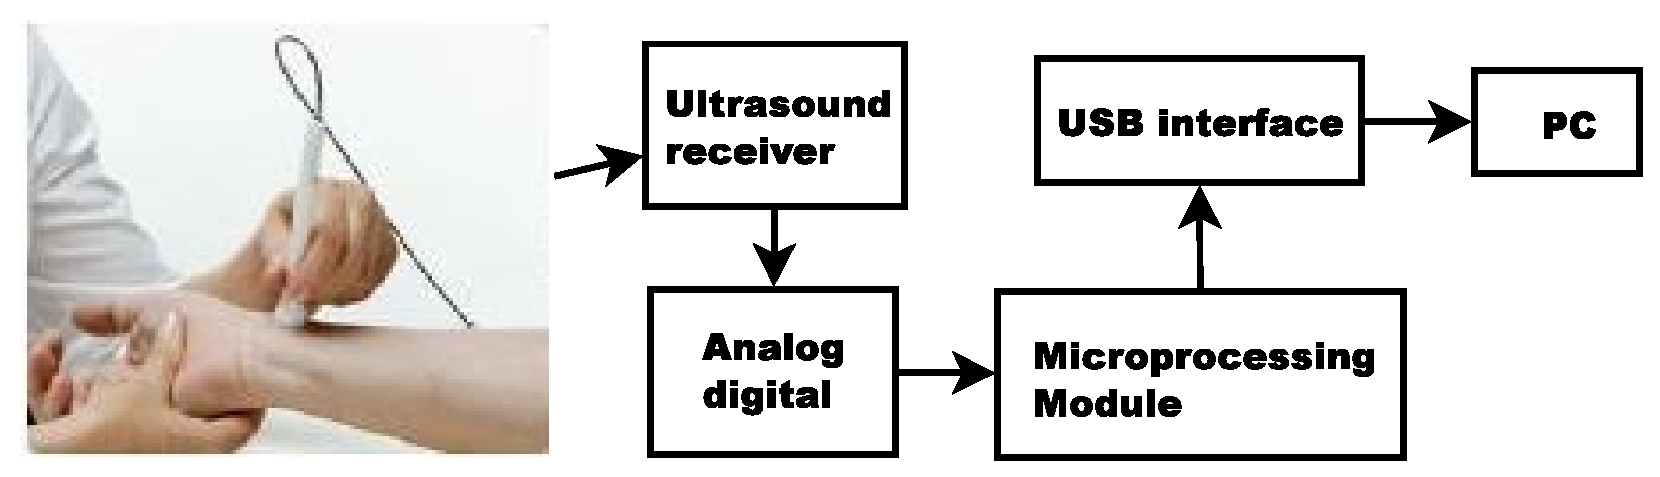
\includegraphics[width=0.7\textwidth]{ultrasound}
    \end{center}
    \caption{Pulse signal collection using ultrasonic blood analyzer}
    \label{fig:ultrasound}
\end{figure}
Aside from the diversity of sensor elements, the pattern of pulse
probes could be manifold, e.g. single position pattern, triple
positions pattern, multiple position pattern, rigid touch pattern,
soft touch pattern, in which single position pattern is the most
prevalent. Nevertheless, pulse probes trend to adopt triple positions
pattern. Multiple positions pattern or array pattern can eliminate the
accidental error from single point measurement. But how to collect and
analyze the extremely high dimentional information is still a problem.
The paper extends analysis upon pulse device with composite pressure and photoelectric
sensors. 

\subsection{The analysis and diagnosis objectified digital features}
Raw pulse data from the pulse sensors is not suitable for direct
analysis. Instead, it should be preprocessed first. The analysis of
pulse digital features mainly is separated into two steps, i.e. signal
processing and pattern classification. The signal
processing of pulse mainly solves the interference from high frequency
noise, pseudo-peaks, baseline drift, and classifies and verifies the
pulse signal by extracting feature argument from the waveform. 

Then some diagnosis features that manage to reflect the
characteristics of pulse signal are extracted, which can be
time-domain, frequency-domain features and time-frequency
features.\cite{zhang2005study,leonard2004wavelet,zhang2002wavelet, lu1999pulse,zhang2008wavelet,chen2011computerized}
 For example, Leonard et al.\cite{leonard2004wavelet} revealed that it is possible to
distinguish healthy and unwell children by using wavelet power
features and wavelet entropy of the pulse signal. Zhang et al.\cite{zhang2002wavelet}
proposed a wavelet transform based method to extract features from
carotid blood flow signals, and used a back-propagation (BP) neural
network to make the classification among 30 samples. Moreover, Zhang
et al.\cite{zhang2008wavelet} used the wavelet method to extract different pulse
features, including wavelet powers, wavelet packet powers and Doppler
ultrasonic diagnostic parameters. Although some of the above methods
have achieved encouraging results, their effectiveness are still
subject to further assessment due to the limited number of samples and
types of diseases. For example, in Leonard’s research,\cite{leonard2004wavelet} only 20
samples are used to distinguish well and unwell children, while in
Zhang’s research,\cite{zhang2008wavelet} two kinds of diseases are investigated. 

In view of the pulse research centered on linear method, nonlinear
dynamics as the third revolution of physics in this century is
gradually applied on the pulse feature extraction. At present,
nonlinear methods perform well on bio-signal to some extent for that
the human body is a nonlinear system, an integral constituted by time
and space. Consequently, a couple of methods based on nonlinear
dynamics are used to research the law of
pulse.\cite{li1999study,rauchberger1998analysis,barreto1997adaptive,naschitz2003assessment}
Wang primarily studied on the pulse mutation\cite{li1999study} and Rauchberger et al. studies on
the quotidian variation of pulse.\cite{rauchberger1998analysis} Armando et al. devised an
adapted method of plethysmography to amplify signals.\cite{barreto1997adaptive} Moreover,
Naschitz et al. used fractal and recursive graph to analyze the
transmission time of pulse.\cite{naschitz2003assessment}

When it comes to the next stage pattern classification, major methods
such as multi-factor pulse image recognition, syntactic pattern
recognition, adapted auto-regression modeling, fuzzy logic, clustering
analysis, neural network method etc. are widely used. For example,
Allen found that neural network method archived the best result
comparing with linear discriminant method and K-neighbor method. 
Chen et al.\cite{chen2009wrist} introduced Fuzzy C-Means (FCM) which aims, as a most
widely used algorithm for statistical data analysis, to cluster two or
more data point groups into clusters so that items in the same class
are as similar as possible and items in different classes are
dissimilar as possible, and found the use of membership function in
FCM that means an object can belong an object several clusters at the
same time but with different degrees is important for disease
analysis. Some other researchers\cite{zhang2005study,lu1999pulse} also proved that it is
possible to identify human sub-health status based on pulse signals by
using linear discriminate classifier. 

In summary, the research status of computerized pulse has not yet
formulated a standard to describe completely the 28 traditional pulse
types by digital features. The formation of pulse is actually so
complicated that solo sensor cannot represent the precise information
of pulse, instead fusion of multi-sensors become more effective.
Moreover, such factors as the repeatability of pulse collection, the
precise position of pulse, the pressure of probe are all basic
problems that we need solve. The established analysis of pulse image
only relies on time domain, frequency domain and simple clustering
that more incisive feature extraction method is required. Another
problem is that the objectified pulse has not been well associated
with concrete disease in clinical diagnosis. Combining with other
diagnosis method such as ECG, tongue color, oral smell makes it more
precise for prognosis as well. 

\section{Thesis organization}

Fig.~\ref{fig:outline} shows the outline of this thesis. First, pulse
data of patients with disparate health condition is gathered in
Guangdong hospital of Tradition Chinese Medicine, based
on an independent pulse detecting and collecting device with fusion of
pressure and photoelectric transducers, and then organized as the
database for later research. Second, de-noising algorithms are
introduced to detect and remove pseudo-peaks and singulars. Third, a
new series of features proposed helps the discrimination of diseases.
Finally, several classifiers are used to evaluate the
representativeness of features.

\begin{figure}[htpb]
    \begin{center}
        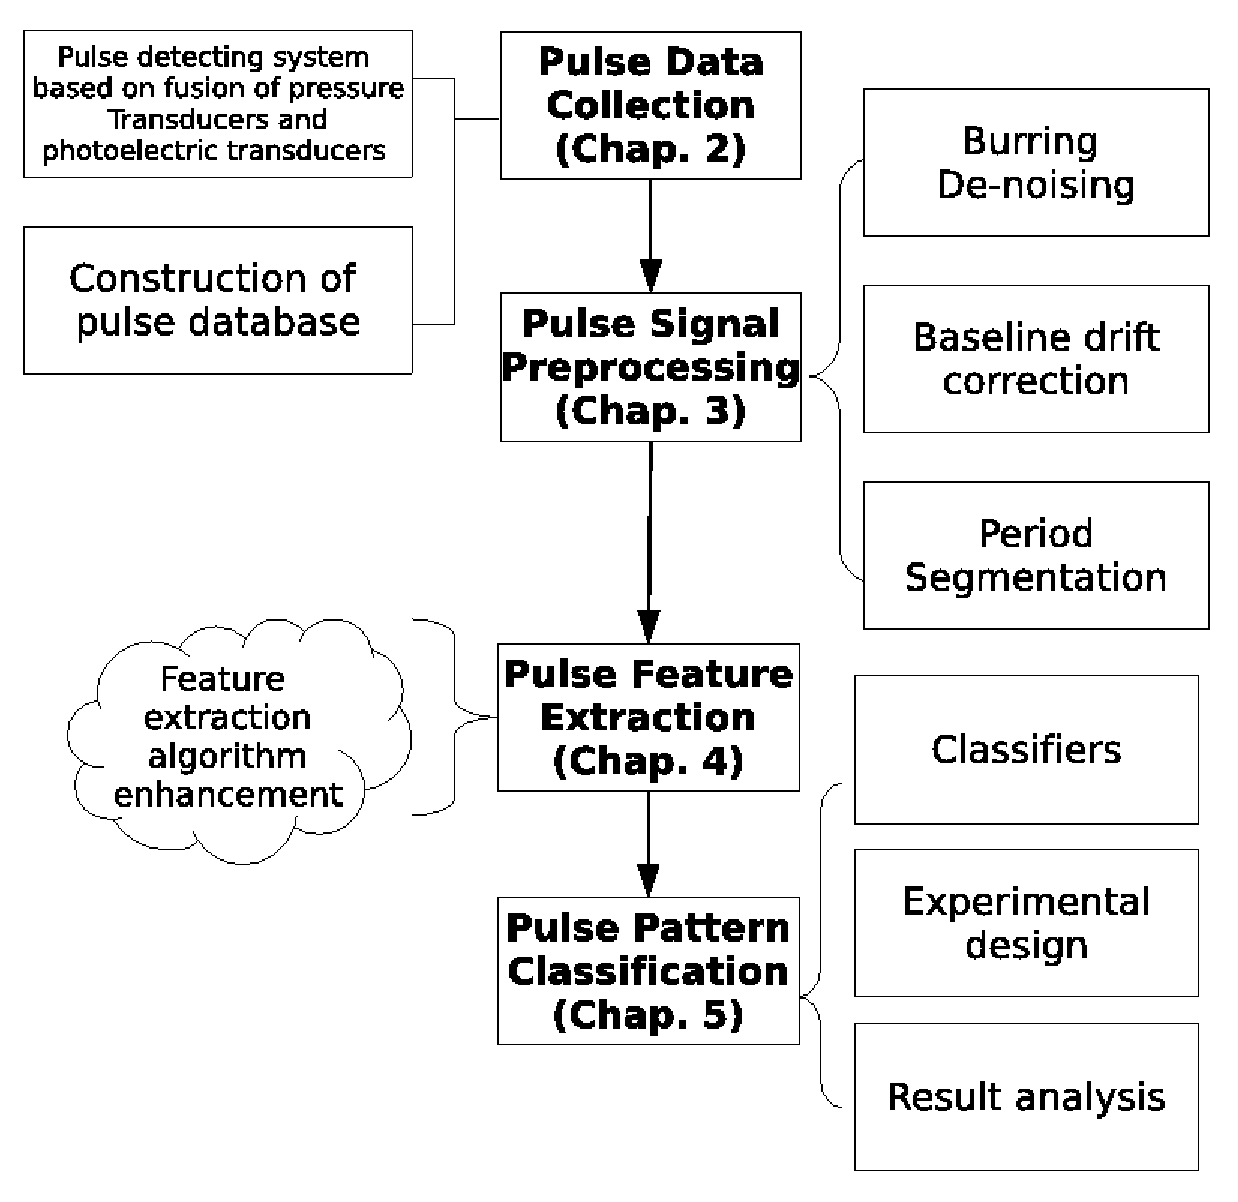
\includegraphics[width=0.8\textwidth]{outline}
    \end{center}
    \caption{Outline of this thesis}
    \label{fig:outline}
\end{figure}

The main content of the paper is organized as follows. 

Chapter~\ref{chap:one} introduces the background of pulse diagnosis
and related research status.

Chapter~\ref{chap:two} describes the principle and basic structure of pressure sensors and
photoelectric sensors based pulse collecting system, and
how to gather wrist pulse data from patients in the hospital. After
that, information is well ordered and saved as an integrated database. 

Chapter~\ref{chap:three} presents a succession of algorithms to 
remove abnormality and smooth the pulse waveforms. First, a
high-frequent burr due to the electromagnetic interference of the
device power is adulterated into the pulse signal, which urges the wavelet
1-D noise filter to smooth. Second, An unknown noise is discovered and
gotten rid of using low-pass linear filter. Third, a wavelet-based
cascaded adaptive filter helps remove the baseline drift problem
occurred during the sampling process. Finally, single periodical
waveform is cut out for further analysis. 

Chapter~\ref{chap:four} illustrates improved time-domain features and
other-domain features extracted. \todo{}

Chapter~\ref{chap:five} compares the performance of features under
three classifiers, i.e. support vector machine (SVM), Linear
Discriminant analysis (LDA), K-nearest neighbor (KNN). \todo{}

In the end, the essay makes a conclusion to summarize and evaluate the
work and addresses the prospect of pulse objectification. 



\chapter[Pulse collecting device and pulse database]{\uppercase{Pulse
collecting device and pulse database}}
\label{chap:two}

The acquisition of wrist pulse plays an crucial role in the
objectification, standardization and automation of pulse diagnosis.
Generally speaking, the quality of pulse signals obtained in the stage
has much to do with the subsequent sections, to some extent, deciding
the analysis performance of overall system. In the pulse
objectification history, pulse analytical instruments took on the
responsibility to transform human oscillation signal to visualized
images or figures easy to observe. And the designing of transducer
takes up the most part of electropulsograph development. The paper 
uses pulse collecting apparatus based on the fusion of pressure
sensors and photoelectric sensors to obtain pulse data. Then it
displays the way to collect pulse information. At last, the
construction of pulse database is explained in the paper. 

\section{Pulse collecting system}
So far, The pulse sensor has a wide range of types,
and uneven performances, which can be commonly divided into four
categories by the principle of work. One is the pressure sensor, by
detecting the pressure fluctuation at the position of radial artery
and describe the pulse image; Second is photoelectric sensor, by 
perceiving the change of vascular volume to describe the pulse information;
Third is the microphone, a sensor based on acoustics theories, in a
way to pick up the vibration caused by the pulse, i.e.
``listening'' to the signal; The last one is the ultrasonic Doppler technique.
\par 1. Pressure sensor
\par In the pressure sensor category, the piezoresistance pressure transducer
is the most widely used, which perceives the vibration of pulse on the
attribution that the resistivity changes along with the deformation
degree of medium. The attribution render the limitation that the
strain gauge must be attached on the test piece or the elastic
element in test. In the case, the performance of adhesive will
directly affect the operating feature of strain gauges (e.g.
creep deformation, mechanical lag, insulation resistance, sensitivity,
nonlinearity) and the extent of changes of these features over time or
temperature. Consequently, it restricts the accuracy, linearity and the scope
of application to the strain pressure sensor.
\par 2. Photoelectric sensor 
\par Here is its detection principle: Fluctuations in blood flow
cause the change of blood volume per unit, and the amount of blood
volume decides the portion of the light absorbed by blood. So when the
light is cast on the tissue, the amount of light reflected varies with
the fluctuation of blood flow. Finally the photoelectric transducer
converts the optical signal into electrical signal to reflect the change
of pulse waveform. 

The photoelectric transducer implements photoelectric
isolation, reducing interference to the next level of analog
circuit. Hence, it has high anti-jamming capacity, high sensitivity, 
good linearity and frequency response characteristic. Due to
insufficient acknowledgement to the internal connection between the vascular volume
and pulse information, only two indicators oxygen and pulse rate
can not meet the need for other blood stream arguments. 
\par 3. Microphone
\par The research in recent years shows wrist pulse signal is
naturally a kind of infrasonic wave, a vibration transmitting over the
special medium radial artery. Binghe Wang et al. adopted indirect
coupling (i.e. non-contact) extraction method to acquire the spectrum
characteristic of PingMai and XuanMai. An air column is set up to couple the
acoustic wave produced by vibration of wrist pulse.~\cite{B.1998}
\par 4. Ultrasonic Doppler technique
\par Besides the pressure information, arterial pulse includes lumen volume, blood flow
rate, three-dimensional vascular motion and other information. The
solo pressure factor hardly reflects the indicator of each component
in pulse. With the development of medical ultrasonic imaging technology, 
the application of ultrasound Doppler technique keeps its pace on the
objectification of pulse image. DongYu Zhang et al. extracted pulse
signal in the form of envelope line from the ultrasonic
image.~\cite{zhang2008wavelet} 

Although microphone and ultrasonic Doppler technique could receive
more information, the principle betrays the traditional pressing type
sphygmotechny. So the both hardly reflect the features of pulse
correctly.

The pulse collecting apparatus adopted in the subject is jointly
developed by Harbin Institution of Technology and HongKong PolyTechnic
University. See Figure~\ref{fig:device}. In the light of a better simulation of fingertips-touch
pulse diagnosis than the other sensors and its more convenient way of
fixation and pressurization, the pressure sensor is preferred. For
comparison purpose, photoelectric sensors are also built in the probe.
Therefore, the system contains 9 photoelectric transducers and one
pressure sensor in each position, totally 30 sensors. The upper screws
are used to increase pressure. The probe is shown in
Figure~\ref{fig:probe}. 

The pressure sensors and photoelectric transducers convert pulse
signal to analog electric signal. Then the signal is optimized in the
signal processing module, transformed in A/D converter and saved in
computer via USB line. 
\begin{figure}[htbp]
    \centering
    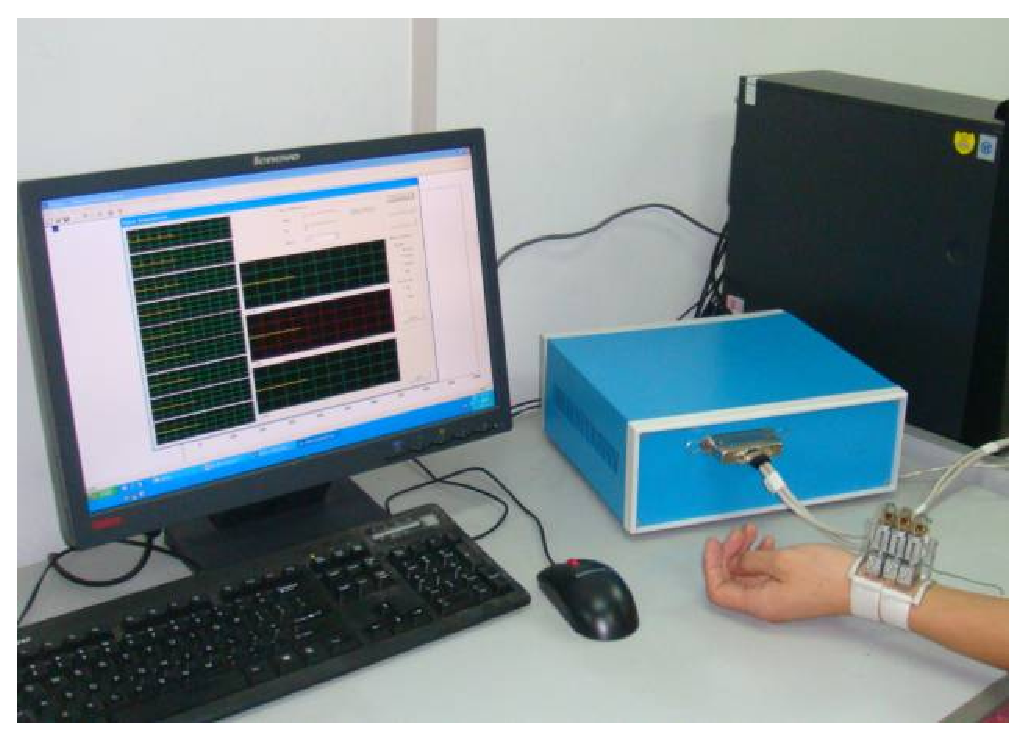
\includegraphics[width=0.6\textwidth]{device}
    \caption{Pulse collecting system}
    \label{fig:device}
\end{figure}
\begin{figure}[htbp]
    \centering
    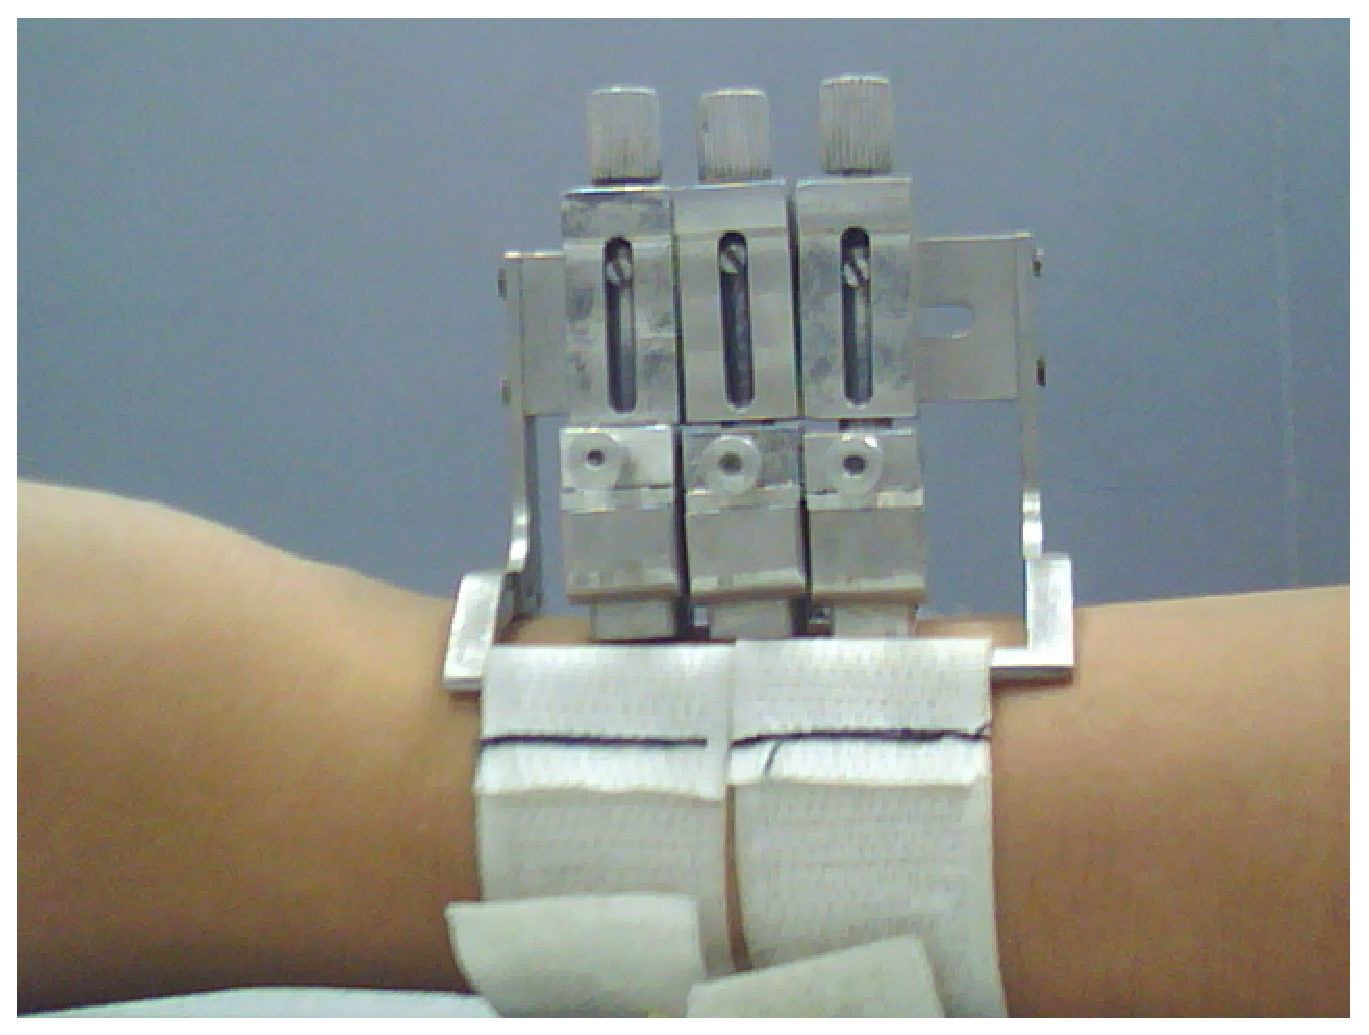
\includegraphics[width=0.6\textwidth]{probe}
    \caption{Probe head: fusion of photoelectric sensors and pressure sensors}
    \label{fig:probe}
\end{figure}
The biological signal of human body is a kind of continuous time
signal, which is difficult to process in computer. Therefore, the
pulse collecting apparatus fulfills this task and transmits
digital signals to computer. However, the overall process may loss a
certain amount of information. In other words, the digitalized signal
losses part of information during conversion. That is what 
The theorem describes two processes in signal processing: a sampling
process, in which a continuous time signal is converted to a discrete
time signal, and a reconstruction process, in which the original
continuous signal is recovered from the discrete time signal.
According to Nyquist theorem, the sampling frequency must be at least 
twice the highest frequency contained in the signal, or in
mathematical terms:
\begin{equation}
    f_s \geq f_e
    \label{eq:nyquist}
\end{equation}
where $f_s$ is the sampling frequency (how often samples are taken per
unit of time or space), and $f_e$ is the highest frequency contained
in the signal. So our device sets default frequency as 500Hz so as to
capture more details.  

The system is redesigned based on the model of first generation pulse
detecting system made by Harbin Institution of Technology. See
Figure~\ref{fig:1stgen}. Compared with the first generation system,
the new system has the following advantages:
\begin{enumerate}[(1)]
    \item Acquire more information. The pulse length and pulse width
        could be obtained. 
    \item Plug-and-play. The system reaps the benefits of USB 2.0
        which makes devices easy to use.
    \item Locate function. The photoelectric sensor array helps
        practitioners quickly locate the right position of radial artery. 
    \item Modularized design. Six independent modules, i.e. sensors, analog
        circuits, digital circuits, firmware, driver and application,
        reduce the probability to break down and let improvement and
        maintenance easier.
\end{enumerate}
\begin{figure}[htpb]
    \begin{center}
        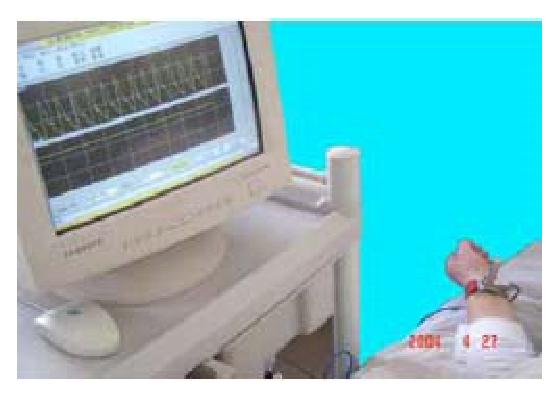
\includegraphics[width=0.8\textwidth]{1stgen}
    \end{center}
    \caption{The first generation of pulse detecting system developed
    by Harbin Institution of Technology}
    \label{fig:1stgen}
\end{figure}

In spite of the advantages described above, the system still exposed
a few deficiencies listed as follows: 
\begin{enumerate}[(1)]
    \item Poor durability. In pulse collection period, four or five
        continuous working seems common. Unfortunately, some sensors
        malfunction as sudden with the result that signals on those channels
        remain null. So the incompleteness of signal information brings
        trouble to the further analysis. 
    \item Unstable. The pressure value often drifts unexpectedly
        during collection. Normally it wanders around 200g, but
        sometimes it jump to 7000g, that is impossible. Probably the
        bug occurs in the strain gauge. In addition, it is hard to
        keep the same of pressure values on three positions. 
    \item Bad operability. During actual manipulation, even skilled
        practitioners fail to ensure all three positions detect
        signals. The three probe heads relates each other that
        adjustment on one probe head may displace others. 
\end{enumerate}

\section{The collection of wrist pulse}
It is worth to explain the detail of pulse collecting process for the
sake of understanding the simulation of pulse diagnosis via
automated apparatus. 
\par 1. Record personal information 
\par As is known to all, lung, spleen, liver and
kidney are all basic entrails as well as heart to maintain the
body functions. The diversity of morphological structures and
physiological characteristics to these entrails generates the
corresponding the five internal organs. Besides, in view of the tight
relationship of entrails with heart, pulse, Qi in TCM, blood, the
interaction and coordination among them has influence on pulse shape.
Moreover, the wrist pulse may vary due to the change of mental health
even though the physical organs work well. Hence, before the
collection, the biological indexes (e.g. gender, age, height, weight)
are also needed as a reference approach. A person information
management dialog is designed in view of convenience
shown as Figure~\ref{fig:dialog}.
\begin{figure}[htpb]
    \begin{center}
        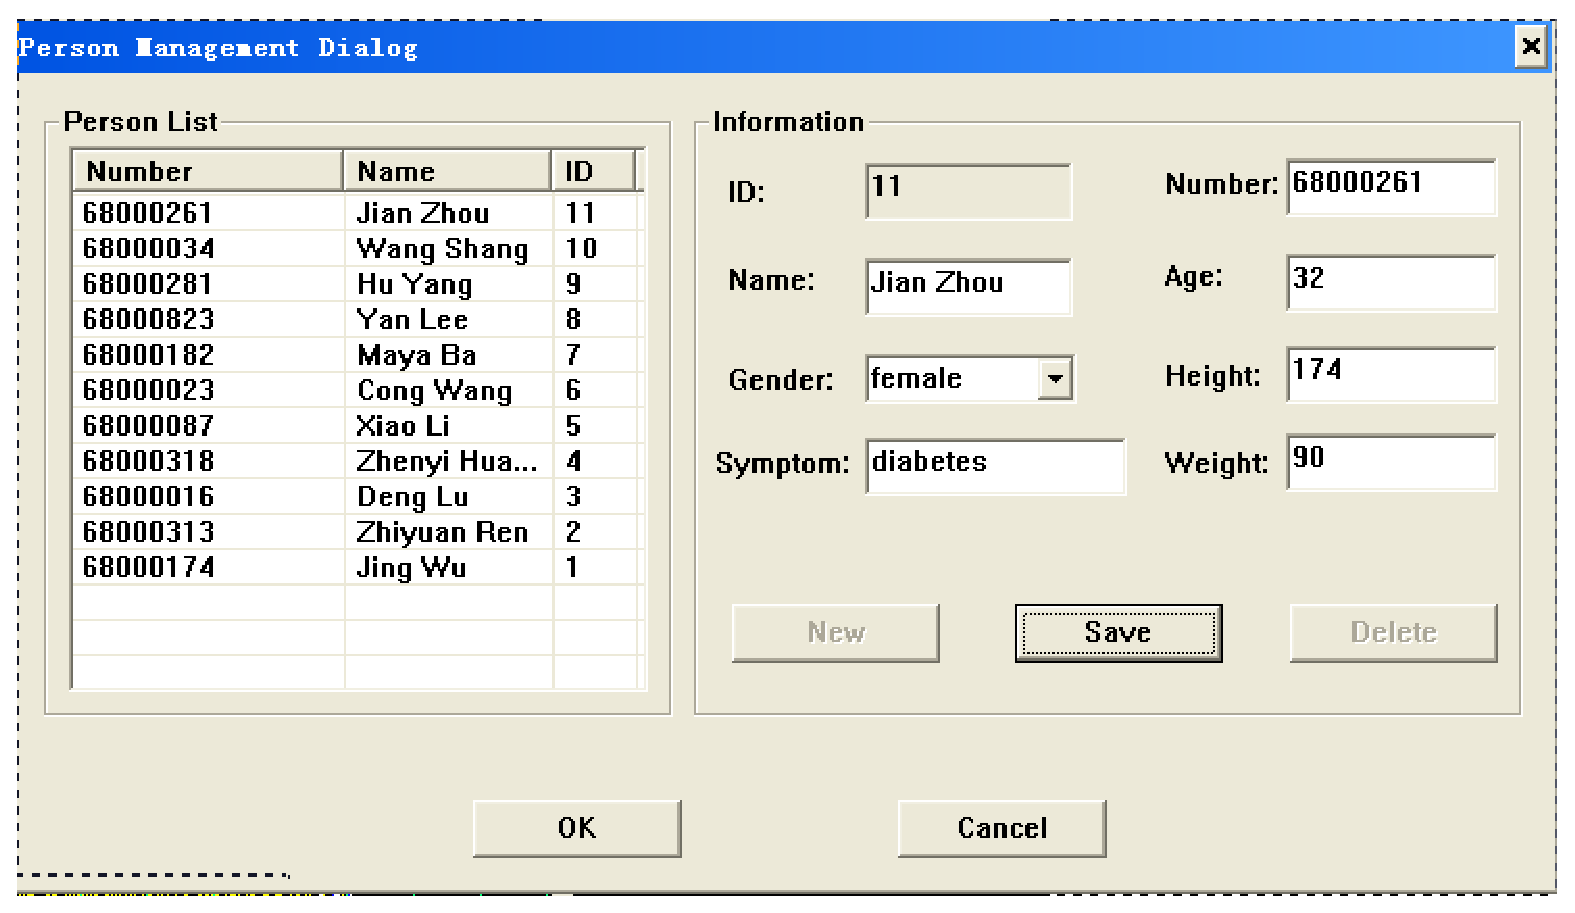
\includegraphics[width=0.9\textwidth]{dialog}
    \end{center}
    \caption{Person management interface}
    \label{fig:dialog}
\end{figure}
\par 2. Hand selection
\par In TCM pulse diagnosis, the practitioners usually use three fingertips (Index,
Middle and Ring fingers) to touch the left hand of patient and feel
the pulse fluctuation on three positions, i.e. `Cun', `Guan' and
`Chi'. Hence, in order to best simulation, the left hand is selected
in this experiment.
\par 3. Wrist pulse detecting process 
\par  The signal collection process includes usually three
steps. 
\begin{enumerate}[(1)]
    \item Find a rough location in the wrist. The
    practitioners use the three fingertips mentioned above to feel the
    proper position of the wrist (the experiment adopts the left
    hand) to place the probe. Generally speaking, the practitioner
    should ensure the probe detect signals on each position. 
    \item Fine tune and observation. 
        Take the Guan part as example. There are nine photoelectric
        sensors in the part. If the intensity of signals detected
        on one side are much stronger than the other side, then 
        it indicates that the sensor should be slightly fine-tuned
        towards the weak side. It also works to other two positions.
    \item Repeat the foregoing steps until signals from three points
        are observable, including pressure sensors and photoelectric
        sensors. See Figure~\ref{fig:interface}.
    \item Adjust pressure value. The paper imitates the process of 
        pulse diagnosis to feel the intensity of radial artery signals 
        in different pressure values. By manually twisting the screw
        of probe, pressure value to the radial artery could change. 
        Figure~\ref{fig:pressure} shows the intensity divergence of pulse
        signals under 130g, 200g, 250g pressures. The amplitude
        increases by \hl{1.8} when
        the pressure increases from \hl{130} to \hl{200g}
        while the amplitude yet decreases by about \hl{0.5} when the
        pressure value increases from \hl{200g} to \hl{250}.
        Therefore, the pressure value is considered as the best value to
        show the pulse obtained.
    \item Record 2-3 records. Each record should last at least 10
        seconds. During the sampling period, no laughing and talking
        is allowed. 
\end{enumerate}
\begin{figure}[htpb]
    \begin{center}
        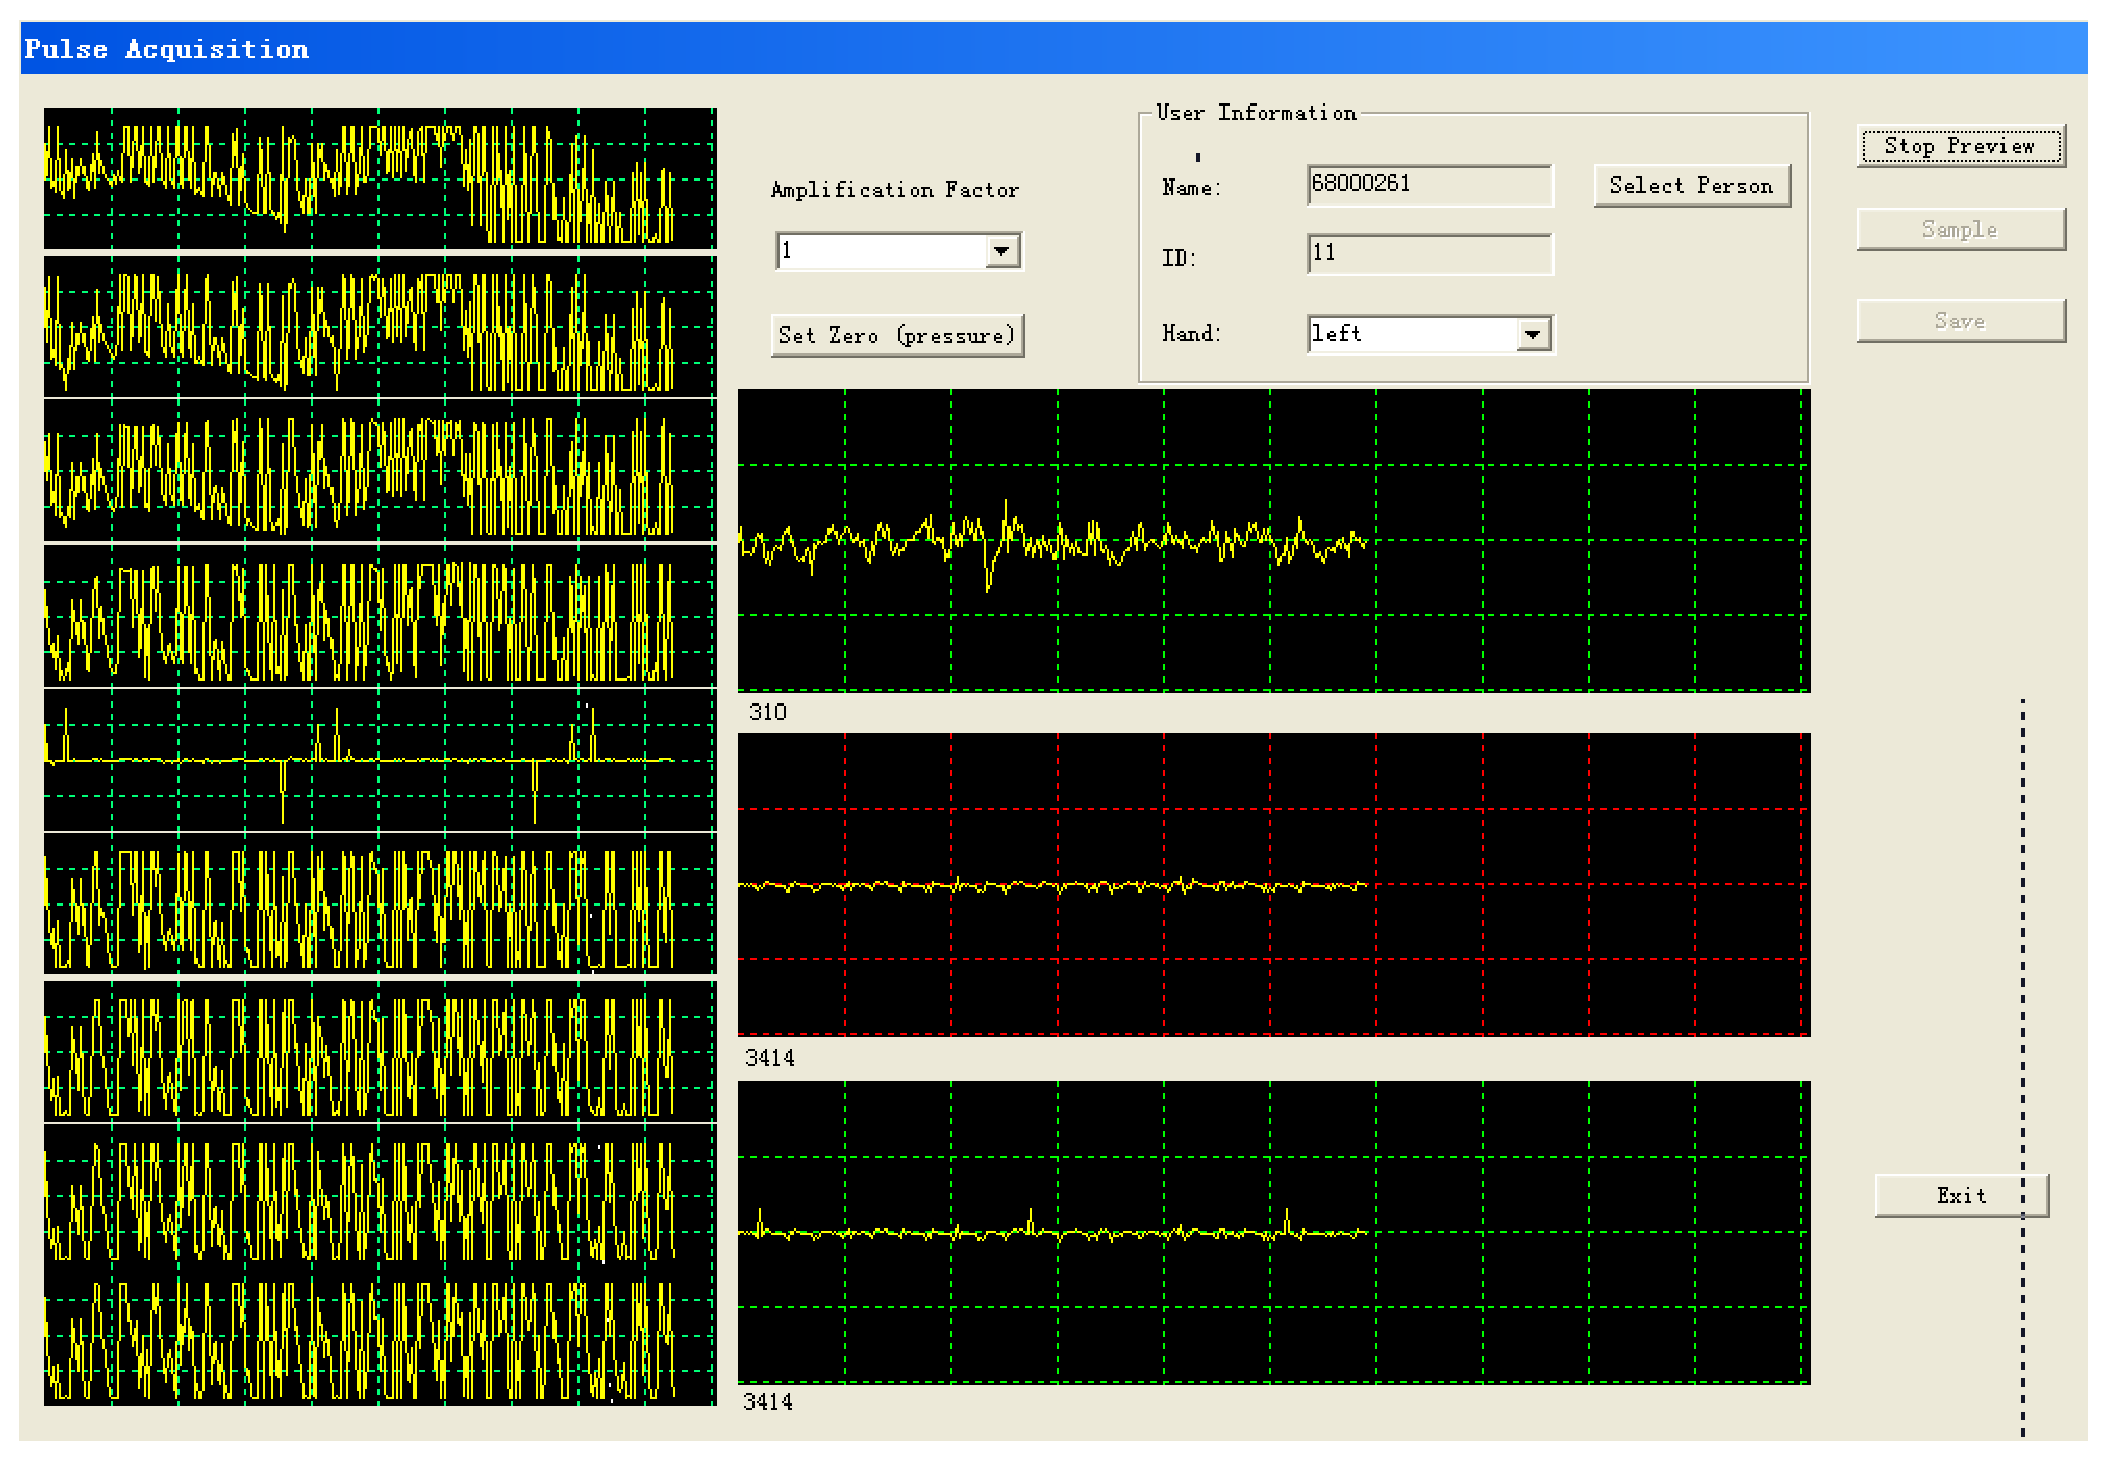
\includegraphics[width=0.7\textwidth]{interface}
    \end{center}
    \caption{Main interface for pulse collection}
    \label{fig:interface}
\end{figure}

\begin{figure}[htbp]
    \centering
    \subfloat[Pulse signal when the pressure is
    130]{\label{fig:130g}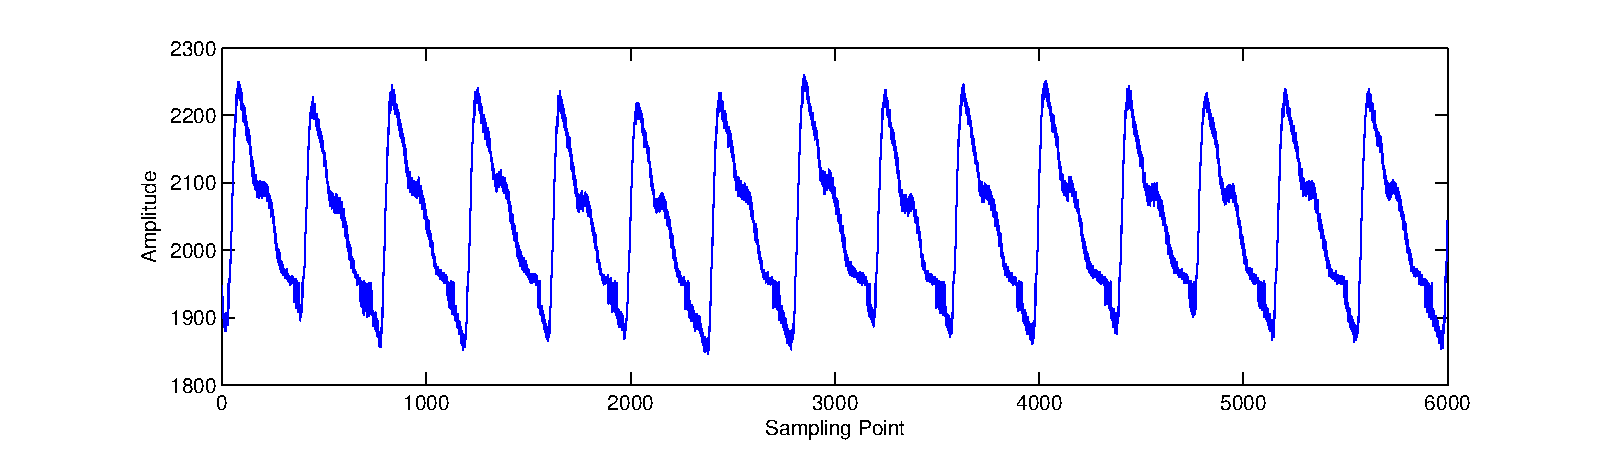
\includegraphics[width=0.7\textwidth]{130g}}\\
    \subfloat[Pulse signal when the pressure is
    200g]{\label{fig:200g}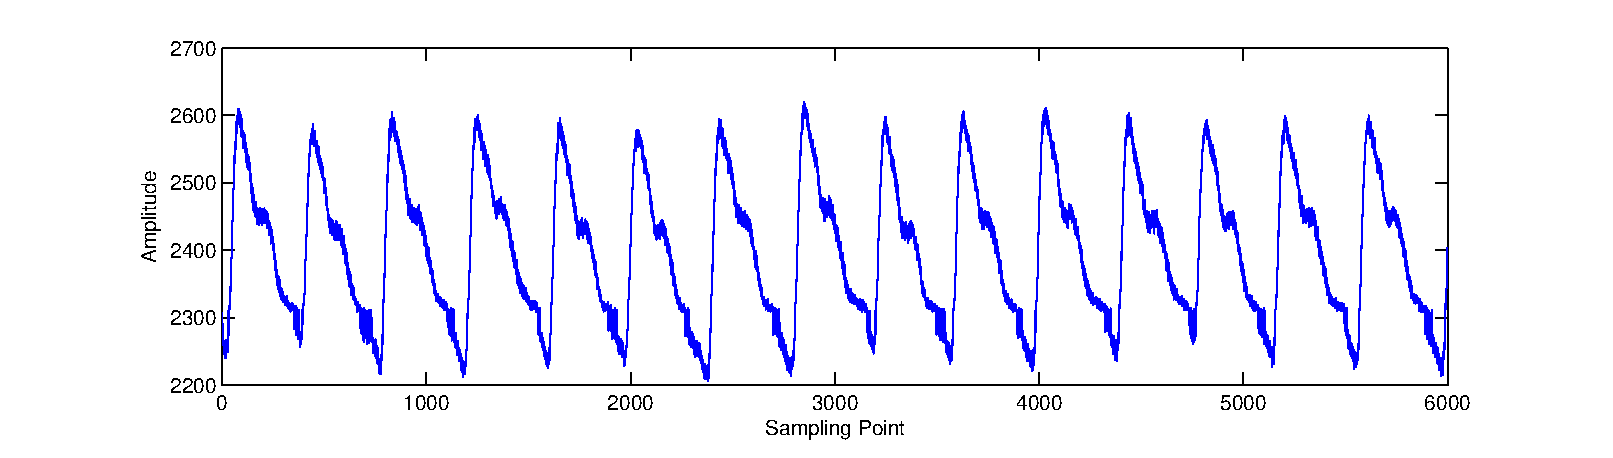
\includegraphics[width=0.7\textwidth]{200g}}\\
    \subfloat[Pulse signal when the pressure is
    250g]{\label{fig:250g}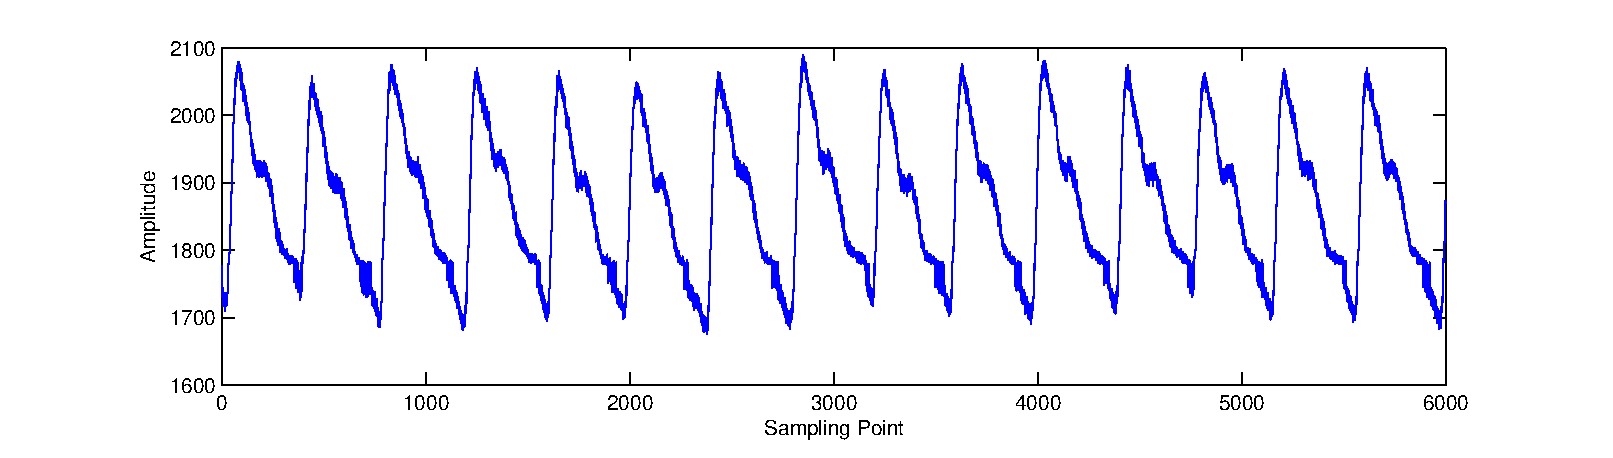
\includegraphics[width=0.7\textwidth]{250g}}\\
    \caption{Pulse signals under three different pressures}
    \label{fig:pressure}
\end{figure}

\section{Pulse database}
After a month of pulse data acquisition, the team has collected 
in total 2247 samples, in which 1565 ones are from physical
examination section and 682 ones are from wards. All the samples are
from Guangdong Hospital of TCM. Table~\ref{tab:database} shows the
main portion of database used in the following chapters. Other sets of
data are either too few in number or information insufficiency. 
The 1565 health examinees are mostly 30 to 40 years old while the rest
682 patients range from 16 to 70 of age. The class of samples results from
western medicine diagnoses provided by the hospital. \todo{再多写一点}
\begin{table}
    \centering
    \begin{tabular}{cc}
        \toprule[1.5pt]
        Disease & Number \\
        \midrule[1pt]
        healthy & 150 \\
        subhealthy & 879 \\
        gastrosia & 28 \\
        nephrosis & 54 \\
        diabetes & 54 \\
        respiratory disease & 33 \\
        angiocardiopathy disease & 35 \\
        endocrine disease & 70 \\
        cardiology & 15 \\
        \bottomrule[1.5pt]
    \end{tabular}
    \caption{Main part of database}
    \label{tab:database}
\end{table}

\section{Summary}
The chapter first introduced four typical sensors: pressure sensor,
photoelectric sensor, microphone, ultrasonic Doppler sensor. The pulse
collecting system in the paper utilized pressure sensor and
photoelectric sensor. In three positions, `Cun', `Guan', `Chi', there
is a probe head which perceives 9-channel photoelectric pulse signals
and one pressure pulse signal. Second, it introduced the advantages and
disadvantages of the system. Third, the paper described the entire collecting
process. The quality of pulse data gathered binds the later
performance of classification. Finally, a pulse database is
established with the pulse information of thousands of people. 
In summary, the automated pulse diagnosis system, to which is widely
payed attention, has important application value. 
Therefore, it significantly makes sense to adopt a exceptional
pulse collecting system to gather accurate pulse information 
and establish a database of rich personal physical information. 


\chapter[Pulse signal preprocessing]{\uppercase{Pulse signal preprocessing}}
\label{chap:three}

Owing to the electromagnetic interference in surrounding environment,
high frequency noise will be superimposed on the original signal
amid collection, affecting the signal analysis. 
Meanwhile, the breathing or body movement of participant will also
cause the signal baseline drift. Distortion of pulse features
extracted would probably occur afterwards unless the baseline drift problem
was solved. Therefore, the both problems must be properly handled
towards the original pulse signal. In addition, since the subsequent
pulse feature extraction is based on a single period of pulse
waveform, a period segmentation algorithm fulfills the task to split
signal series. The chapter employs wavelet transform to filter
high-frequency noise, wavelet-based cascaded adaptive filter to remove
baseline drift, and a period detection algorithm to divide periods.
At last, the pulse waveform is normalized.
Figure~\ref{fig:preprocessing} demonstrates the outline of this
chapter.
\begin{figure}[htpb]
    \begin{center}
        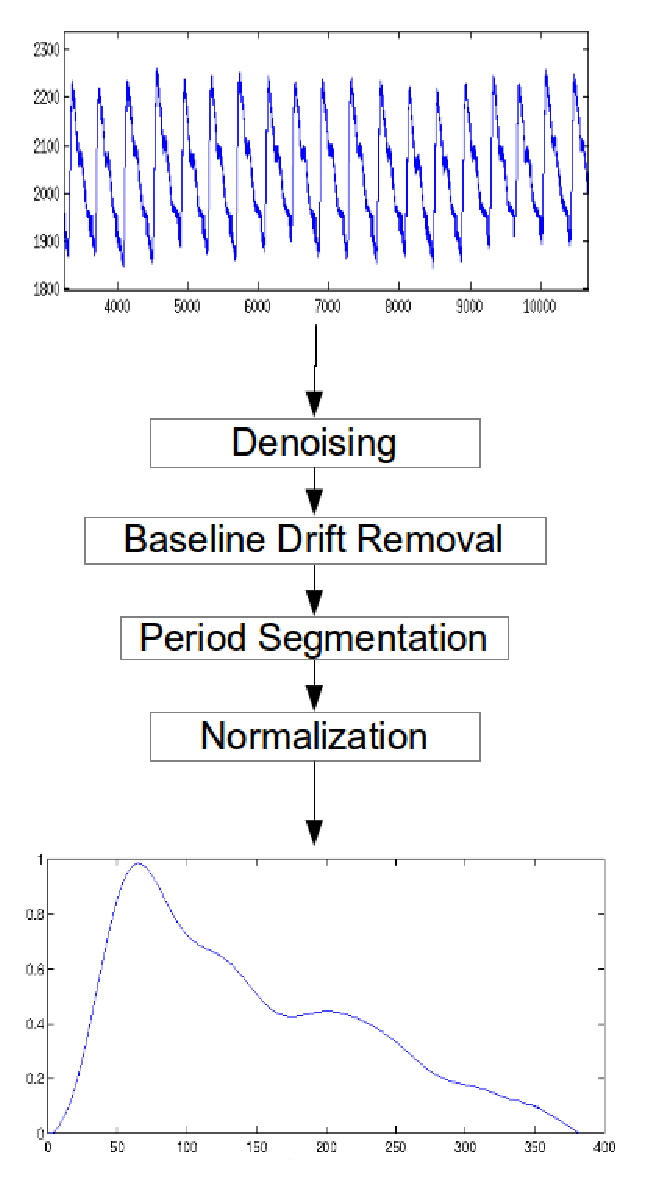
\includegraphics[width=0.4\textwidth]{preprocessing}
    \end{center}
    \caption{Preprocessing procedures}
    \label{fig:preprocessing}
\end{figure}



\section{Burring}
The human wrist pulse signal is a weak physiological signal that
is susceptibly to high-frequency noise caused by interference of
electromagnetic devices. This sort is called \emph{burr} because the
noise looks like small notches in the fringe of objects. See
Figure~\ref{fig:beforeburr}. 
\begin{figure}[htpb]
    \begin{center}
        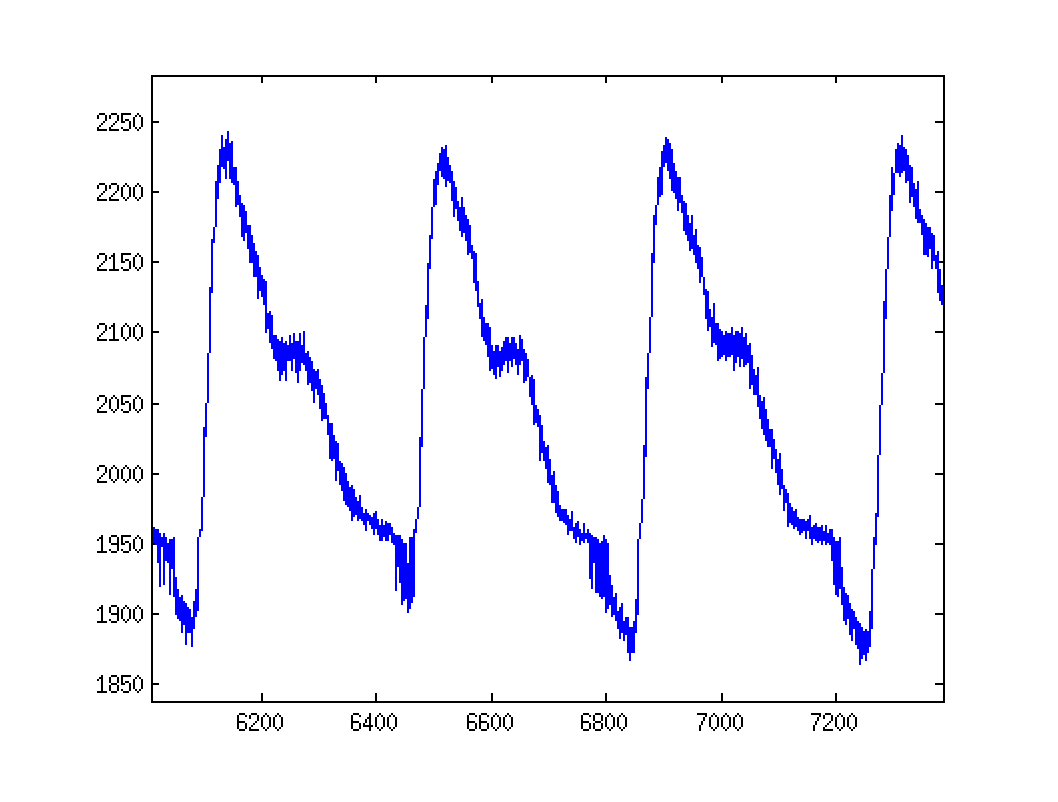
\includegraphics[width=0.7\textwidth]{beforeburr}
    \end{center}
    \caption{Pulse signal with burr noise}
    \label{fig:beforeburr}
\end{figure}
By careful observation, the burrs in pulse signals present a jagged
form in overall, which means glitches float uniformly around the real
value. In actual processing, the majority of signals may contain
spikes or mutation, and the noise signal is not stable white noise yet. 
So does the pulse signal. Fourier transform based spectral analysis is
the dominant analytical tool for frequency 
domain analysis. However, Fourier transform cannot provide any
information of the spectrum changes with respect to time.  Fourier
transform assumes the signal is stationary, but pulse signal is always
non-stationary. The traditional Fourier transform 
considers information merely on frequency-domain and becomes powerless
to differentiate the change on a specific point. Admittedly, the
traditional Fourier low pass filter could suppress the noise, it
meanwhile blurs the noisy edge of one-dimension signal. If the
low-pass frequency range is narrow, high-frequency components of the
mutation part will be treated as noise to be filtered,
which led to a certain amount of distortion in the mutation part; If
the range of low-pass frequency is set too wide, the noise may not be
effectively filtered out. To overcome this deficiency, a modified method-short
time Fourier transform allows to represent the signal in both time and
frequency domain through time windowing function. The window
length determines a constant time and frequency resolution. Thus, a
shorter time windowing is used in order to capture the transient
behavior of a signal; we sacrifice the frequency resolution.
So, an alternative mathematical tool- wavelet
transform must be selected to extract the relevant time-amplitude
information from a signal.  In the meantime, we can improve the signal to noise ratio based on
prior knowledge of the signal characteristics. 

\subsection{Wavelet-based denoising}
Wavelet transform is a inheritance and development of Fourier
transform, that not only has a profound and comprehensive theory, 
but also emerges its wider application prospect. As is known to
everyone, a $\Psi(t)$ is called a \emph{Mother Wavelet} if it meets
the following condition: 
\begin{equation}
    C_\Psi=\int_R \frac{|\Psi(\omega)|^2}{|\omega|}\mathrm{d}\omega <
    \infty, \quad \mathrm{for} \; \Psi \in L^2(R)
    \label{waveletdefinition}
\end{equation}
Do a scaling and shifting operation to the mother function as 
\begin{equation}
    \Psi_{a,b}(t) = |a|^{-\frac{1}{2}}\Psi(\frac{t-b}{a}), \quad b \in
    R, \, a \in R - \{0\}.
    \label{waveletbase}
\end{equation}
Then The function family ${\Psi_{a,b}(t)}$ is called \emph{wavelet base},
where $a$ is the scale parameter and $b$ is the shift parameter. If
$a=2^j,b=k\cdot 2^j,\,j,k \in Z$, then
\begin{equation}
    \Psi_{j,k}(t)=2^{-\frac{j}{2}}\Psi(2^{-j}t-k).
    \label{wavelet3}
\end{equation}
If $\Psi(t)$ is properly chosen, ${\Psi_{j,k}(t)}$ could consist of a
family of orthonormal wavelet bases. So any function $f(t)\in L^2(R)$ can
be expanded in the form of orthonormal wavelet series:
\begin{equation}
    f(t)=\sum_{j,k=-\infty}^{+\infty} c_{j,k}\Psi_{j,k}(t)
    \label{waveletdecomp}
\end{equation}
where $c_{j,k}=<f,\Psi_{j,k}>$. The important information of signal
$f(t)$ disperses into each layer. It helps people handle specifics of
signals more conveniently from both time and space. 

One important application of wavelet transform is signal denoising.
The wavelet can efficiently remove noise on account of its good 
locality in both time-domain and frequency-domain. It could 
distinguish the mutation part and noise of signals and successfully
achieve the elimination of noise for non-stationary signals. In
essence, the wavelet transform carries out the function to depress the
useless part of the signal and intensify the useful part at the same
time.~\cite{debnath2002wavelet, Changfa2001, Qiwen2001}. 

Therefore, the paper will give priority to employ the one-dimension
wavelet transform to smooth the pulse signal. The wavelet
transform denoising process usually is divided into 3 steps~\cite{polikarwavelet}:
\begin{enumerate}[(1)]
    \item Apply wavelet transform to the noisy signal to produce the
        noisy wavelet coefficients to the level which we can properly
        distinguish the PD occurrence.
    \item Select appropriate threshold limit at each level and
        threshold method (hard or soft thresholding) to best remove
        the noises.
    \item Inverse wavelet transform of the thresholded wavelet
        coefficients to obtain a denoised signal. 
\end{enumerate}
Of the three steps, the most critical point is how to choose the
threshold and the corresponding quantification. To some extent, it
has a bearing on the effect of signal denoising. The detailed denosing
process based on wavelet transform aiming at pulse signal is shown as
below: 
\subsubsection{Wavelet selection}
Wavelet transform is essentially a description of signal features within
the space composed of a group of wavelet mother functions. The mother
function plays a critical role in wavelet transform. To best
characterize the spikes in a noisy signal, we should select our
``mother wavelet'' carefully to better approximate and capture the
transient spikes of the original signal. ``Mother wavelet'' will not
only determine how well we estimate the original signal in terms of
the shape of the PD spikes, but also, it will affect the frequency
spectrum of the denoised signal. There are seven factors needed to
consider for better choice\cite{xin2003fan}. 
\begin{enumerate}[(1)]
    \item Regularity. It is very important to obtain a smoother effect
        for reconstruction of the signal. Generally speaking, the
        more orthogonal, the better denoising effect it will reach.
    \item Compact support and attenuation. These are two important
        attributes of wavelet. In general, a wavelet will have a
        better localization capacity if it attenuates quicker. And the
        compact support of wavelet base is expected in time-domain.
    \item Symmetry. Symmetric or antisymmetric scaling function and
        wavelet function could construct compactly supported
        orthogonal wavelet base with linear phase characteristic. 
    \item Vanishing moment property. In most situations it is useful
        to restrict $\Psi$ to be a continuous function with a higher number
        $M$ of vanishing moments, i.e. for all integer $m<M$
        \begin{equation}
            \int_R t^m \Psi(t) \mathrm{d}t=0
            \label{waveletvanish}
        \end{equation} 
        It has been proved that a wavelet with high enough vanishing
        moment could effectively detect the singular point.
    \item The time-frequency window and its area. The smaller the
        window size is, the stronger the localization capacity is
        achieved. Since the time-domain window and frequency-domain
        window is resizable, the wavelet could analyze signals adaptively. 
    \item Linear phase property. Linear phase is a property of a filter, where
        the phase response of the filter is a linear function of
        frequency, excluding the possibility of wraps at $\pm\pi$. 
        In signal processing, the scaling function and wavelet can be
        thought of as filter function since a filter with linear phase
        property or generalized linear phase at least is able to avoid
        the distortion during decomposition and reconstruction. 
\end{enumerate}

On consideration of the wavelet features above and the periodicity,
the paper chooses wavelet base $sym8$ as the filter. 

\subsubsection{Level of decomposition}
From the previous section, we have known the wavelet transform is
constituted by different levels. The maximum level to apply the
wavelet transform depends on how
many data points contain in a data set, since there is a down-sampling by 2 operation
from one level to the next one. In general, there is no solid criteria.
However, the following formula helps quickly decide the
number of decomposition level~\cite{liu2004compression}:
\begin{equation}
    J=int[log_2(f_s / f_f) -1]
    \label{waveletlevel}
\end{equation}
where $f_s$ denotes the sampling frequency (500Hz in this paper),  
$f_f$ denotes the fundamental frequency (within 10Hz in this paper),
and $int$ indicates to choose round number. Consequently, 5 levels
would be proper. 

\subsubsection{Threshold limits and denoised result}
The choice of the threshold is a
very delicate and important statistical problem.  On the one hand, a
big threshold leads to a large bias of the estimator. But on the other
hand, a small threshold increases the variance of the smoother.
Many methods for setting the threshold have been proposed. The most time-consuming
way is to set the threshold limit on a case-by-case basis. The limit
is selected such that satisfactory noise removal is achieved. But in
order to achieve a better denosing effect, it had better try different
cases of thresholds. There are usually three types of threshold. 
\begin{enumerate}[(1)]
    \item Hard thresholding. For one-dimension signal, the empirical
        threshold is calculated as 
        \begin{equation}
            t=sqrt{2\sigma^2 log(n)/n}
            \label{wavelethardthreshold}
        \end{equation}
        where $n$ is the length of the input signal and $\sigma^2$ is
        the variance of the noise. The variance of the noise is
        estimated based on the data. It is done by averaging the
        squares of the empirical wavelet coefficients at the highest
        resolution scale. Hard thresholding sets any coefficient less
        than or equal to the threshold to zero. 
    \item Soft thresholding. The only difference between the hard and
        the soft thresholding procedures is in the choice of the
        nonlinear transform on the empirical wavelet coefficients. For
        soft thresholding the following nonlinear transform is used: 
        \begin{equation}
            S(x)=\mathrm{sign}(x)(|x|-t)I(|x|-t),
            \label{waveletsoftthreshold}
        \end{equation}
        where $t$ is a threshold.  Adaptive thresholding.The threshold
        is subtracted from any coefficient that is greater than the
        threshold. This moves the time series toward zero. 
    \item Adaptive thresholding. The threshold selection rule is based on
        Stein's unbiased estimate of risk(quadratic loss function).
        One gets an estimate of the risk for a particular threshold
        value $(t)$. Minimizing the risks in $(t)$ gives a selection
        for the threshold value.
\end{enumerate}

The Figure~\ref{fig:threshold} shows the comparison of denoised
signals using the three thresholds described above. From the figures,
the soft thresholding method efficiently removes the high frequency
noise and preserves the original useful information; The hard
thresholding method still leaves out much noise not filtered; The
Adaptive thresholding method fails to work properly, probably in
account for its unsuitable application for this kind of noise.
\begin{figure}
  \centering
  \subfloat[The denoised signal using hard
  threshold]{\label{fig:hard}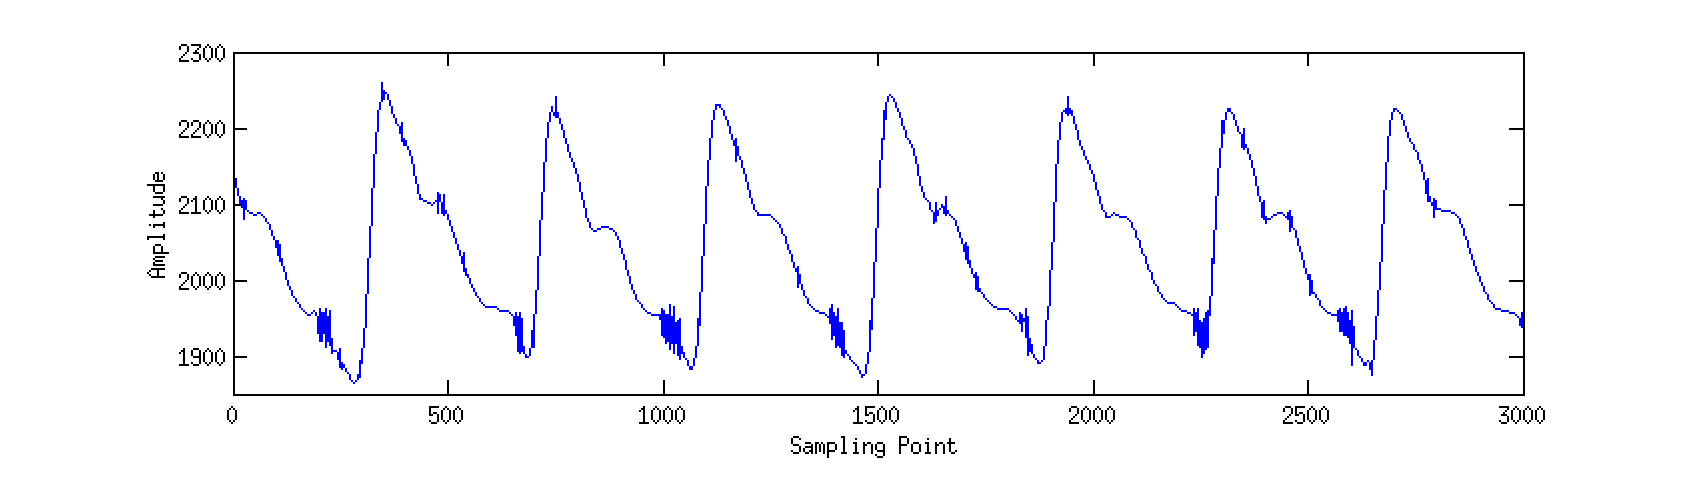
\includegraphics[width=0.9\textwidth]{hard}}\\
  \subfloat[The denoised signal using soft
  threshold]{\label{fig:soft}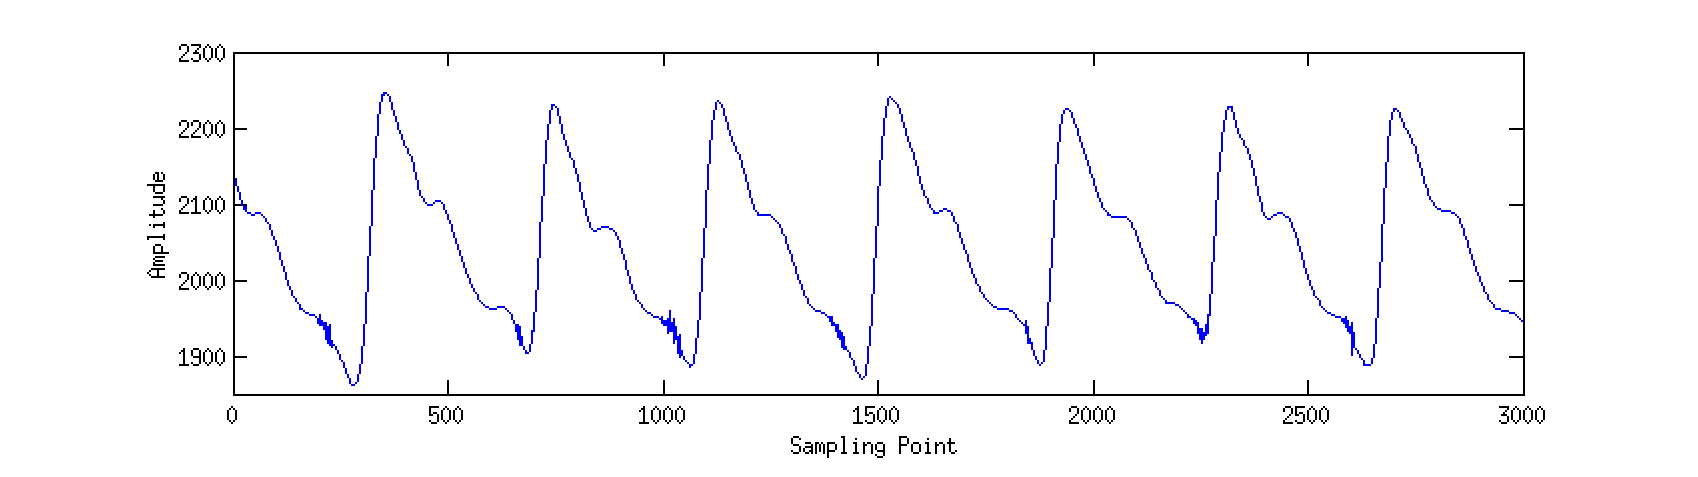
\includegraphics[width=0.9\textwidth]{soft}}\\
  \subfloat[The denoised signal using adaptive
  threshold]{\label{fig:adaptive}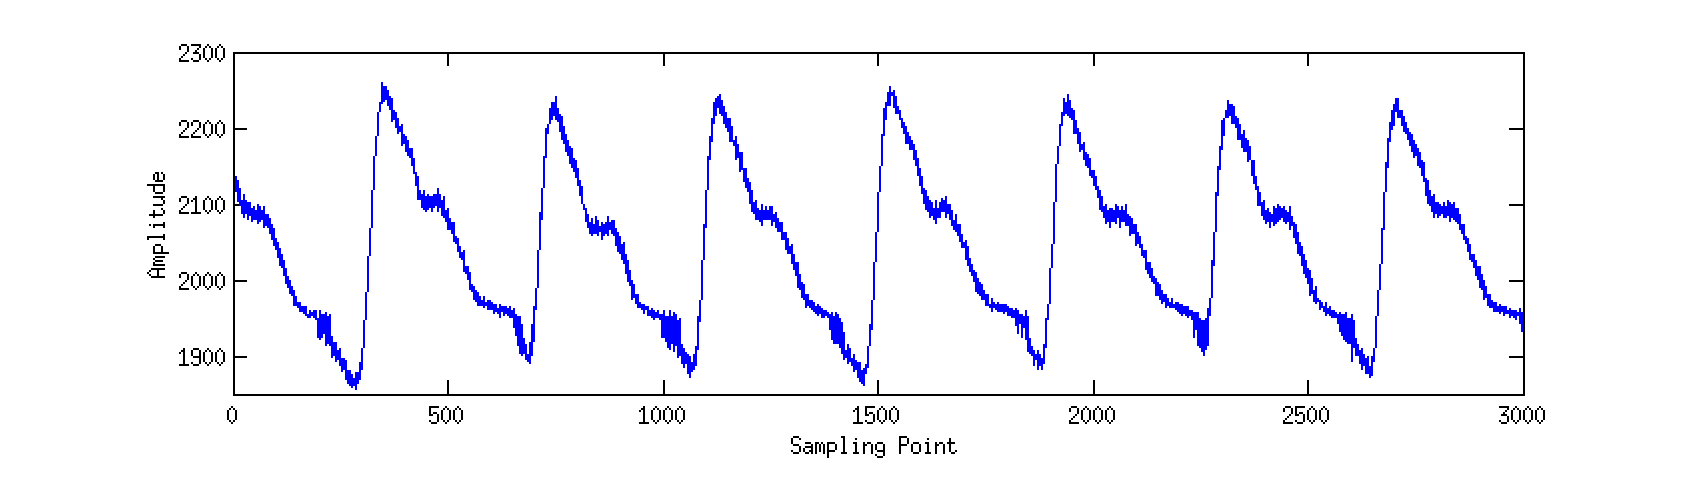
\includegraphics[width=0.9\textwidth]{adaptive}}\\
  \caption{The comparison of denoising effect with different thresholds}
  \label{fig:threshold}
\end{figure}

\subsection{Removal of electric power noise}
In carefully inspection to Figure~\ref{fig:soft}, it is found 
noise remaining in the tail of a period. So the frequency spectrum shown in
Figure~\ref{fig:powerfreqspec} shows the frequency distribution of noise.
The signal not only contains the electric power 50Hz noise, but also
noises higher than 50Hz from the internal system. 
The spike with frequency greater than 50Hz must be a burr noise since
the human pulse signal distributes below 15Hz.~\cite{wei1985frequency}
Hence, it is justified to remove all the noises upper than 50Hz.
So a low-pass linear filter is designed to filter them. 

Digital filters are typically considered in two categories: infinite impulse
response (IIR) and finite impulse response (FIR). FIR has two useful
properties which make it preferable to an IIR filter in this
experiment: inherent stability and linear phase. Linear phase implies an
important attribute because the pulse signal is a phase-sensitive
application. Although the disadvantage of FIR filters is that considerably more
computation power in a general purpose processor is required compared
to an IIR filter with similar sharpness or selectivity, properly
designed coefficients make FIR filters approximately as efficient as
IIR for many applications. 

The FIR filter is designed as these arguments: 
\begin{table}
    \centering
    \begin{tabular}{cc}
        Response type & Lowpass \\ \hline
        Design method & Kaiser Window \\ \hline
        Filter order & Minimum \\ \hline
        Frequency Specifications & $F_pass=48Hz, F_stop=50Hz$ \\ \hline
        Magnitude Specifications & $A_pass=1db, A_stop=80db$ \\\hline
    \end{tabular}
    \caption{The filter specifications}
    \label{tab:filter}
\end{table}
The magnitude response of the FIR filter under these arguments is
shown in Figure~\ref{fig:magnitutde}. By convolution filtering, the
noise with frequency higher than 50Hz is highly depressed.
Figure~\ref{fig:afterpower} gives the final pulse signal denoised. 
\begin{figure}[htpb]
    \begin{center}
        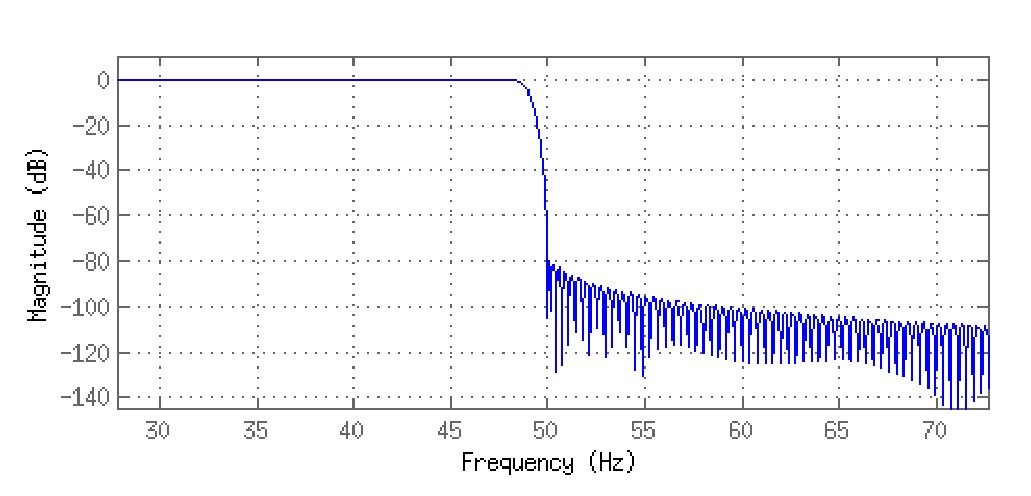
\includegraphics[width=0.7\textwidth]{filter}
    \end{center}
    \caption{Magnitude response of FIR filter}
    \label{fig:magnitutde}
\end{figure}

\begin{figure}
    \centering
    \subfloat[Pulse wave with power electric
    noise]{\label{fig:powernoise}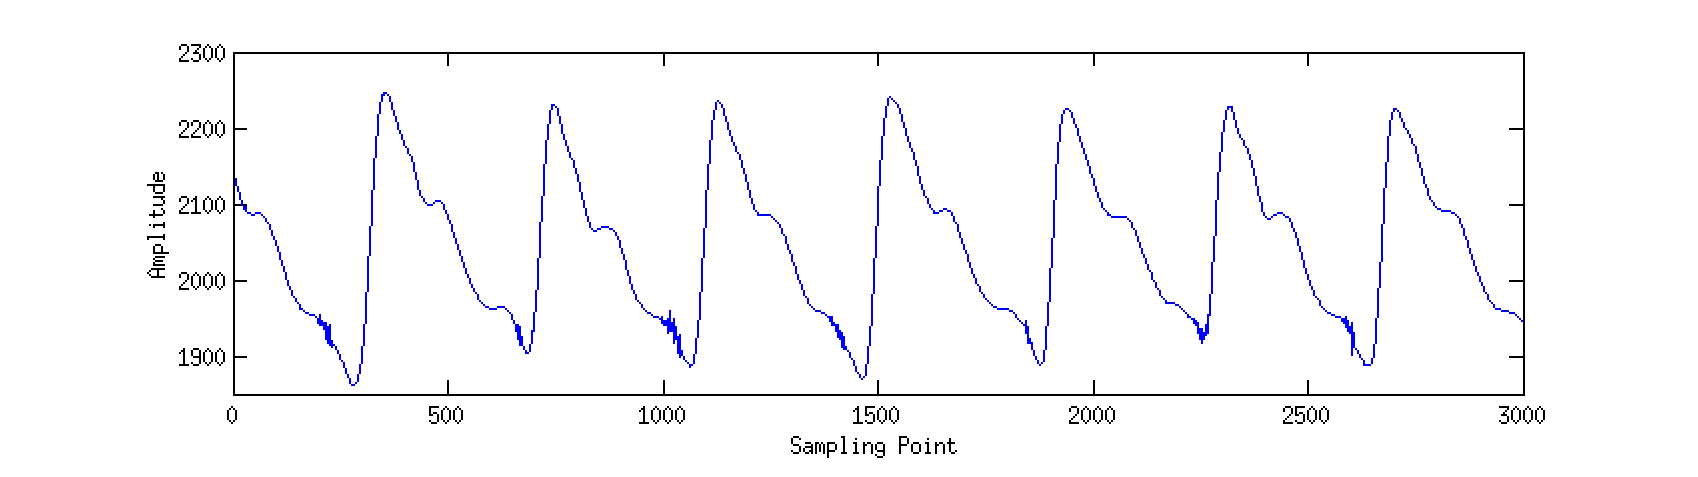
\includegraphics[width=0.7\textwidth]{soft}}\\
    \subfloat[The frequency
    spectrum]{\label{fig:powerfreqspec}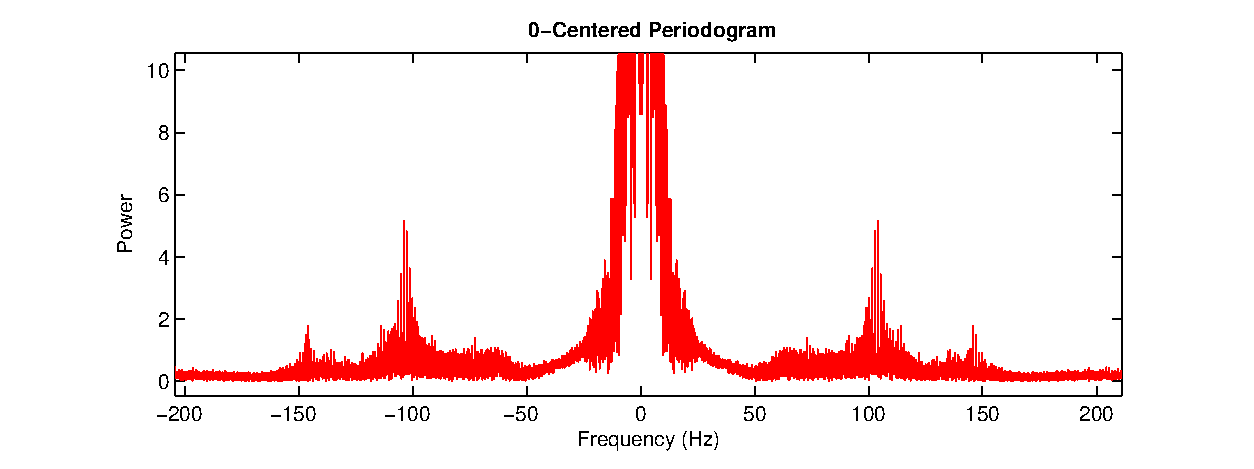
\includegraphics[width=0.7\textwidth]{50hz}}
    \caption{The pulse waveform before power noise removal}
    \label{fig:beforepower}
\end{figure}
\begin{figure}
    \centering
    \subfloat[Pulse wave after power electric noise
    removal]{\label{fig:nopowernoise}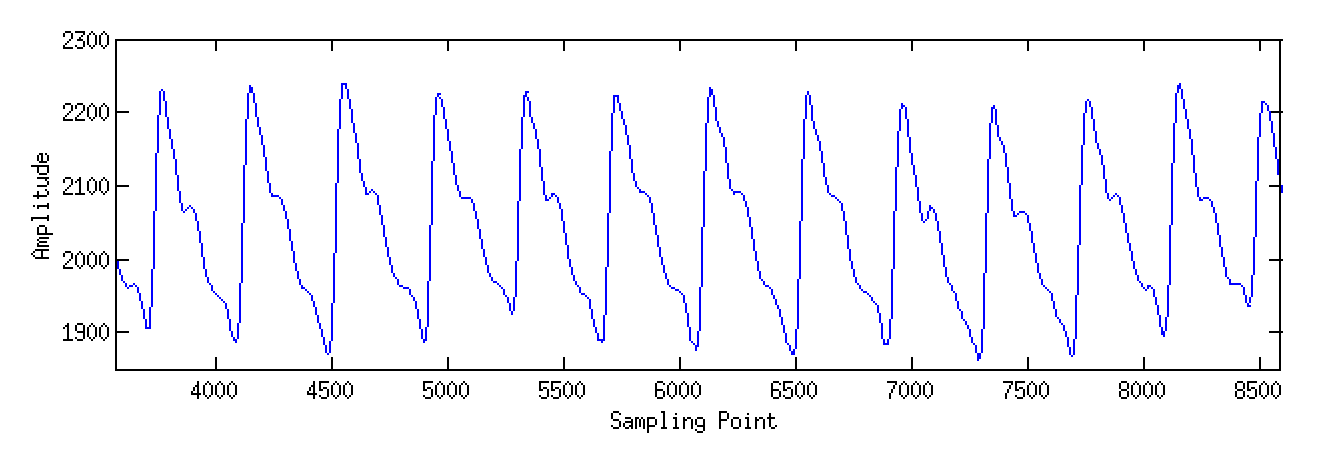
\includegraphics[width=0.7\textwidth]{after50Hz}}\\
    \subfloat[The frequency
    spectrum]{\label{fig:nopowerfreqspec}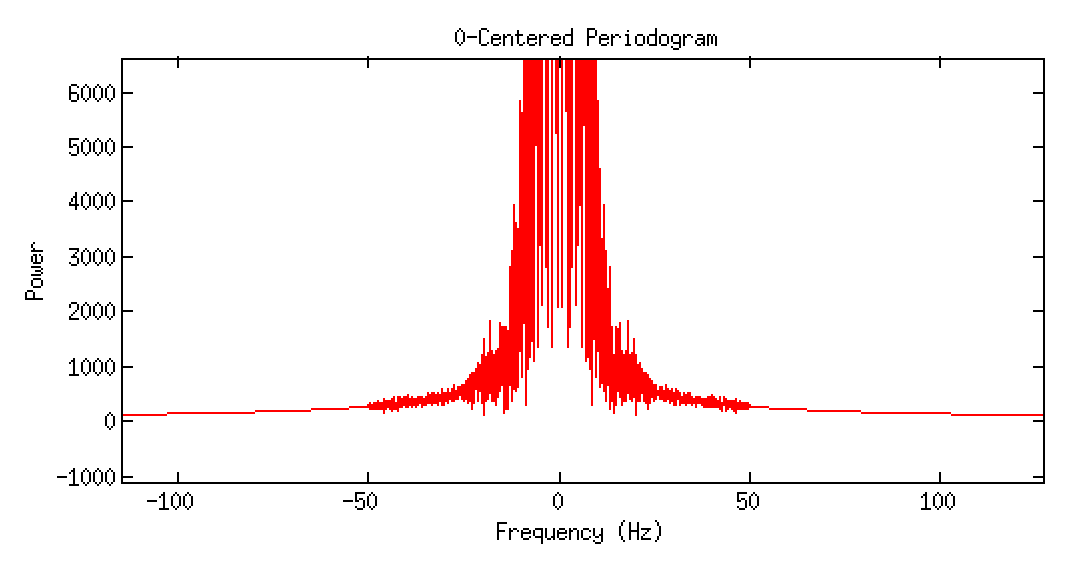
\includegraphics[width=0.7\textwidth]{freqspecafter}}
    \caption{The pulse waveform after power noise removal}
    \label{fig:afterpower}
\end{figure}

\section{Removal of pulse waveform baseline wander}
Although the collecting system the paper uses is linear-bandwidth
within [0.05Hz, 100Hz], the pulse waveform is yet interference by the
breathing and body movement during pulse capture. Otherwise, the pulse
signal of a healthy person will stay on a horizontal line, i.e. each
starting point of a pulse cycle lies on this horizontal line. See Figure~\ref{fig:baselinedrift}. As
similar to electrocardiogram (ECG) signal, the line is also called
\emph{baseline} in this paper. The baseline will bring waveform
distortion to feature extraction so as to affect the succeeding
analysis.~\cite{li1999study,allen2000variability} 
\begin{figure}[htbp]
    \begin{center}
        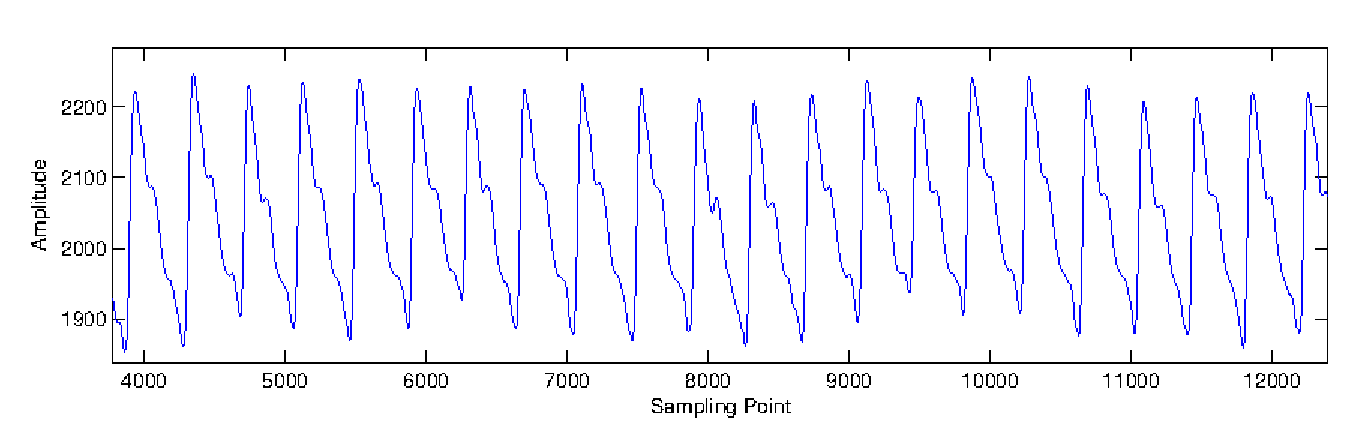
\includegraphics[width=0.8\textwidth]{baselinedrift}
    \end{center}
    \caption{The pulse wave with baseline drift}
    \label{fig:baselinedrift}
\end{figure}

The baseline wander issue has existed in physiological signal (e.g.
ECG) in a long time and many methods have been put forward in previous
work. These methods involves ensemble average, polynomial interpolation,
zero-phase filtering, morphological filtering, time-varying filtering,
adaptive filtering, wavelet-based filtering etc. All of them have
their specific applicable conditions. With the improvement of pulse
collecting system and the carefulness in actual mechanical process,
the quality of most pulse waveforms are remarkable with less severity
of baseline wander. Cubic spline interpolation is a simple but
effective approach to estimate the hidden baseline. Therefore, the
paper adopts it to remove baseline wander. 

\subsection{Starting point detecting technique}
\label{sec:startpoint}

Before beginning with the cubic spline interpolation approach, we
should detect where the starting point of each cycle is. To avoid
controversy, the \emph{starting point} in the paper prescribes the
nadir in the ascending limb. The paper employs a concept of
\emph{sliding window}. In detail, because the sampling frequency is
500Hz while the wrist pulse frequency lies in between 48Hz and 100Hz
(participants are required to calm down before collection), there must
exist at least a pulse cycle in every 500 points. The paper uses a
500 points sized window to find peaks in the whole pulse waveform. A
schematic diagram as Figure~\ref{fig:slidingwindow} can help understand. 
\begin{figure}[htpb]
    \begin{center}
        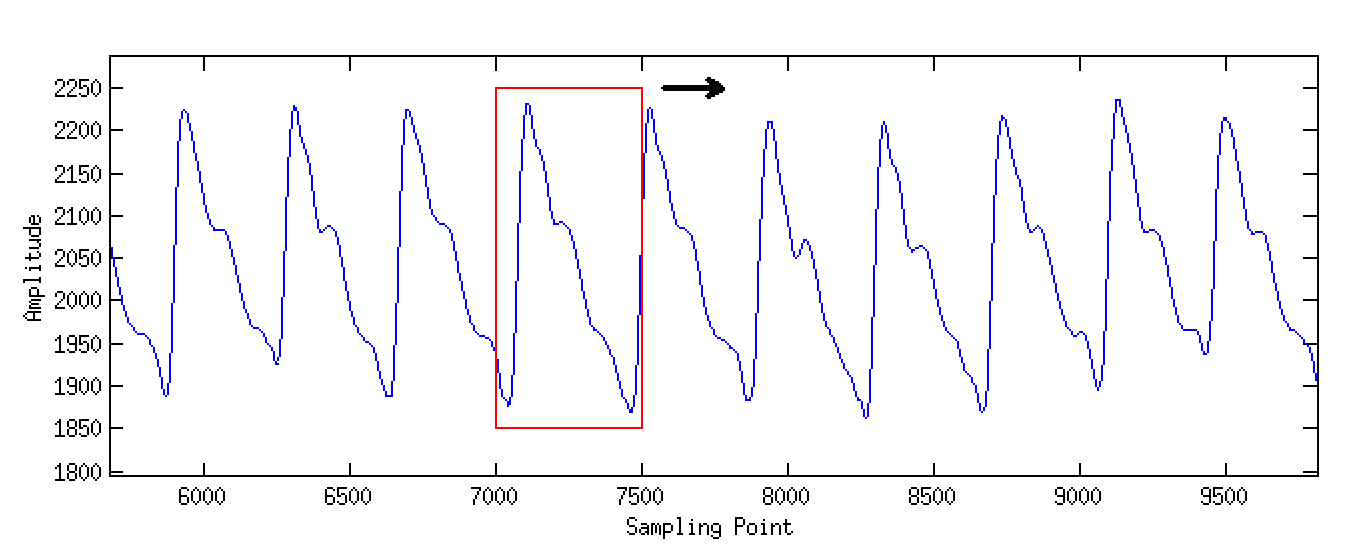
\includegraphics[width=0.7\textwidth]{slidingwindow}
    \end{center}
    \caption{The sliding window for peak detecting}
    \label{fig:slidingwindow}
\end{figure}

The peak detecting algorithm is described as follows:

\begin{algorithmic}
    \REQUIRE The denoised pulse waveform
    \ENSURE The peaks detected
    \STATE set window size as 500 points
    \FOR {each point $i$ from left to right}
        \STATE the window is the nearest 500 points centered on $i$
        \STATE find the maximum point in the window 
        \IF {the maximum point is current point $i$}
            \STATE mark $i$ as a peak
        \ENDIF
    \ENDFOR
\end{algorithmic}

Then, it is easy to get the starting points just by detecting the peaks of
up-down reversal pulse waveform using the algorithm above. The
practice on around 500 samples shows the robustness and accuracy of
this algorithm. See Figure~\ref{fig:startingpoint}.
\begin{figure}[htpb]
    \begin{center}
        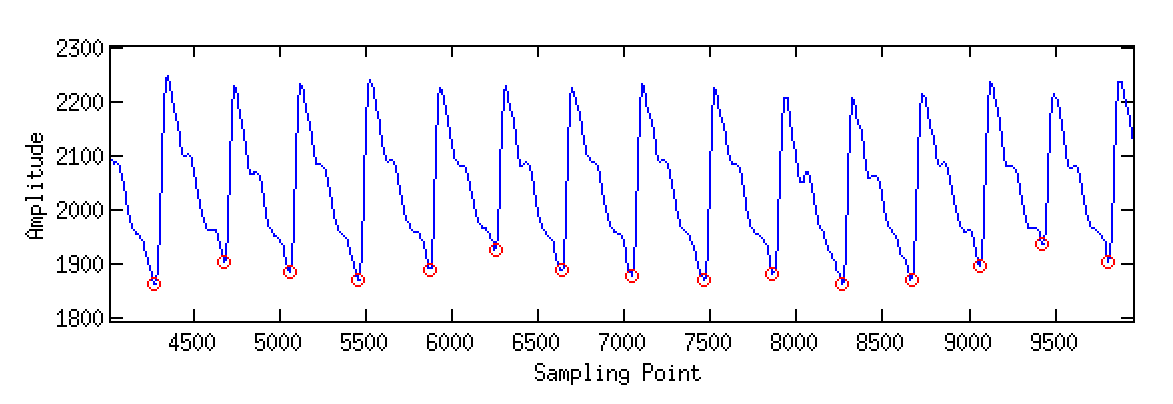
\includegraphics[width=0.7\textwidth]{startingpoint}
    \end{center}
    \caption{Starting points detected}
    \label{fig:startingpoint}
\end{figure}

\subsection{Cubic spline interpolation}
The baseline wander the breathing or body movement creates is
nonlinear and smooth, so the cubic spline interpolation could predict
the wandered baseline well. Estimation is actually a process of
function approximation. Spline interpolation is such an approximation
method to predict the major distribution from minor samples. Spline
interpolation is preferred over polynomial interpolation because the
interpolation error can be made small even when using low degree
polynomials for the spline. Spline interpolation avoids the problem of
Runge's phenomenon which occurs when interpolating between equidistant
points with high degree polynomials. 

Spline interpolation theory origins from the elastic ruler problem.
The mathematical model is described as this: The definition domain
$[a, b]$ is divided by a number of $n+1$ predefined points (the
``knots'') $(x_i, y_i)$ into small intervals $[x_i, x_{i+1}$, in
mathematical form of
$a=x_1<=\ldots<x_l=b$; The mission is to find a $n$ th-order spline
function $S(x)$ to piecewise estimate the objective function. A
piecewise cubic spline function $S(x)$ can be denoted as:
\begin{equation}
    S(x)=\sum_{k=0}^{3} a_k x^k + \sum_{i=1}{L} b_i
    (x-x_i)_{+}^{3} \quad for k=0,1,2,3; i=1,\ldots,L 
    \label{equ:cubic}
\end{equation}
\begin{equation}
    (x-x_i)_{+}^{3} = \left\{
    \begin{array}{ll}
        (x-x_i)^3, & (x \geq x_i)\\
        0, & (x<x_i)\\
    \end{array} \right.
    \label{equ:cubic2}
\end{equation}
where $a_k$ and $b_i$ denotes the polynomial coefficients and $L$
denotes the number of knots. From Equation~\ref{equ:cubic}, the
second-order differential of spline function $S(x)$ is 
\begin{equation}
    S''(x) = 2! \cdot a_2 + 3! \cdot a_3 \cdot x + 3! \cdot
    \sum_{i=1}^{L} \cdot (x-x_i)_{+}
    \label{equ:cubic3}
\end{equation}
The Equation~\ref{equ:cubic3} demonstrates that the second-order
differential in knot $(x_i, y_i)$ is continuous. Since the wandered baseline
is a continuously differentiable function, it implies that the
second-order differential of baseline is also continuous. The cubic
spline data interpolation can approach wandered baseline well. 
The Figure\ref{fig:estbaseline} and Figure~\ref{fig:baselined} respectively shows the wandered
baseline estimated and the pulse waveform after removal of baseline wander.
\begin{figure}[htpb]
    \begin{center}
        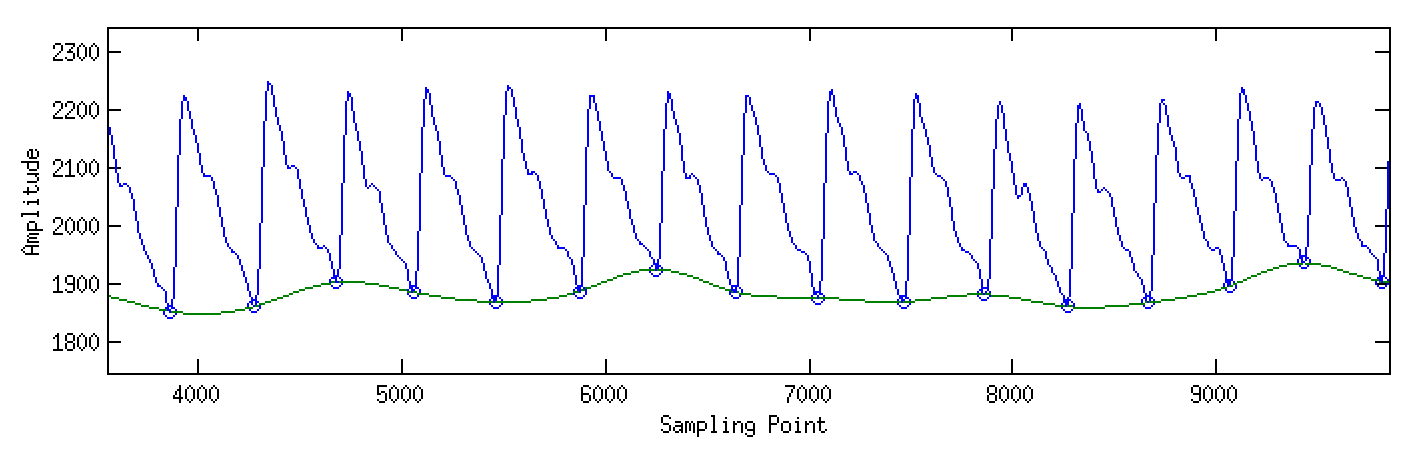
\includegraphics[width=0.7\textwidth]{cubic}
    \end{center}
    \caption{The estimated baseline wander using cubic spline interpolation}
    \label{fig:estbaseline}
\end{figure}
\begin{figure}[htpb]
    \begin{center}
        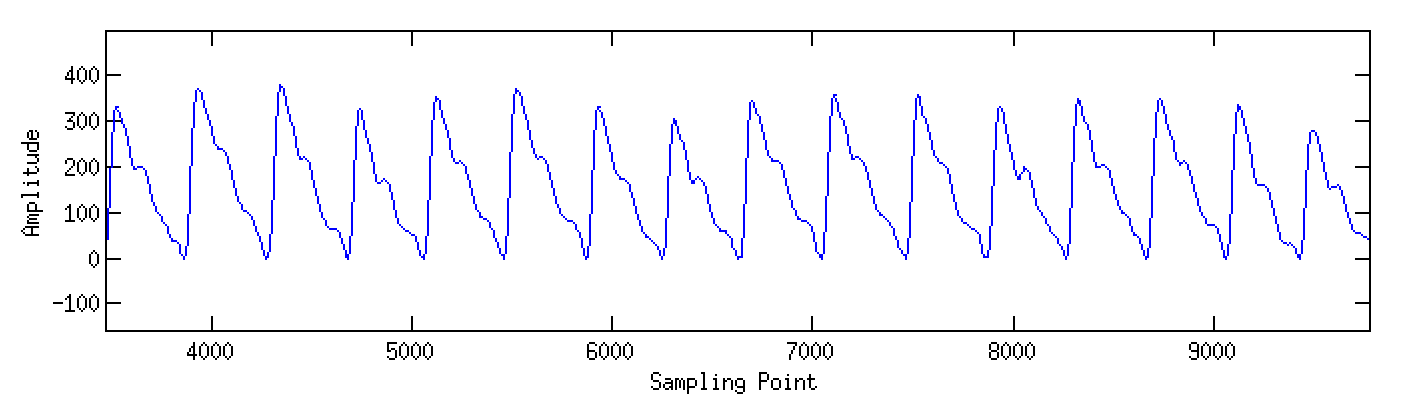
\includegraphics[width=0.7\textwidth]{baselined}
    \end{center}
    \caption{The pulse waveform after removal of baseline wander}
    \label{fig:baselined}
\end{figure}

\section{Period segmentation of pulse waveform}
The pulse image is a quasi-periodic waveforms, in which a period of
waveform records most information about wrist pulse. Beginning
with a single period pulse analysis is an effective way to understand 
in-depth meaning of pulse. The data processing in succeeding chapters
of the paper is built on a single period pulse waveform. So the
foregoing preprocessed pulse must split into single periods. 

The period segmentation, as implied by the name, is to find the starting
point and the end point. The end point is also the starting point of
next period. So only starting points are necessary to find out.
Remember the Section~\ref{sec:startpoint} introduced an algorithm
detecting the starting points. The task of period segmentation comes
much easier with the algorithm. Find two adjacent starting points
randomly and extract the period between these two points.

\section{Normalization of pulse waveform }
Because of the diversity of collecting environment and the individual
differences, the pulse may differ remarkably in amplitude. To treat them
as equal, the paper will take measures to normalize the preprocessed single
period pulse wave. Let $x$ denote a small segment signal and 
$y$ denote the normalized signal,  the
linear normalization formula is given as:
\begin{equation}
    y = \frac{x-max(x)}{max(x)-min(x)}
    \label{equ:normalize}
\end{equation}
where $max,min$ are operations to extract the maximum and the minimum,
respectively. A typical single period signal after denoising
, baseline removal and normalization pre-processing is displayed as
Figure~\ref{fig:normalize}.
\begin{figure}[htpb]
    \begin{center}
        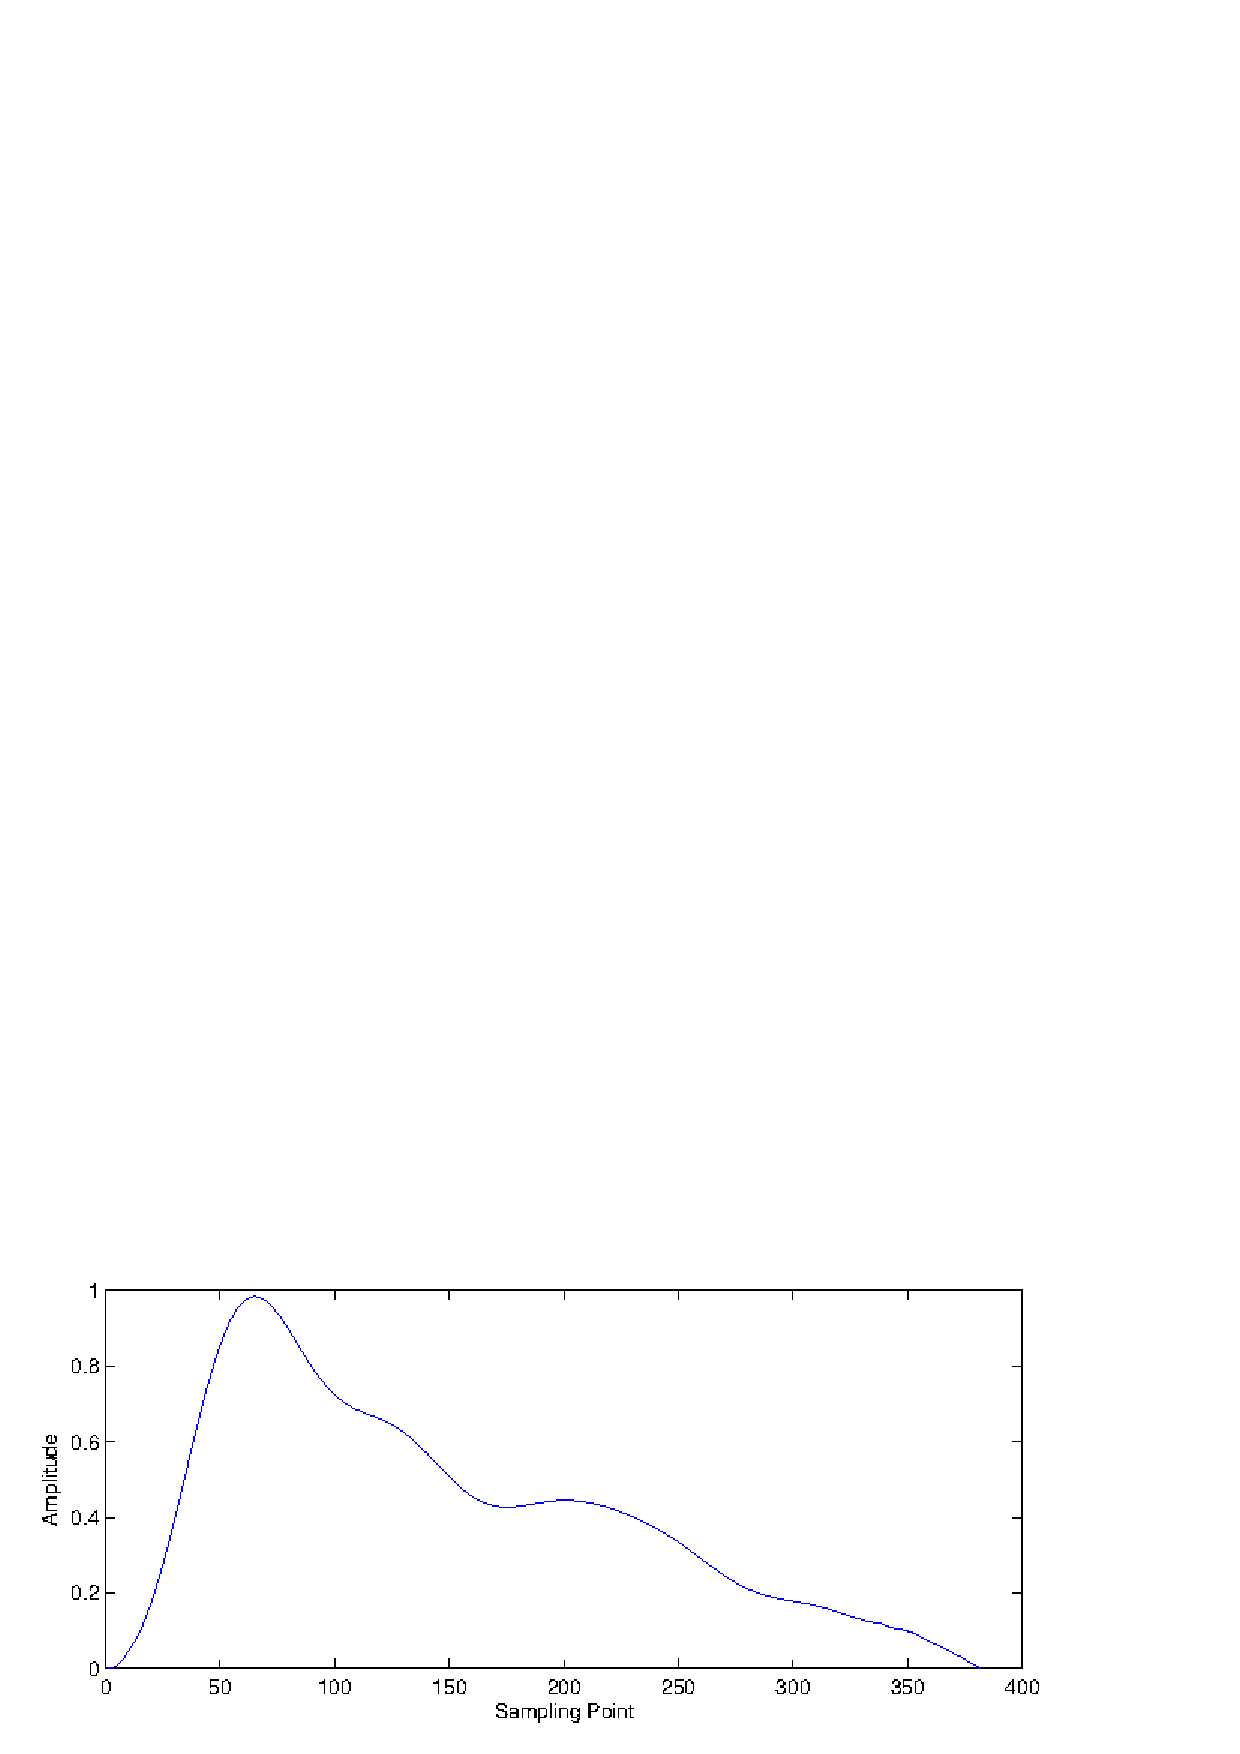
\includegraphics[width=0.7\textwidth]{normalized}
    \end{center}
    \caption{The normalized pulse signal}
    \label{fig:normalize}
\end{figure}


\section{Summary}
The chapter pre-processes the original pulse signal as needed,
including burring, baseline wander removal, segmentation and
normalization. First, the paper adopts \emph{sym8} wavelet tool and
digital linear filter to remove the high frequency noise. Second,
the simple but effective cubic spline interpolation method is applied to solve the baseline
drift issue. Finally, the optimized pulse waveform is separated into
independent periods and normalized. The single period pulse waveform
is the real input for the following chapters. 


\chapter[Pulse feature extraction]{\uppercase{Pulse feature extraction}}
\label{chap:four}

Different from the traditional pulse diagnosis, the digitized wrist
pulse in the paper is an objectified, precisely quantified,
standardized and automated pulse signal. As an important issue in
pattern classification field, feature extraction directly affects the
design and performance of classifier. If the features extracted from
distinct classes sharply differ from one another, it is easy to design a
high discrimination classifier. Thus, Thus, how to extract features from the
sample effectively is a tremendous step in pulse patter
classification process. \todo{时域频域}

\section{Time-domain features}
\subsection{Time-domain features and its physiological significance}
A complete cycle of pulse waveform consists of an ascending limb and a
descending limb, shown as Figure~\ref{fig:waveform}. The ascending limb results from the systole activity:  
When systole occurs, the left ventricle ejects blood to the aorta in the sphygmic
period; The increase of blood pressure causes the elastic expansion
of aorta, that leads to the displacement of vascular wall. Likewise,
the descending limb occurs in the late systole period when the blood
ejection rate slows down; The pressure in the aorta decreases and then the
vascular wall shrinks. 
The minimum point as point 3
in the figure is called dicrotic notch. In physiological view, it
denotes a small downward deflection in the arterial pulse or pressure
contour immediately following the closure of the semilunar valves and
preceding the dicrotic wave, sometimes used as a marker for the end of
systole or the ejection period. The secondary peak in the figure is
called tidal wave while the third peak is called dicrotic wave. 
These peaks and troughs construct an entire pulse cycle. 
\begin{figure}[htbp]
    \begin{center}
        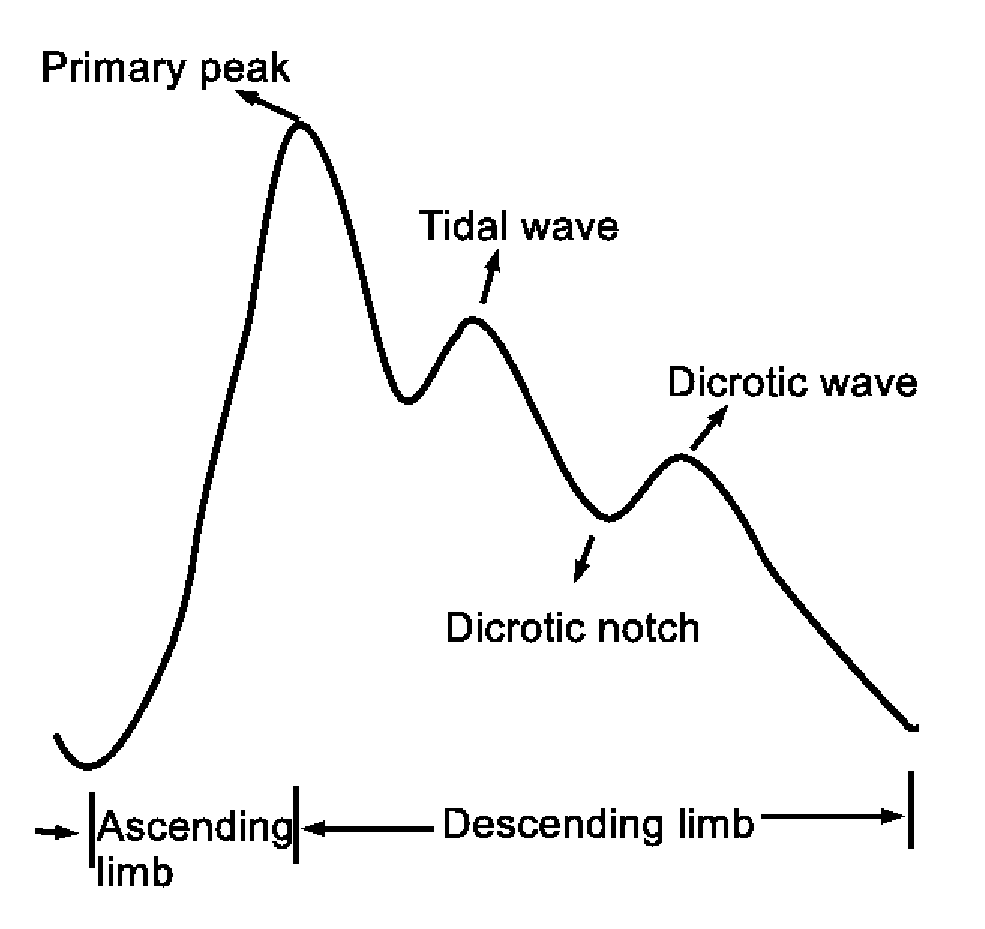
\includegraphics[width=0.4\textwidth]{pulsewaveform}
    \end{center}
    \caption{The basic structure of pulse waveform}
    \label{fig:waveform}
\end{figure}

The pulse image is the locus of vascular pulsation, so it has a
certain amount of significance. It integrates the information of 
vibration in cardiac ejection period and the pulse propagation along
vessels, which is reflected as the curve and inflection point in pulse
image. Some critical parameter illustrated in Figure~\ref{fig:timefeatures} and its
explanation could reveal the physiological meaning of pulse image.
\begin{figure}
    \centering
    \subfloat[shape
    features]{\label{fig:shape}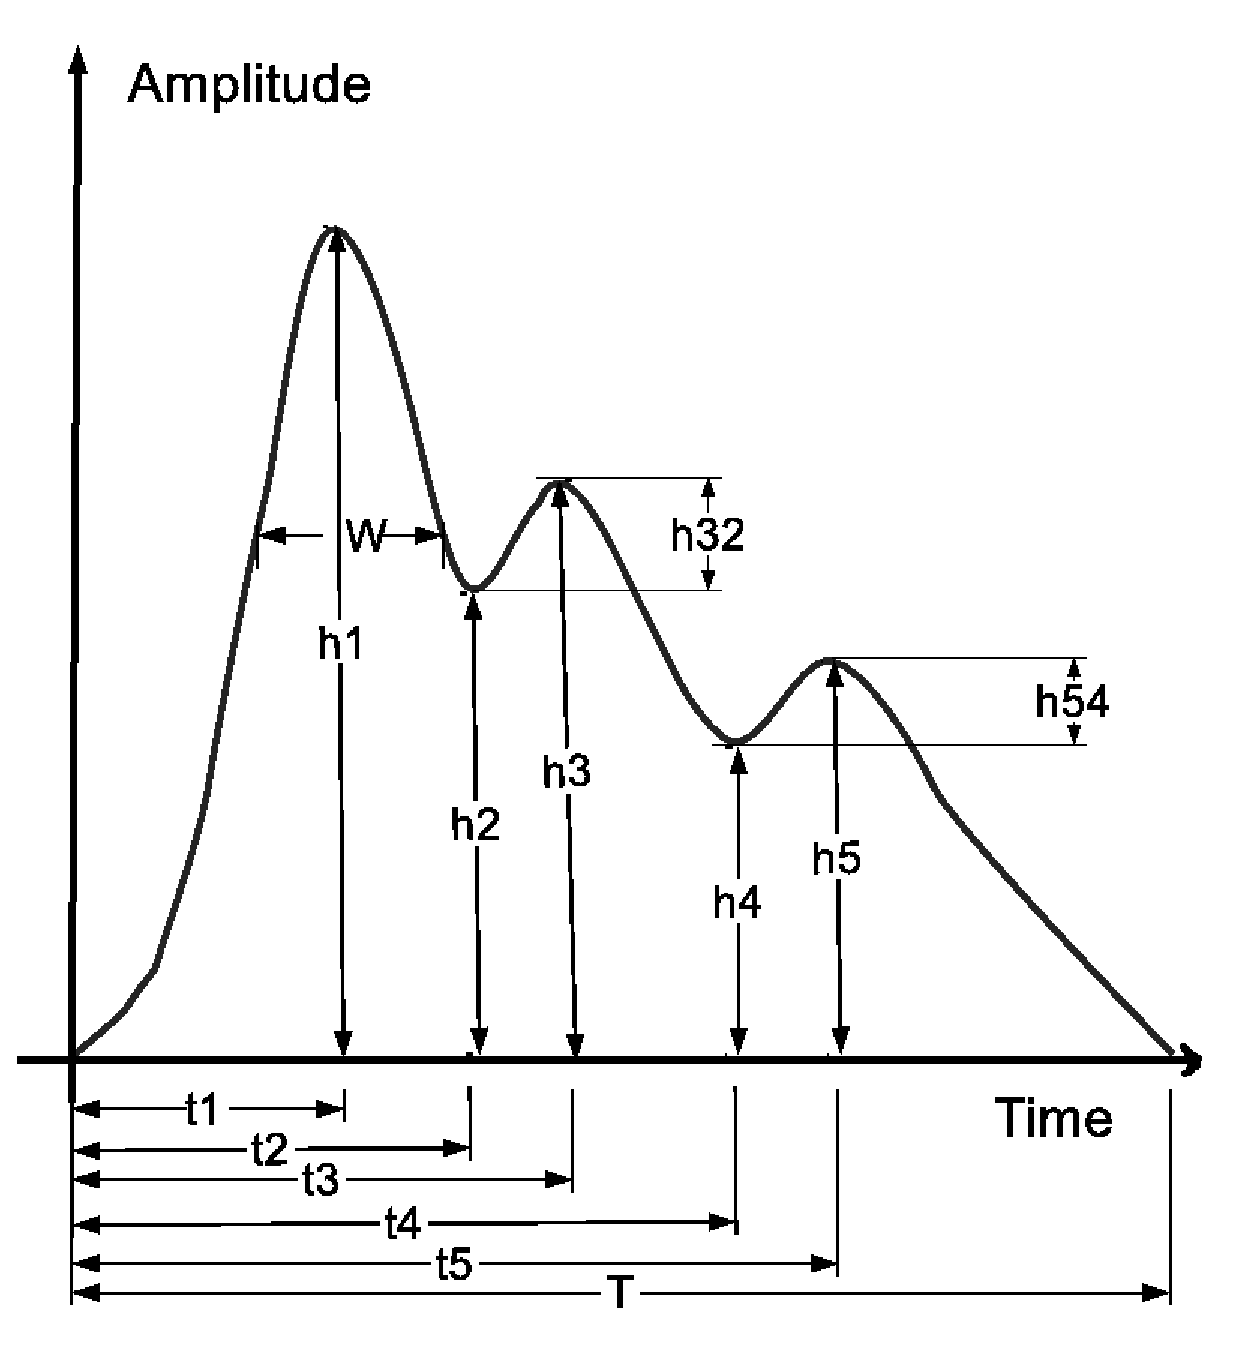
\includegraphics[width=0.3\textwidth]{shapefeatures}}
    \subfloat[area
    features]{\label{fig:area}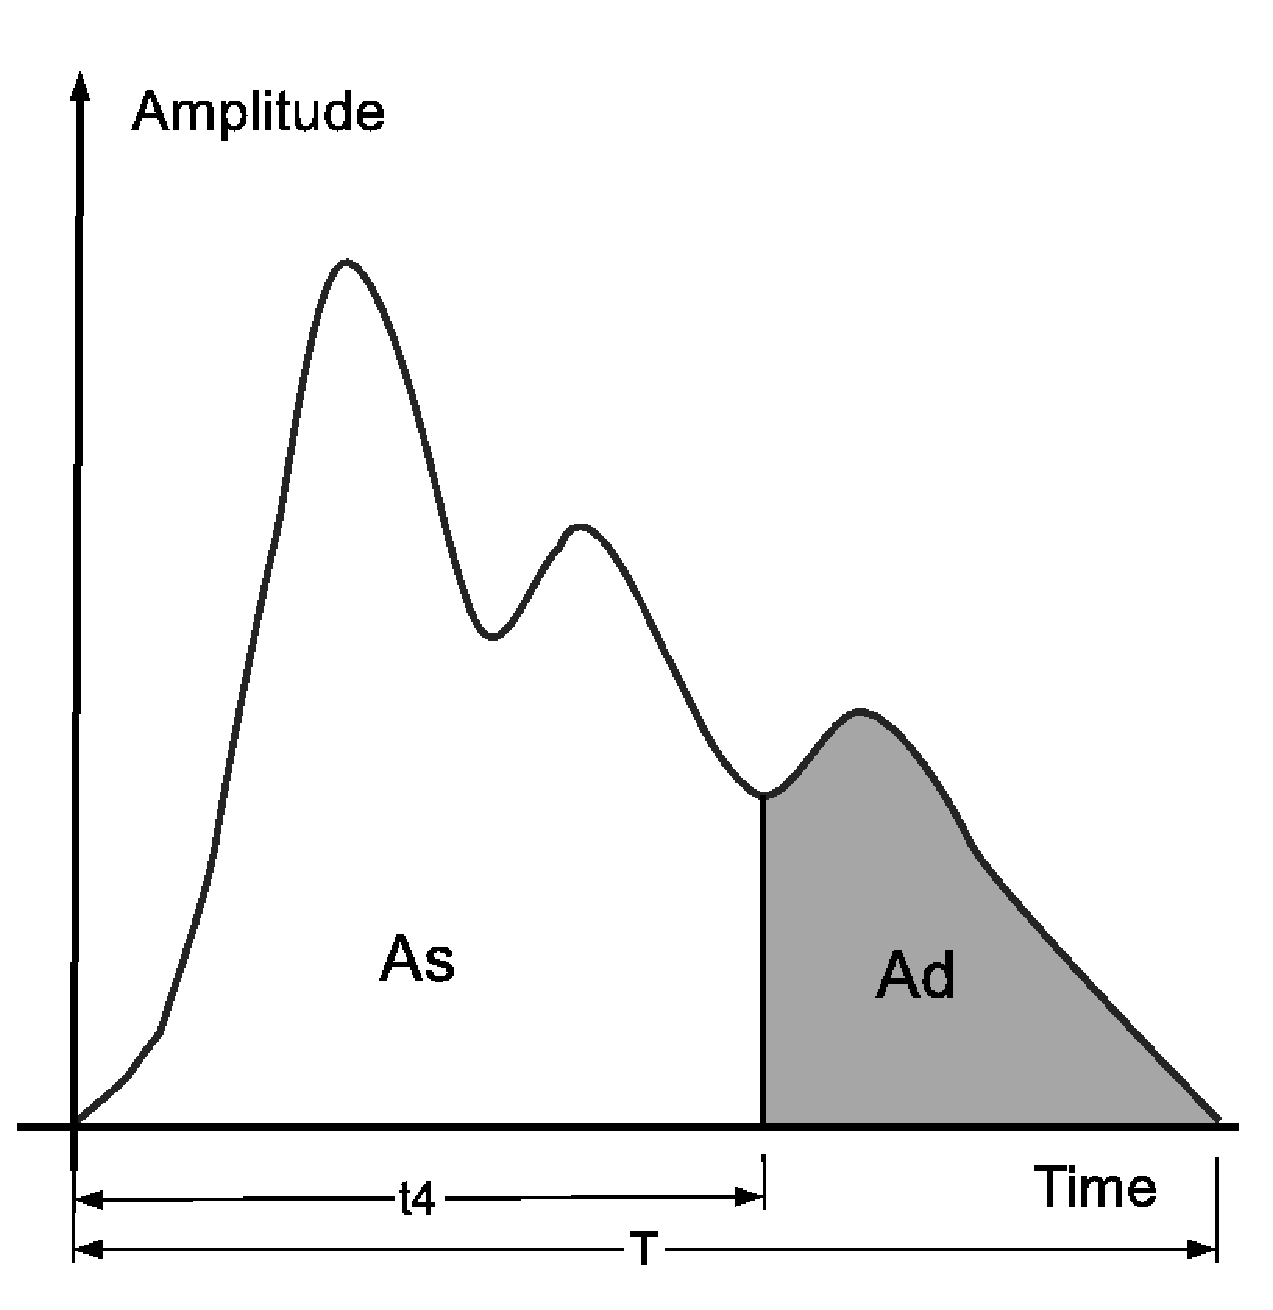
\includegraphics[width=0.3\textwidth]{areafeatures}}
    \caption{Time-domain features}
    \label{fig:timefeatures}
\end{figure}

These time-domain features represent special meanings as follows:
\begin{description}
    \item[h1:] The amplitude of primary wave. It is the height from
        the primary peak to x-axis (time base). The height reflects
        the sphygmic capacity of left ventricle and the arterial
        adaptability. Generally speaking, the stronger of the two
        capacity, the higher h1 is. Otherwise, the smaller h1 is. 
    \item[h2:] The amplitude of primary notch. It is the trough
        height between the primary wave and tidal wave.
    \item[h3:] The amplitude of tidal wave, i.e. the distance from the
        peak of tidal wave to x-axis. It reflects the arterial
        elasticity and peripheral resistance state. The amplitude h3
        would increase either if the arterial wall tension arises or
        if vascular sclerosis occurs or if the surrounding resistance
        arises. The elevation of tidal wave is often accompanied with
        the advance of time phase, which demonstrates a faster
        propagation rate of reflected wave in a state of high arterial
        tension and high resistance. 
    \item[h32:] The peak height of tidal wave. 
    \item[h4:] The amplitude of dicrotic notch, i.e. the distance
        between the trough of dicrotic notch to the x-axis, 
        corresponding to the diastolic pressure. It relates with arterial
        peripheral resistance and the aorta valve function. In
        general, h4 increases along with the rise of peripheral
        resistance. Otherwise, h4 decreases. 
    \item[h5:] The amplitude of dicrotic wave, i.e. the distance
        from the peak of dicrotic wave to the line across the trough
        of dicrotic notch, parallel to x-axis. The amplitude mainly
        reflects the aortic elasticity and aortic valve function. When
        the aortic adaptability diminishes or the aortic valve
        scleroses, h5 will eliminate correspondingly.  
    \item[h54] The peak height of dicrotic wave.
    \item[T] The time of a cycle, a.k.a. pulsation period,
        corresponding to a cardiac cycle of left ventricle. However,
        the pulse and ECG cardiac cycle will not be the same at the
        time of auricular fibrillation or extrasystole. 
    \item[t1] The time from start point of a cycle to the peak point,
        corresponding to rapid left ventricle ejection period. 
    \item[t2] The time from start point to the primary notch.
    \item[t3] The time from start point to the tidal wave peak point
    \item[t4] The time from start point of a cycle to dicrotic
        notch point, corresponding to the systole period of left
        ventricle. 
    \item[t5] The time from start point to the dicrotic wave peak
        point. 
    \item[W] The dominant peak width, where the junction height is
        defined as 2/3 of h1.
    \item[As] Area in systole period, related to the ejected blood volume. 
    \item[Ad] Area in diastole period.
    \item[PeakNum] the number of peaks. 
\end{description}

As can be seen from Figure~\ref{fig:keypoint}, the detection of key points A,
B, C, D, E, F is the critical step in time-domain features. Only if
these points are detected, can the calculation of the time-domain
relative features be launched. 
\begin{figure}[htpb]
    \begin{center}
        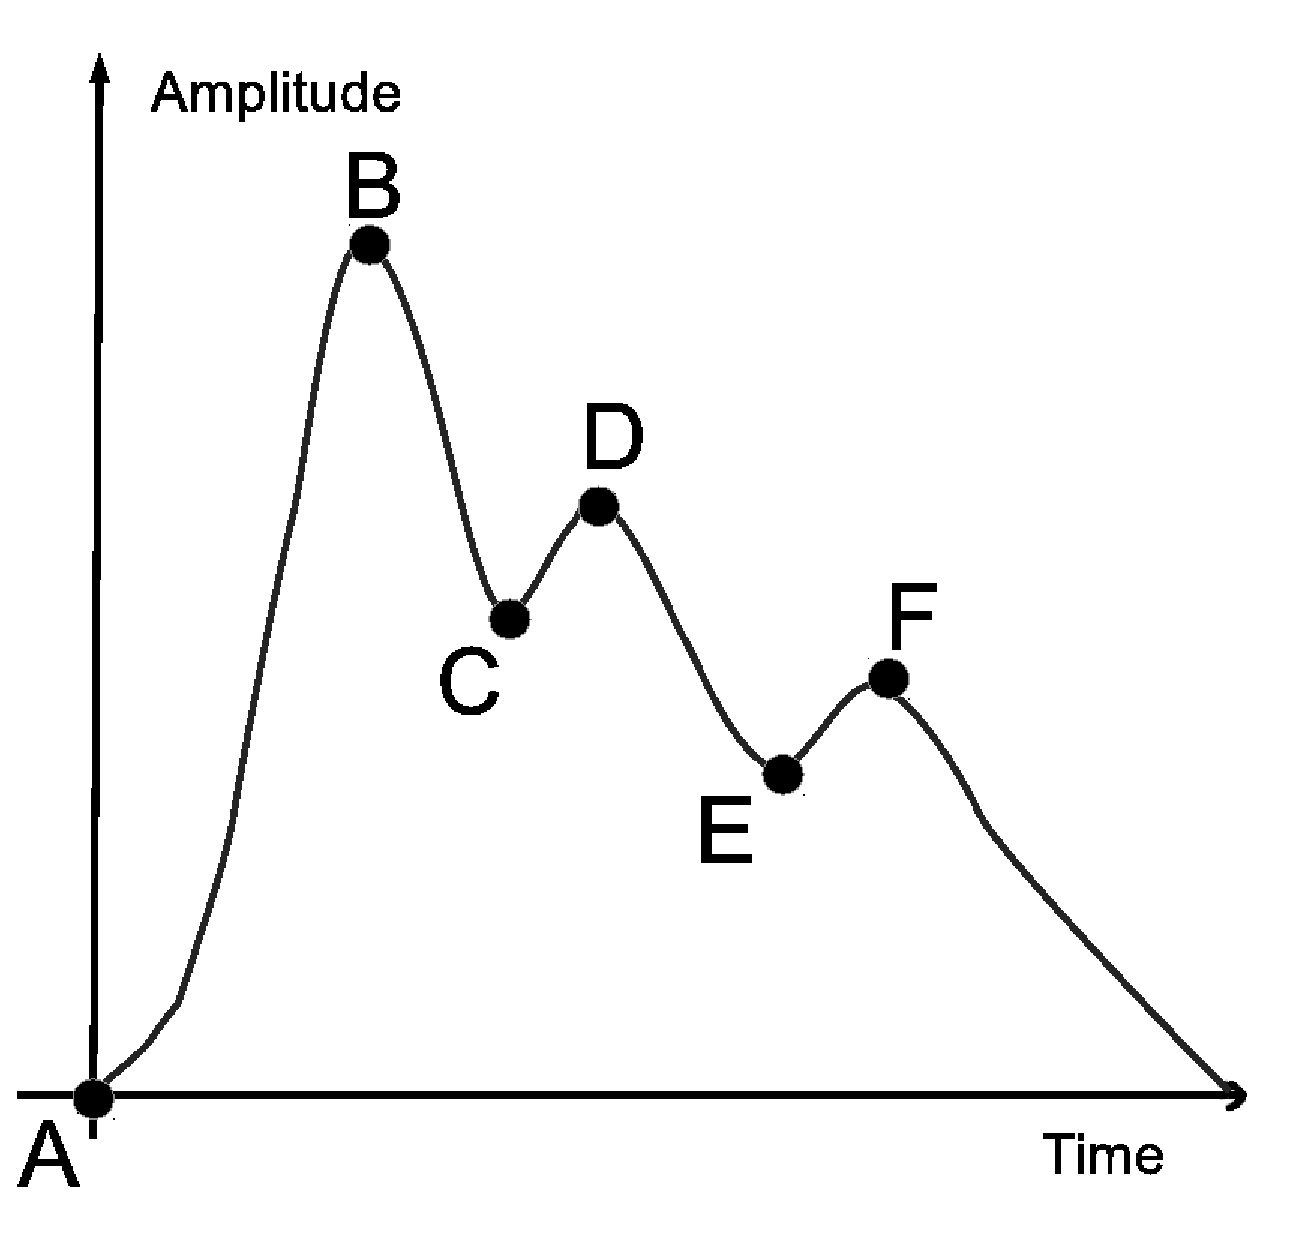
\includegraphics[width=0.4\textwidth]{keypoint}
    \end{center}
    \caption{The key points in a pulse cycle}
    \label{fig:keypoint}
\end{figure}
In fact, it can be seen that the
feature extraction is equivalent to the search of peak/trough points,
where the first derivative is zero. A derivative-based zero-cross
analysis is utilized for this purpose, and the peak search method are as follows:
\begin{enumerate}[(1)]
    \item Let the peak search range to be $0.85T$, which saves computing
        time. It is mainly because
        all peaks are located within the first 85\% of the waveform
        range after careful inspection. It is illustrated as the blue
        dotted line in Figure~\ref{fig:keypointsdetect}.
    \item Calculate the derivative of the signal, $d(t)$, as displayed
        in Figure~\ref{fig:firstderivative}. Since the pulse
        waveform is actually a sampled discrete signal, difference
        operation is applied in this case. There are many finite difference
        methods, e.g. forward difference $\Delta f(x)=f(x+1)-f(x)$,
        backward difference $\nabla f(x)=f(x)-f(x+1)$, central
        difference $\delta[f](x)=f(x+\frac{1}{2}h)-f(x-\frac{1}{2})$.
        The paper choose a eclectic approach between backward
        difference and forward difference. The form is given as:
        \begin{equation}
            x'_i=\left\{ 
            \begin{array}{ll}
                \frac{(x_i-x_{i-1})+(x_{i+1}-x_{i-1})/2}{2}, & i=2,\ldots,N-1\\
                x'_2, & i=1\\
                x'_N, & i=N-1\\
            \end{array} \right.
            \label{equ:1stdiff}
        \end{equation}
        \begin{equation}
            x''_i=\left\{ 
            \begin{array}{ll}
                \frac{(x'_i-x'_{i-1})+(x'_{i+1}-x'_{i-1})/2}{2}, &
                i=2,\ldots,N-1\\
                x''_2, & i=1\\
                x''_N, & i=N-1\\
            \end{array} \right.
            \label{equ:2nddiff}
        \end{equation}
        This eclectic derivative estimation method has advantages over
        the traditional method, which considers only two points, in
        robustness and generality. The method considers three points
        at meantime and is more accurate. Because this difference
        method makes no sense on the first point and the last point,
        let the derivative of second point and the one of penultimate
        point approximate to them, respectively.  
    \item Search the zero-cross points $d_i\;(i=1\,to\,5)$ in
        the derivative figure, and determine the revelent $h_i$ and
        $t_i$. 
    \item Search the first two points $P_1$ and $P_2$ whose amplitude equals to
        $2/3h_i$ within $[0,t_1]$ and $[t_1, t_2]$, respectively, and
        calculation the width $W=t(P_1)-t(P_2)$.
\end{enumerate}
\begin{figure}
    \centering
    \subfloat[The detected key
    points]{\label{fig:keypointsdetect}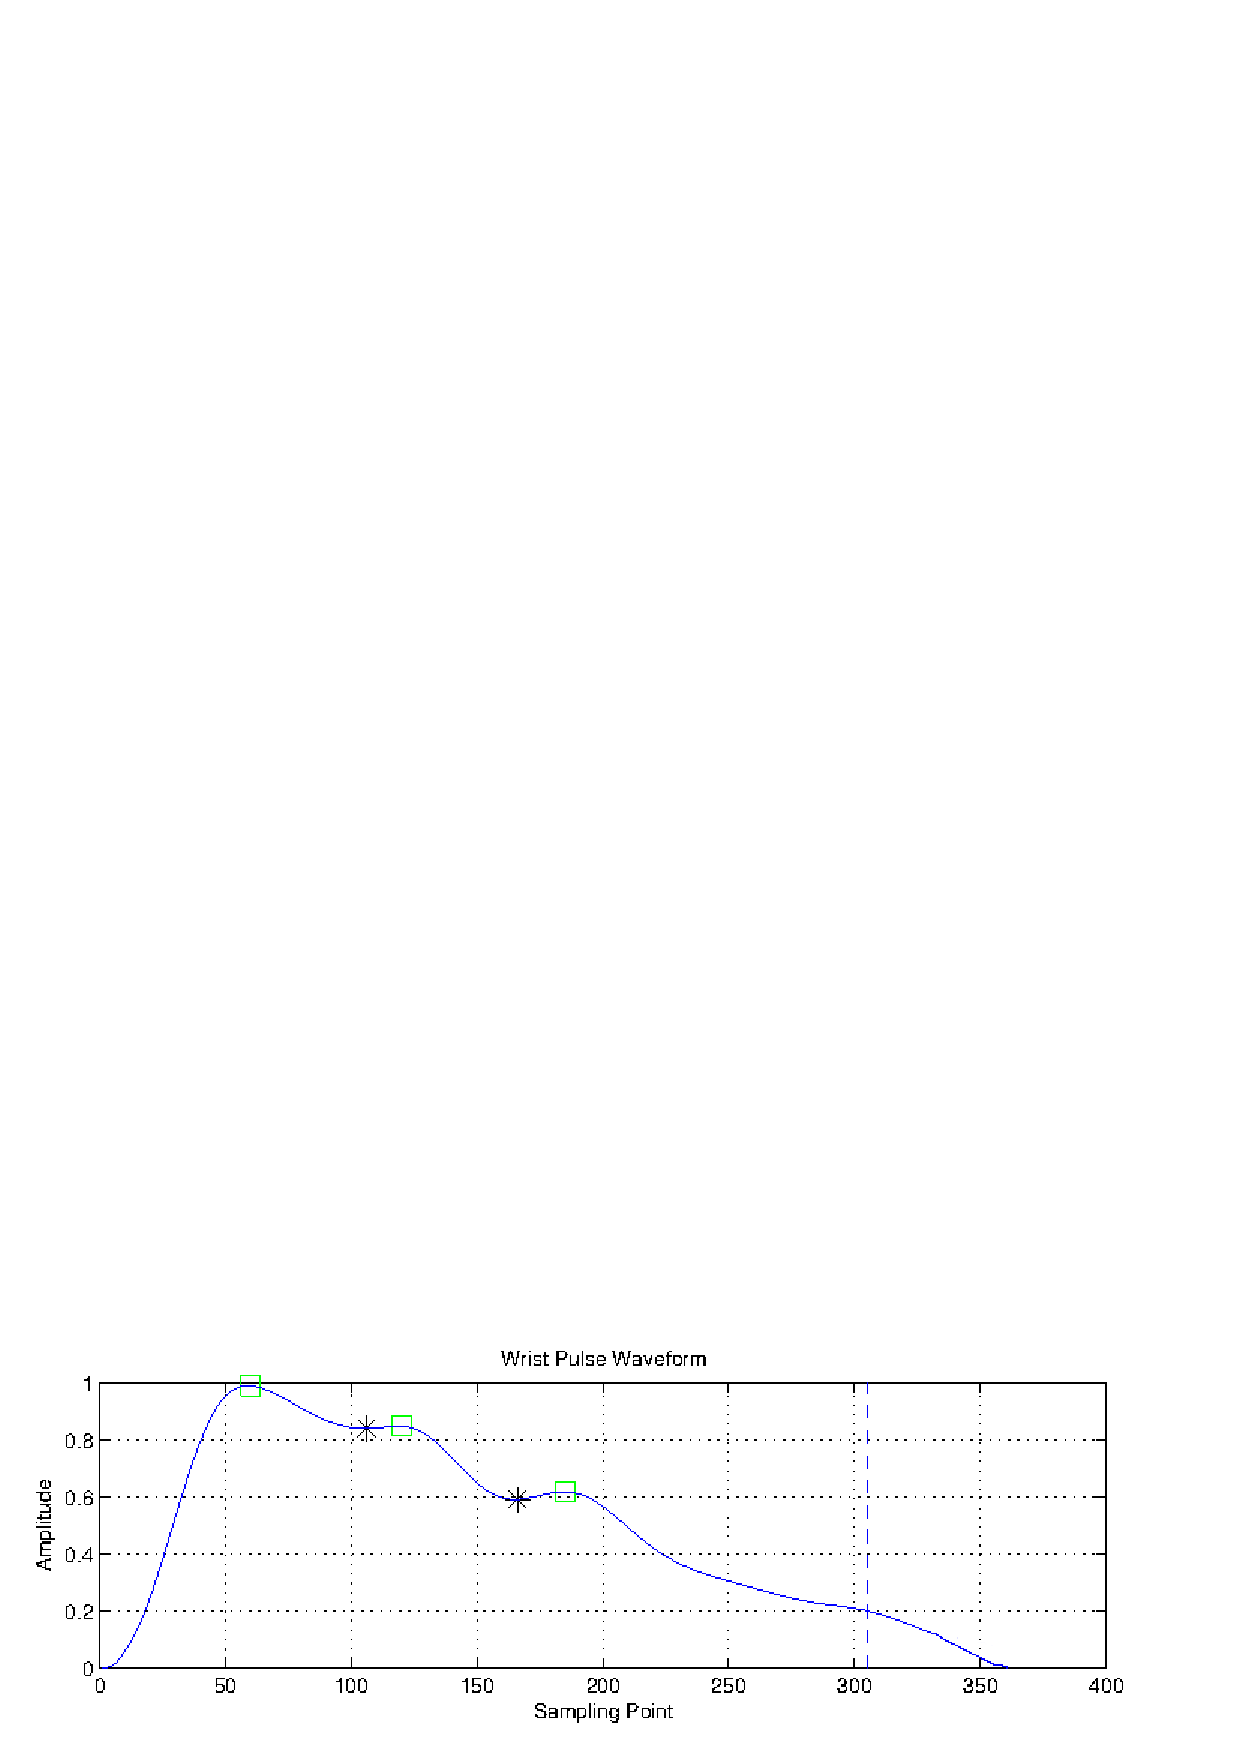
\includegraphics[width=0.6\textwidth]{keypointsdetected}}\\
    \subfloat[The first derivative of pulse
    waveform]{\label{fig:firstderivative}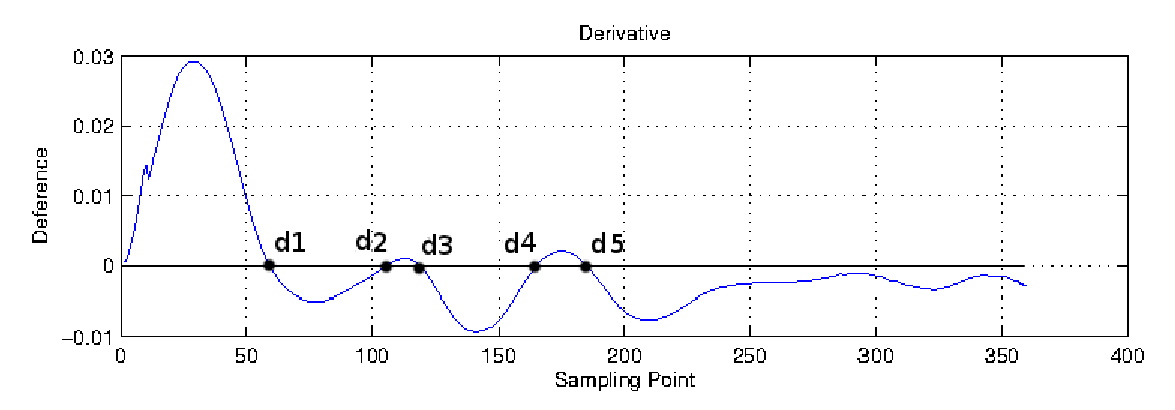
\includegraphics[width=0.6\textwidth]{firstderi}}
    \caption{The key points detected by the algorithm}
    \label{fig:keypointsgroup}
\end{figure}


Of course, these shape features may differ person by person. In
practice, for some pulse waveforms, the tidal wave may ``disappear'',
i.e. the tidal wave is so close to the primary peak that the height of
primary notch is still greater than the peak tidal wave. The
\emph{Xian Mai} is a typical case, shown in Figure~\ref{fig:xianmai}.
For such case, the zero-crossing points for $h_2$ and $h_3$ is missed.
To solve the issue, the paper introduces a \emph{tolerance} $\delta$ to find
the hidden pseudo trough and peak. An automated moving line
crossing point search is performed to get pseudo $h_2$ and $h_3$, which
equivalent to the search of points $d_1$ and $d_2$. The algorithm is
as follows:
\begin{enumerate}[(1)]
    \item Let the search range from $d_1$ to $d_4$;
    \item Find the maximum point within the range in the first-order
        deference, i.e. find all the
        zero-cross from positive to negative in the second-order
        deference (Figure~\ref{fig:2nddiff}). The point $d_{2(3)}$ in
        the first-order difference corresponds to its derivative point
        $dd_23$ in the second-order difference. 
    \item Check the validity of $d_{2(3)}$. 
        \begin{enumerate}[a)]
            \item If the maximum is upper than the dotted line
                $-\delta$ in the first-order difference
                (Figure~\ref{fig:1stdiff}, i.e. $d_{2(3)}<0 \; \& \;
                d_{2(3)} > -\delta$, then the sampling point $d_{2(3)}$ is a valid
                hidden peak of tidal wave.
            \item If the maximum is lower than the dotted line
                $-\delta$ in the first-order difference, i.e.
                $d_{2(3)}<-delta$, then the sampling point
                $d_{2(3)}$ is ignored.
        \end{enumerate}
\end{enumerate}

\begin{figure}[htbp]
    \begin{center}
        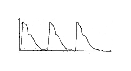
\includegraphics[width=0.5\textwidth]{xianmai}
    \end{center}
    \caption{Xian Mai: hidden tidal wave}
    \label{fig:xianmai}
\end{figure}

\begin{figure}
    \centering
    \subfloat[The pulse waveform of hidden tidal
    wave]{\label{fig:hiddenpulse}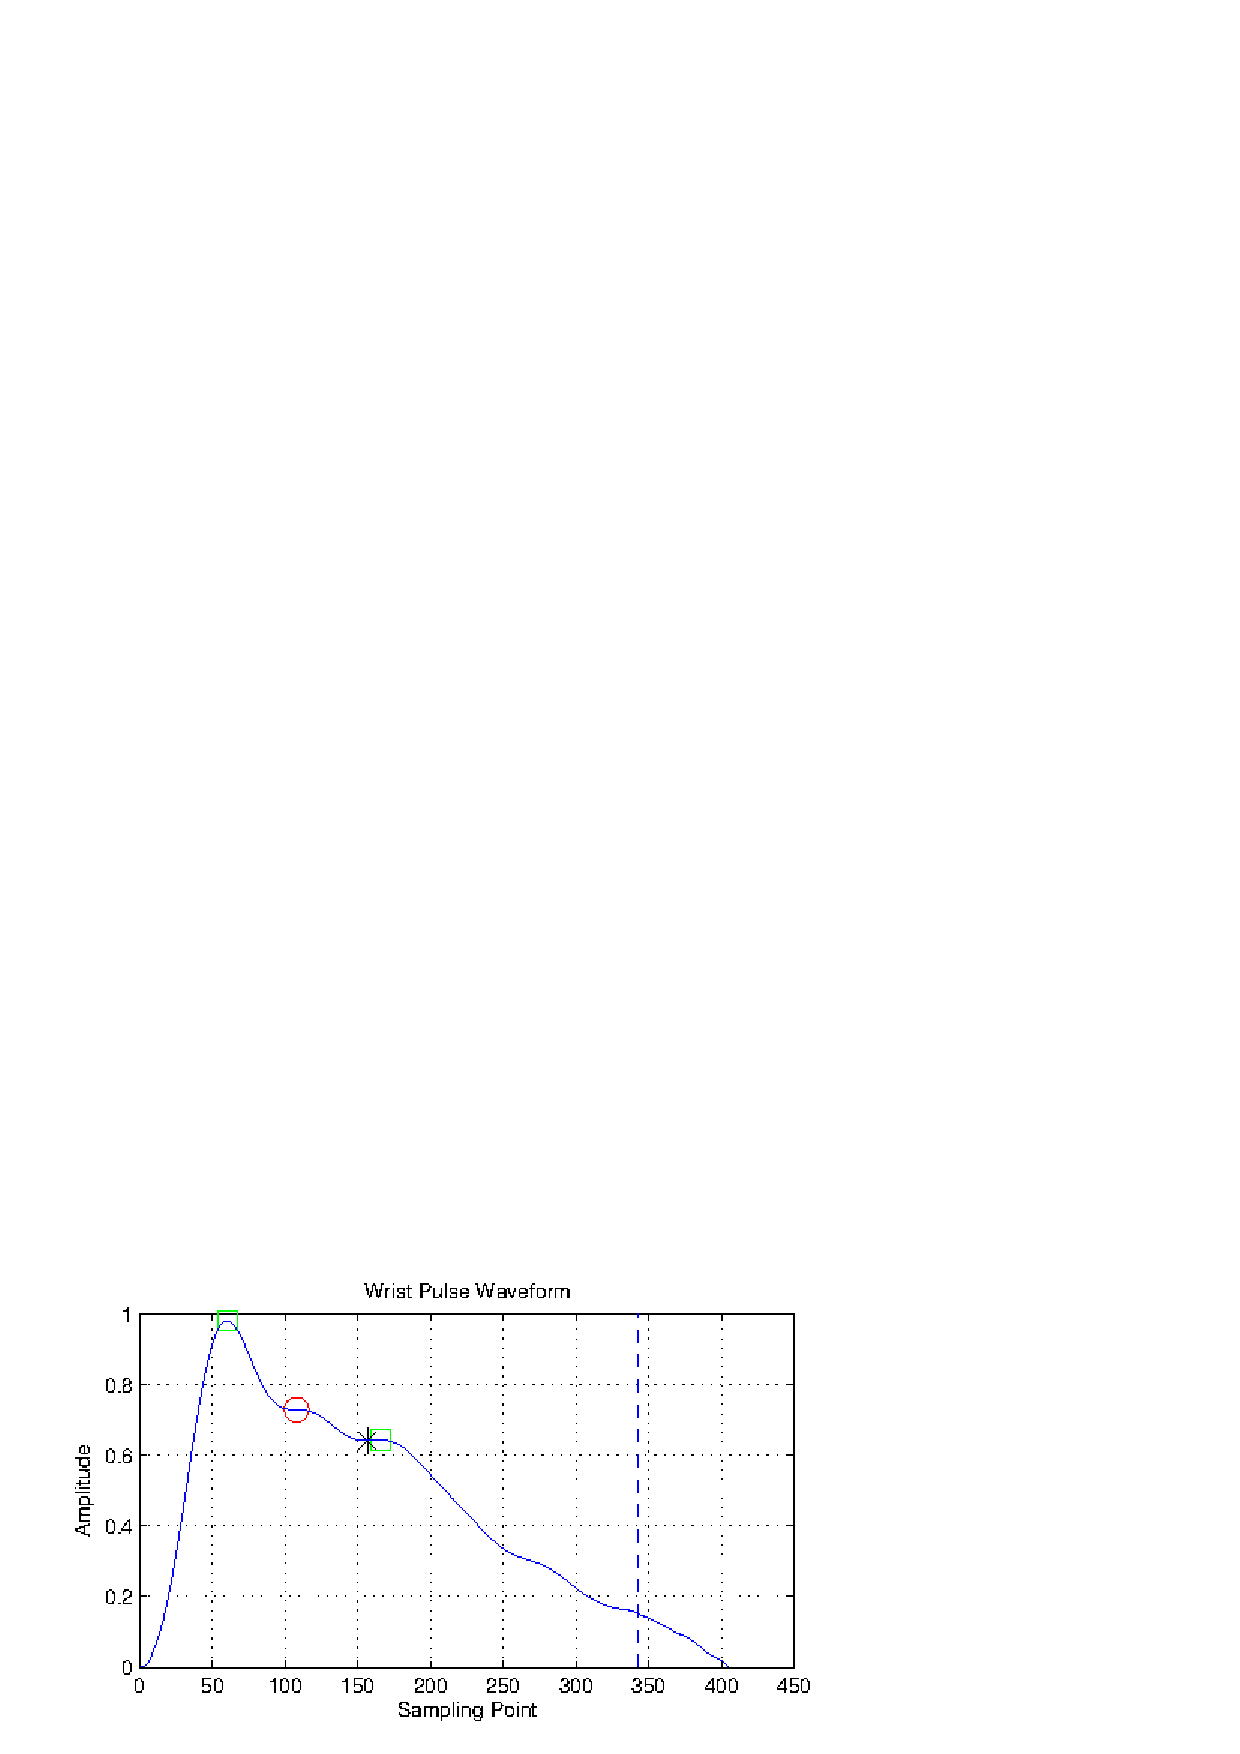
\includegraphics[width=0.7\textwidth]{hiddentidal}}\\
    \subfloat[The 1st-order
    difference]{\label{fig:1stdiff}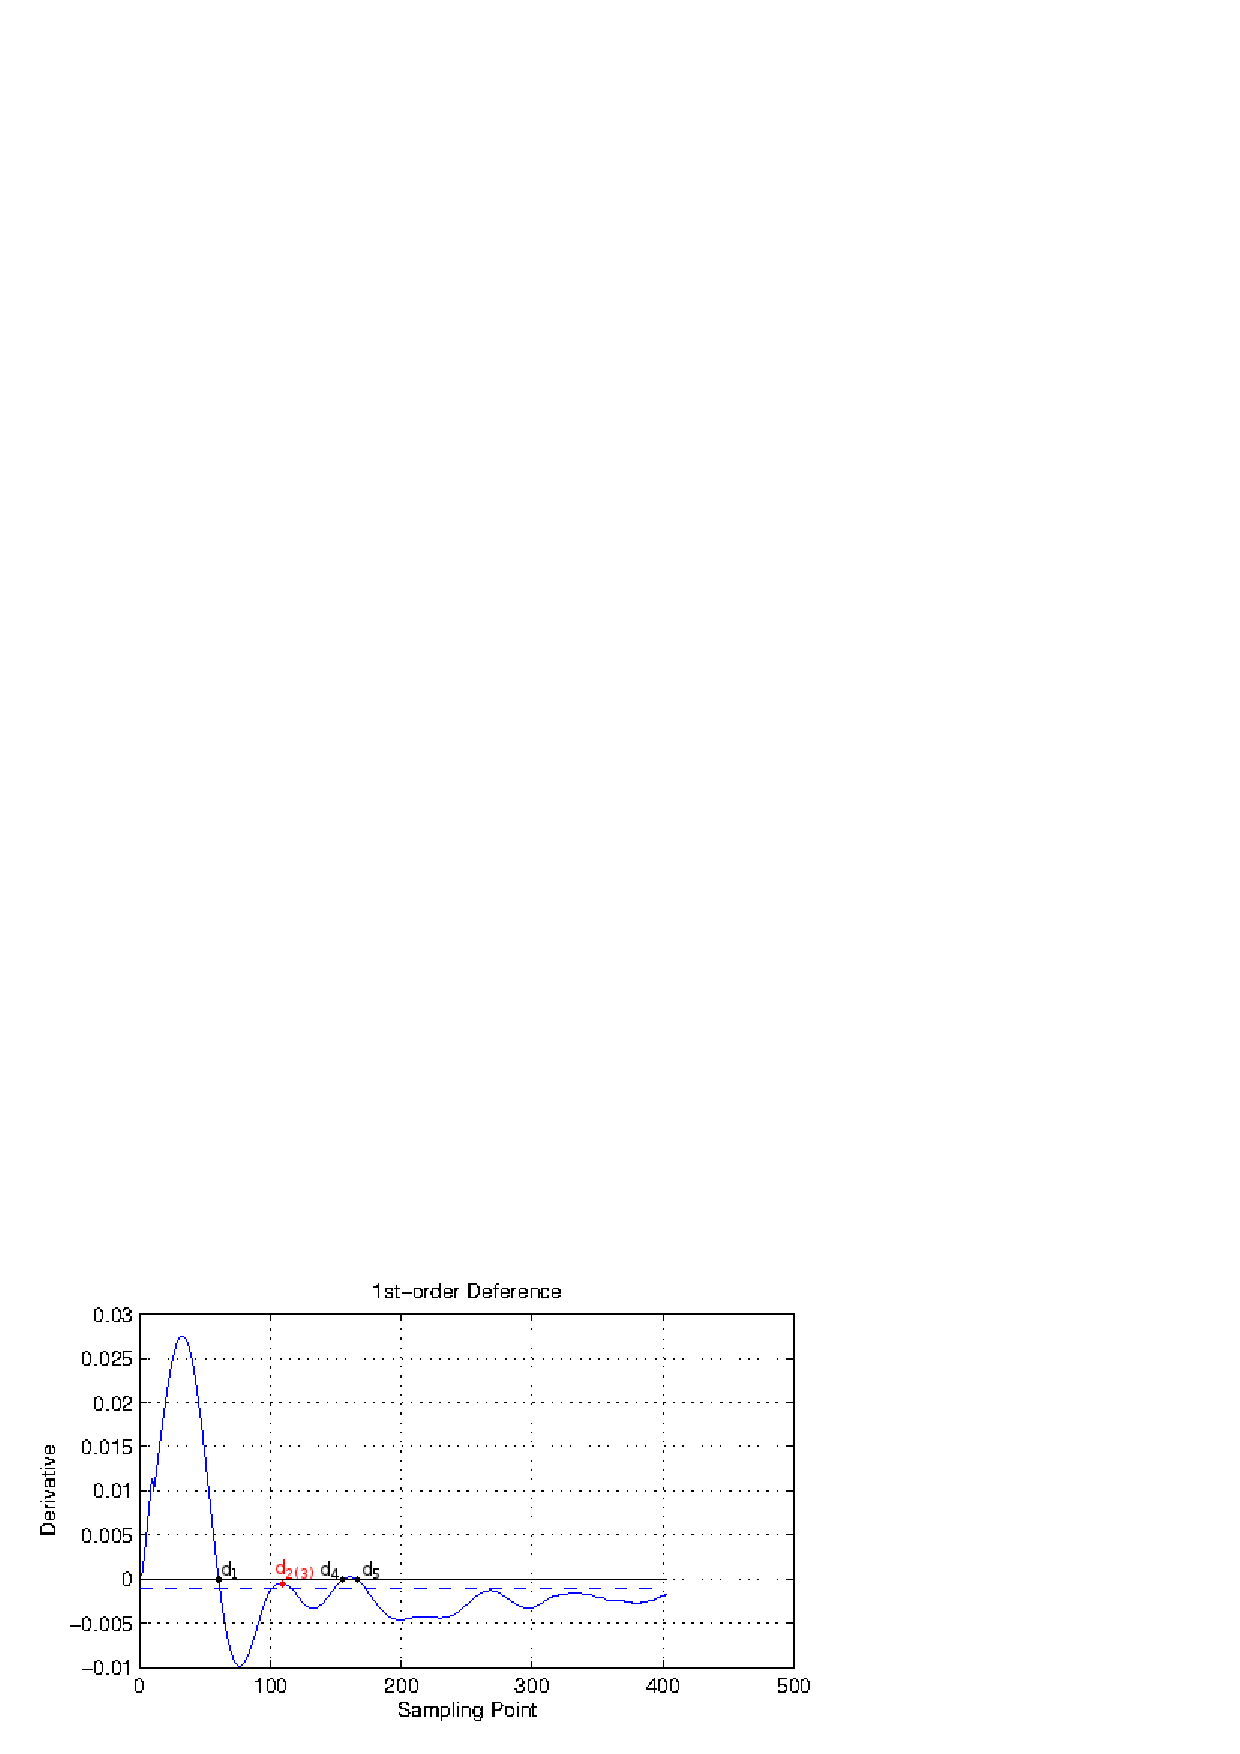
\includegraphics[width=0.7\textwidth]{1diff}}\\
    \subfloat[The 2nd-order
    difference]{\label{fig:2nddiff}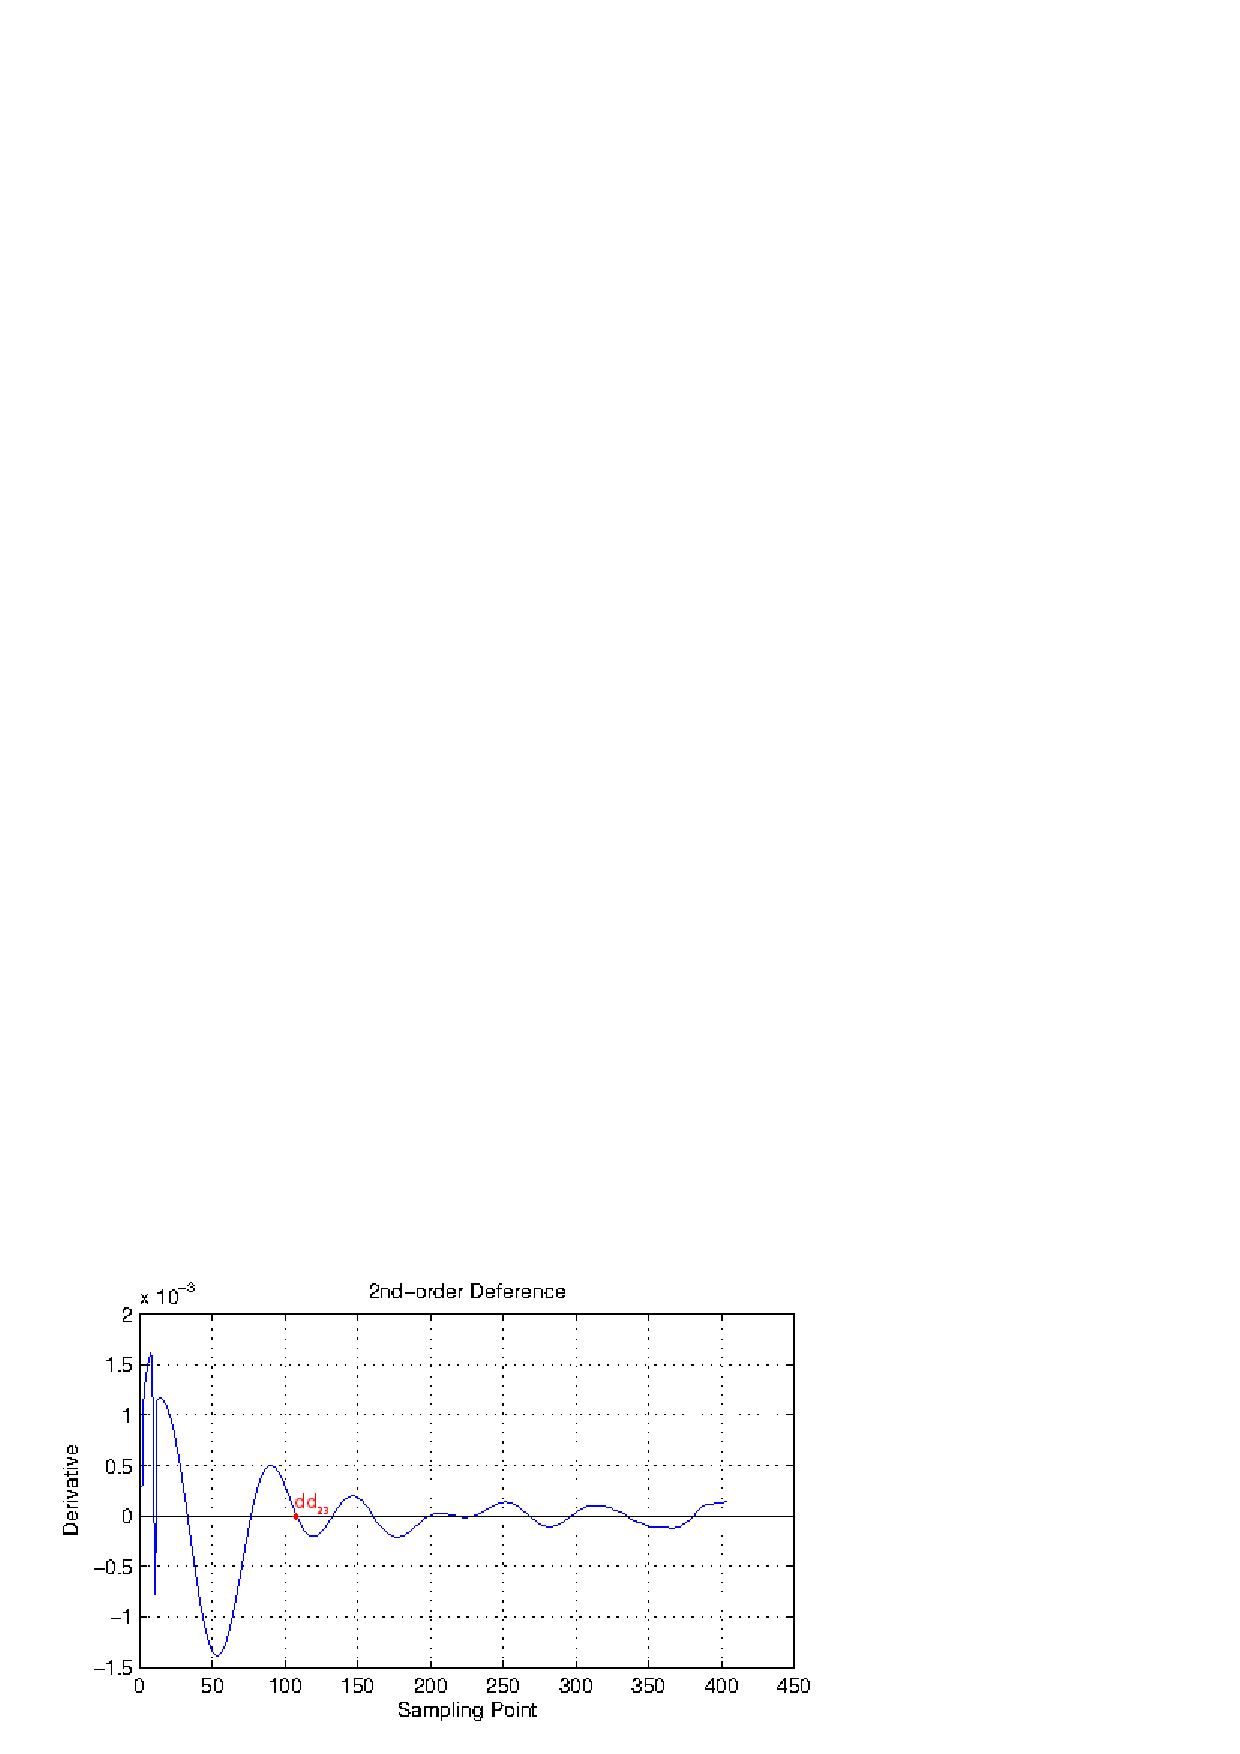
\includegraphics[width=0.7\textwidth]{2diff}}\\
    \caption{Illustration of the search of tidal wave}
    \label{fig:hiddentidal}
\end{figure}


\subsection{其他特征}

\todo{特征}

\chapter[Pulse pattern classification]{\uppercase{Pulse Pattern Classification}}
\label{chap:five}

The pulse pattern classification is the key to achieving automated
pulse diagnosis. The selection of classifier greatly influences the
accuracy of result. Each classifier has their own applicable
conditions, so the selection should depend on the characteristics of
sample sets, e.g. the size of data set, the distribution of
samples. Hitherto the common used classifiers includes Bayesian
classifier, linear classifier, artificial neural network (ANN), k-nearest
neighbor classifier (KNN), supporting vector machine (SVM) etc. \todo{选分类器}

\section{Support vector machine classifier}

\subsection{Principle of SVM}
Support vector machine is a supervised learning method to analyze
data and classify patterns. Based on statistical theory, the standard SVM 
is a non-probabilistic binary linear classifier since it takes a set
of input data and predicts, for each given input, which of two
possible classes comprises the input.
an SVM training algorithm builds a model
that assigns new examples into one category or the other. An SVM model
is a representation of the examples as points in space, mapped so that
the examples of the separate categories are divided by a clear gap
that is as wide as possible. New examples are then mapped into that
same space and decided the category based on the side they fall on.

\subsection{Experimental design}
\subsection{SVM classification result}

TODO

\section{Linear discriminant analysis classifier}

\subsection{Principle of LDA}
\subsection{Experimental design}
\subsection{LDA classification result}

TODO

\section{K-nearest neighbor classifier}

\subsection{Principle of KNN}
\subsection{Experimental design}
\subsection{KNN classification result}
TODO

\section{}<++>

\section{Summary}

TODO

% !Mode:: "TeX:UTF-8" 

\chapter[Conclusion]{\uppercase{Conclusion}}
   % 结论

%参考文献
\defaultfont
\bibliographystyle{unsrt}
\addcontentsline{toc}{chapter}{\bfseries  References} % 参考文献加入到英文目录
\addtolength{\bibsep}{-0.8em}
\nocite{*}  %若将此命令屏蔽掉,则未引用的文献不会出现在文后的参考文献中。
\bibliography{reference/reference}


%\include{appendix/appA}    % 附录
%\include{appendix/publications}    % 所发文章
%% !Mode:: "TeX:UTF-8" 

\newcommand{\subchapterstyle}%
  {\CJKfamily{hei}\rmfamily\bfseries\xiaoer}
\clearpage\BiAppendixChapter{哈\hspace{0.5pt}尔\hspace{0.5pt}滨\hspace{0.5pt}工\hspace{0.5pt}业\hspace{0.5pt}大\hspace{0.5pt}学\hspace{0.5pt}学\hspace{0.5pt}位\hspace{0.5pt}论\hspace{0.5pt}文\hspace{0.5pt}原\hspace{0.5pt}创\hspace{0.5pt}性\hspace{0.5pt}声\hspace{0.5pt}明\hspace{0.5pt}及\hspace{0.5pt}使\hspace{0.5pt}用\hspace{0.5pt}授\hspace{0.5pt}权\hspace{0.5pt}说\hspace{0.5pt}明}{\bfseries\xiaosi Statement of copyright and Letter of authorization}
\vspace{\baselineskip}
\begin{center}\hei\xiaosan{学位论文原创性声明}\end{center}
\vspace{1em}

本人郑重声明:此处所提交的学位论文《\chinesethesistitle》,是本人在导师指导下,在哈尔滨工业大学攻读学位期间独立进行研究工作所取得的成果。据本人所知,论文中除已注明部分外不包含他人已发表或撰写过的研究成果。对本文的研究工作做出重要贡献的个人和集体,均已在文中以明确方式注明。本声明的法律结果将完全由本人承担。

\vspace{\baselineskip}
\hspace{6em}作者签名:\hfill 日期:\hspace{2.5em}年\hspace{1.5em}月\hspace{1.5em}日

\vspace{3\baselineskip}
\begin{center}\hei\xiaosan{学位论文使用授权说明}\end{center}
\vspace{1em}

本人完全了解哈尔滨工业大学关于保存、使用学位论文的规定,即:

(1)已获学位的研究生必须按学校规定提交学位论文;(2)学校可以采用影印、缩印或其他复制手段保存研究生上交的学位论文;(3)为教学和科研目的,学校可以将学位论文作为资料在图书馆及校园网上提供目录检索与阅览服务;(4)根据相关要求,向国家图书馆报送学位论文。

保密论文在解密后遵守此规定。
\vspace{\baselineskip}

本人保证遵守上述规定。

\vspace{2\baselineskip}
\hspace{6em}作者签名:\hfill 日期:\hspace{2.5em}年\hspace{1.5em}月\hspace{1.5em}日

\vspace{2\baselineskip}
\hspace{6em}导师签名:\hfill 日期:\hspace{2.5em}年\hspace{1.5em}月\hspace{1.5em}日   % 承诺
%\include{appendix/acknowledgements}% 致谢

%\ifxueweidoctor
%\include{appendix/Resume}          % 博士学位论文有个人简介
%\fi
%\fi

\clearpage

\end{document} 
